\documentclass[11pt,letterpaper]{article}
\usepackage[margin=1.2in]{geometry}
\usepackage{amsmath, amssymb, amsthm}
\usepackage{bm}
\usepackage{hyperref}
\usepackage{enumitem}
\usepackage[dvipsnames]{xcolor}
\usepackage{setspace}
\usepackage{graphicx}
\usepackage{booktabs}
\usepackage{caption}
\usepackage{subcaption}
\usepackage{float}
\usepackage{microtype}
\usepackage{titlesec}
\usepackage[section]{placeins}
\usepackage{array}
\usepackage{tabularx}
\usepackage{longtable}
\usepackage{adjustbox}
\usepackage{colortbl}

%\usepackage{ALmacros}

\hypersetup{
	colorlinks=true,
	linkcolor=MidnightBlue,
	urlcolor=MidnightBlue,
	citecolor=MidnightBlue
}
\setstretch{1.0}
\raggedbottom

\makeatletter
\setlength{\@fptop}{0pt}
\setlength{\@fpsep}{8pt plus 2pt minus 2pt}
\setlength{\@fpbot}{0pt plus 1fil}
\makeatother
\renewcommand{\topfraction}{0.92}
\renewcommand{\bottomfraction}{0.85}
\renewcommand{\textfraction}{0.06}
\renewcommand{\floatpagefraction}{0.72}

\setlength{\parindent}{1.15em}
\setlength{\parskip}{0pt}
\setlength{\textfloatsep}{8pt plus 2pt minus 2pt}
\setlength{\floatsep}{7pt plus 2pt minus 2pt}
\setlength{\intextsep}{7pt plus 2pt minus 2pt}
\setlength{\abovecaptionskip}{4pt}
\setlength{\belowcaptionskip}{0pt}
\captionsetup{font=small,labelfont=bf,skip=4pt}
\titlespacing*{\section}{0pt}{1.3ex plus .4ex minus .2ex}{0.7ex plus .2ex}
\titlespacing*{\subsection}{0pt}{1.1ex plus .3ex minus .2ex}{0.5ex plus .1ex}
\titlespacing*{\subsubsection}{0pt}{0.9ex plus .2ex minus .1ex}{0.4ex plus .1ex}
\AtBeginDocument{\setlength{\abovedisplayskip}{6pt plus 2pt minus 2pt}\setlength{\belowdisplayskip}{6pt plus 2pt minus 2pt}\setlength{\abovedisplayshortskip}{4pt plus 2pt minus 2pt}\setlength{\belowdisplayshortskip}{4pt plus 2pt minus 2pt}}
\definecolor{virtblue}{HTML}{1f77b4}
\definecolor{illred}{HTML}{d62728}
\definecolor{accentgreen}{HTML}{2ca02c}
\definecolor{lightgray}{gray}{0.92}
\definecolor{boxblue}{HTML}{E8F0FE}

\graphicspath{{../figures/}{../notebooks/plots/}{.}}

\newcommand{\psimax}{\psi_{\max}}
\newcommand{\psibar}{\bar{\psi}}
\newcommand{\rhopsi}{\rho_{\psi}}
\newcommand{\gr}{\mathrm{Gr}}
\newcommand{\tr}{\mathrm{tr}}
\newcommand{\dproj}{d_{\mathrm{proj}}}
\newcommand{\erank}{\mathrm{erank}}

\newcommand{\bR}{\mathbb{R}}
\newcommand{\cA}{\mathcal{A}}
\newcommand{\cB}{\mathcal{B}}
\newcommand{\cJ}{\mathcal{J}}
\newcommand{\cL}{\mathcal{L}}
\newcommand{\cS}{\mathcal{S}}
\newcommand{\eE}{\mathsf{E}}
\newcommand{\eH}{\mathsf{H}}

\newtheorem{theorem}{Theorem}[section]
%\newtheorem{algorithm}[theorem]{Algorithm}
\newtheorem{corollary}[theorem]{Corollary}
\newtheorem{criterion}[theorem]{Criterion}
\newtheorem{definition}[theorem]{Definition}
\newtheorem{lemma}[theorem]{Lemma}
\newtheorem{proposition}[theorem]{Proposition}

\pagestyle{myheadings} \markboth{A. Deep, A. Lesniewski, O. Missaoui, and C. Pakala}{Geometry of the Virtue of Complexity}

\begin{document}
	
\title{From Parameters to Subspaces: The Geometry of Complexity in Asset Pricing}
\author{Arsh Deep, Andrew Lesniewski, Oualid Missaoui, and Chaithanya Pakala\thanks{This paper reflects the views of the authors only and does not necessarily represent the views of their employers or affiliated institutions.}\\
Department of Mathematics\\
Baruch College\\
One Bernard Baruch Way\\
New York, NY 10010\\
USA}
\date{\today}
\maketitle


\begin{abstract}
Recent debates in empirical asset pricing ask whether the performance gains of high-dimensional machine-learning models reflect genuine economic structure or statistical illusion. We argue that this question is fundamentally geometric. Across a broad class of conditional factor models, nonlinear exposure maps and
high-dimensional feature expansions ultimately generate low-dimensional return-producing subspaces. The economically relevant object is therefore not the raw parameter vector, but a point, or trajectory, on a Grassmann manifold. This perspective separates parameter complexity from structural complexity: additional parameters are useful only when they expand a stable and identifiable return signal subspace. We develop Grassmannian diagnostics for subspace stability, intrinsic dimension, curvature, effective rank, and spectral separation, and use them to distinguish adaptive complexity from diffuse overparameterization. In synthetic experiments and historical RFF--IPCA backtests, these diagnostics identify frozen configurations, locate empirical signal boundaries, and explain why the best-performing models lie in a Goldilocks region of stable but nontrivial subspace motion. The results provide a geometric framework for evaluating the virtue of complexity in asset pricing.
\end{abstract}
\bigskip\noindent
\textbf{Keywords:} Asset pricing, conditional factor models, Grassmann manifold, intrinsic dimension, model complexity, machine learning.
\newpage

\section{Introduction}
\label{sec:intro}

Recent work in empirical asset pricing argues that nonlinear and high-dimensional machine-learning models can substantially improve the estimation of stochastic discount factors, conditional factor structures, and return forecasts \cite{GKX20, KMZ24}. At the same time, these findings raise a central question: do the gains from complexity reflect genuine economic structure, or are they artifacts of overfitting, regularization, and high-dimensional statistical noise?

Recent work has also clarified that complexity and parsimony need not be opposing principles. For example, \cite{AL26} distinguish capacity sparsity from factor sparsity and show that large nonlinear feature expansions can improve out-of-sample SDF performance when combined with sparse selection. Their findings suggest that complexity may be valuable because it enlarges the search space from which a parsimonious pricing structure can be identified. The present paper is complementary in spirit but different in emphasis. Rather than studying sparsity in a particular coordinate representation, we study the geometry of the return-producing subspaces induced by complex predictive models.

Our starting point is simple. Many conditional factor models, regardless of how their exposures are parameterized, ultimately produce a low-rank representation of returns. This is explicit in Instrumented Principal Component Analysis (IPCA) and related characteristic-based factor models \cite{KPS19}, and it remains true after nonlinear feature expansion. Let $N$ denote the number of assets and $k$ the number of latent factors. At each time $t$, cross-sectional returns $r_t\in\bR^N$ are approximated by
\begin{equation}
r_t \approx \beta_t^\top f_t,
\end{equation}
where $\beta_t\in\mathrm{Mat}_{k,N}(\bR)$ and $f_t\in\bR^k$. The rule that generates the exposure matrix $\beta_t$ from the information available at date $t$ will be called the \emph{exposure map}. At a formal level, we may write
\begin{equation}
\cB_\theta : t \mapsto \beta_t(\theta),
\end{equation}
where $\theta$ denotes the parameters of the model. In a characteristic-based linear model, $\cB_\theta$ is induced by a linear loading map. In lifted or nonlinear models, it may depend on nonlinear transformations of characteristics or other flexible architectural choices.

For a fixed date $t$, the fitted return component $\beta_t(\theta)^\top f_t$ does not range over all of $\bR^N$. It lies in the linear span of the columns of $\beta_t(\theta)^\top$. We therefore define the associated return-producing subspace by
\begin{equation*}
V_t(\theta) = \operatorname{span}\bigl(\beta_t(\theta)^\top\bigr) \in \gr(k,N),
\end{equation*}
where $\gr(k,N)$ denotes the Grassmann manifold of $k$-dimensional subspaces of $\bR^N$ \cite{AMS08, B23, BZA24}. As time evolves, the fitted model induces a trajectory
$t \mapsto V_t(\theta)$ on $\gr(k,N)$.

This subspace representation removes a basic non-identification in factor models. For any orthogonal matrix $O\in O(k)$, replacing $\beta_t$ by $O\beta_t$ and $f_t$ by $Of_t$ leaves the fitted return component unchanged:
\begin{equation*}
	(O\beta_t)^\top(Of_t)=\beta_t^\top f_t.
\end{equation*}
Thus, the particular coordinates used to represent the latent factor space are not economically meaningful. More generally, distinct parameterizations of the exposure map may induce the same trajectory of return-producing subspaces. From an economic perspective, the relevant object is therefore not the particular parameter vector $\theta$, nor even the specific matrix representation $\beta_t(\theta)$, but the induced path $t \mapsto V_t(\theta)$ on $\gr(k,N)$. In the projection-based factor models studied below, this is precisely the object seen by the concentrated least-squares criterion: the loss depends on the orthogonal projector onto $V_t(\theta)$, not on the arbitrary basis used to represent that subspace.

This observation leads to a geometric reframing of the virtue-of-complexity debate. It separates two notions of complexity. \emph{Parameter complexity} refers to the dimension, nonlinearity, or flexibility of the estimation architecture: additional characteristics, richer feature lifts, larger dictionaries, or more expressive models. \emph{Structural complexity} refers to the effective dimension, stability, curvature, and persistence of the induced return-producing subspace trajectory. From this perspective, increasing model complexity can have three distinct effects. It can be \emph{meaningful}, if it enlarges the family of admissible return-subspace trajectories in a stable and identifiable way. It can be \emph{redundant}, if it merely re-expresses essentially the same subspaces in different coordinates. Or it can be \emph{illusory}, if it introduces weakly identified directions that appear flexible in sample but rotate under sampling variation without adding persistent return structure.

The central question of the paper is therefore:
\begin{quote}
	Does increasing functional complexity enlarge the induced trajectory on $\gr(k,N)$ in a stable, identifiable, and economically persistent manner?
\end{quote}

In this formulation, functional complexity enlarges the class of admissible exposure maps $\cB_\theta : t \mapsto \beta_t(\theta)$, and hence the class of admissible Grassmannian trajectories at fixed rank $k$:
\begin{equation*}
t \mapsto V_t(\theta)\in\gr(k,N).
\end{equation*}
The nominal factor dimension $k$ fixes the dimension of each fitted subspace, but it does not by itself determine how much stable return structure has been learned. A model with many parameters may still produce a nearly frozen or effectively low-dimensional path, while a more flexible model may generate additional persistent directions of return variation. Complexity is virtuous when it expands the stable signal-bearing component of the return span. It is illusory when the added degrees of freedom appear mainly as unstable rotations in weak or nearly flat directions.

Our contribution is to formalize this distinction and to turn it into an empirical diagnostic framework. We first show that, for projection-based conditional factor models, the economically relevant fitted object is the induced return subspace rather than a unique parameterization of the exposure map. After profiling out the latent factors, the objective depends on the orthogonal projector onto
\begin{equation*}
V_t(\theta)=\operatorname{span}\bigl(\beta_t(\theta)^\top\bigr),
\end{equation*}
not on the particular coordinates used to represent that subspace. This provides the formal link between conditional factor estimation and Grassmannian geometry.

We then study the local geometry of the associated projection functional. In a stylized population setting, the signal component of returns spans an effective subspace of dimension $k_0$. When the nominal fitted dimension $k$ exceeds this effective signal dimension, the additional directions are not identified by population fit. Geometrically, the objective becomes flat, or nearly flat, along rotations that move these extra directions inside the noise eigenspace. Thus overparameterization does not necessarily create new return structure; it may instead create directions that are available to the estimator but weakly pinned down by the data.

This curvature picture yields concrete empirical implications. Weakly identified directions should appear as spectral-gap collapse, loss of effective rank, and unstable or diffuse subspace motion across rolling windows. Conversely, useful complexity should appear as stable expansion of the signal-bearing return span. The paper therefore develops a set of Grassmannian diagnostics to distinguish these cases. Projection distance measures whether a fitted subspace is frozen near its warm start or moving meaningfully through the Grassmannian. Principal-angle diagnostics decompose that motion across directions: for two fitted
subspaces with orthonormal bases $U_1$ and $U_2$, the principal angles
$\psi_1,\ldots,\psi_k$ are defined by
$\cos\psi_j=\sigma_j(U_1^\top U_2)$ and measure directional rotations between
the subspaces. The anisotropy ratio
\begin{equation*}
\rho_\psi=\frac{\bar\psi}{\psi_{\max}}
\end{equation*}
measures whether subspace motion is concentrated in a small number of directions or spread diffusely across many directions. Effective rank and spectral gap locate empirical signal boundaries. Together, these quantities distinguish \emph{regime separators}, which identify whether a configuration lies in a frozen, active, or weakly identified regime, from \emph{within-regime diagnostics}, which help rank configurations once the model is genuinely active.

We apply the framework in two settings. First, synthetic experiments provide a controlled environment in which the true signal dimension is known. These experiments validate that the Grassmannian diagnostics recover the expected regime structure and identify when overparameterization creates weakly identified directions. Second, we study an empirical asset-pricing application based on Random Fourier Feature (RFF) lifted IPCA models. This application asks whether the same geometric mechanisms are visible in a visible in an empirical return-prediction environment, where the true signal dimension is unknown and the fitted subspaces must be inferred from characteristics and realized returns. The results reveal a spectral-gap cliff, a Goldilocks region of subspace movement, and a strong association between concentrated subspace drift and higher out-of-sample Sharpe ratios. The extended empirical analysis further shows how factor count, RFF dimension, and training-window length interact through the same geometric mechanisms.

The present paper focuses on linear IPCA and lifted linear extensions based on Random Fourier Features \cite{RR07, RR08}. This choice is deliberate. RFF lifts provide a clean intermediate case: they enlarge the nonlinear characteristic dictionary while preserving a linear Grassmannian estimator conditional on the lifted features. They therefore allow us to study the geometry of functional complexity without conflating it with the additional optimization and architectural issues of fully nonlinear models.

Fully nonlinear exposure maps, including neural-network specifications, fit naturally into the same geometric framework. They also generate return-producing subspaces, but the map from characteristics to subspaces is itself learned through a nonlinear architecture. We defer those models to a companion paper, where the role of architecture, regularization, and nonlinear subspace stability will be studied in detail.

The remainder of the paper is organized as follows. Section~\ref{sec:ipca} uses IPCA as a prototype to show how conditional factor models induce Grassmannian return subspaces. Section~\ref{sec:rff} introduces Random Fourier Feature lifts as a controlled way to enlarge the nonlinear characteristic dictionary while preserving a linear Grassmannian estimation problem. Section~\ref{sec:ret_subspaces} develops the geometric diagnostics used throughout the paper, including projection distance, principal angles, effective rank, and spectral-gap measures. Section~\ref{sec:pop_setup} introduces the population signal-plus-noise setup used to distinguish identified signal directions from weak or flat noise directions. Section~\ref{sec:curvature} analyzes the curvature and identification structure of the population objective. Section~\ref{sec:geom_tests} connects these diagnostics to the distinction between parameter complexity and structural complexity. Section~\ref{sec:simulated} presents synthetic experiments that validate the diagnostics in a controlled setting. Section~\ref{sec:hist_data} applies the framework to the asset pricing   experiment and studies the spectral-gap cliff, anisotropy, Goldilocks stability region, and extended robustness backtests. Section~\ref{sec:pract_use} summarizes practitioner uses of the diagnostics for model screening, regularization choice, factor-dimension selection, feature expansion, and runtime monitoring. Section~\ref{sec:conclusion} concludes. Appendices~\ref{sec:grass_geom} and~\ref{sec:proofs} contain a summary of background facts on Grassmannian geometry and the proofs of the population theorems, respectively.


\section{IPCA as a Prototype: From Parameters to Subspaces}
\label{sec:ipca}

%We use the linear IPCA model of \cite{KPS19, KPS20} as a transparent prototype for the geometric structure underlying conditional factor models. The point of the %reformulation is simple: although IPCA is usually written in terms of a parameter matrix, the identified object is a subspace. This makes IPCA a natural entry point into %the Grassmannian viewpoint developed in this paper. We follow the geometric interpretation in \cite{LM26}.

We use the linear IPCA model of \cite{KPS19,KPS20} as a transparent prototype for the geometric structure underlying conditional factor models. In its standard formulation, IPCA is written as an optimization over a loading matrix and latent factors, which can make the parameter matrix appear to be the primary object of interest. The geometric reformulation emphasizes that this is not quite right: because the latent factor representation is invariant to rotations of the factor basis, the matrix representation is not uniquely identified. What is identified is the subspace selected by the loading matrix, together with the sequence of return-producing subspaces induced by the observed characteristics over time. Thus IPCA already contains, in a simple linear setting, the central geometric feature of more general conditional factor models: fitted returns depend on projections onto low-dimensional subspaces rather than on a particular coordinate representation of those subspaces. This makes IPCA a natural entry point into the Grassmannian viewpoint developed in this paper. We follow the geometric interpretation in \cite{LM26}.

\subsection{The IPCA specification}
\label{sec:ipca:spec}

At each date $t$, let $r_t\in \bR^N$ denote the vector of cross-sectional returns and let $Z_t\in\mathrm{Mat}_{N,m}(\bR)$ denote the matrix of asset characteristics. In linear IPCA, asset exposures are generated from characteristics through a loading map
\begin{equation*}
\beta_t = \Gamma Z_t^\top, \qquad \Gamma\in \mathrm{Mat}_{k,m}(\bR),
\end{equation*}
where $k$ is the number of latent factors. In the terminology of the Introduction, linear IPCA defines the exposure map
\begin{equation*}
\cB_\Gamma : t \mapsto \beta_t(\Gamma)=\Gamma Z_t^\top .
\end{equation*}
The parameter matrix $\Gamma$ and the characteristic matrix $Z_t$ therefore jointly determine the date-$t$ exposure matrix. Equivalently, returns are modeled as
\begin{equation*}
r_t=Z_t\Gamma^\top f_t+\varepsilon_t,\qquad f_t\in \bR^k.
\end{equation*}
Here $\Gamma$ maps the $m$-dimensional characteristic space into a $k$-dimensional factor-exposure space. The standard IPCA estimator solves
\begin{equation*}
\min_{\Gamma,\{f_t\}}\,\frac{1}{T}\,\sum_{t=1}^T \|r_t-Z_t\Gamma^\top f_t\|^2.
\end{equation*}

\subsection{Rotational invariance and the Grassmann parameter}
\label{sec:ipca:grassmann}

The factor representation is not unique. For any orthogonal matrix $O\in O(k)$, the transformation
\begin{equation*}
\Gamma \mapsto O\Gamma, \qquad f_t \mapsto Of_t
\end{equation*}
leaves the fitted return component unchanged:
\begin{equation*}
Z_t (O\Gamma)^\top (Of_t)=Z_t\Gamma^\top f_t.
\end{equation*}
Therefore $\Gamma$ is not identified as a matrix; only its row space is identified:
\begin{equation*}
\operatorname{row}(\Gamma) = \operatorname{span}(\Gamma^\top)
\in \gr(k,m).
\end{equation*}

This is the first Grassmannian structure in IPCA. The economically relevant parameter is not a particular basis for the factor space, but the $k$-dimensional characteristic subspace selected by the rows of $\Gamma$.

\subsection{Profiling out factors: a projection objective}
\label{sec:ipca:projection}

For a fixed $\Gamma$, define the date $t$ loading matrix
\begin{equation*}
\Lambda_t(\Gamma)=Z_t\Gamma^\top\in \mathrm{Mat}_{N,k}(\bR).
\end{equation*}
The least-squares factor estimate is
\begin{equation*}
f_t^*(\Gamma)=\bigl(\Lambda_t^\top\Lambda_t\bigr)^{-1}\Lambda_t^\top r_t,
\end{equation*}
assuming $\Lambda_t^\top\Lambda_t$ is nonsingular. Substituting this expression back into the objective gives the concentrated loss
\begin{equation*}
\cL(\Gamma)=\frac{1}{T}\,\sum_{t=1}^T \|(I-P_t(\Gamma))r_t\|^2,
\end{equation*}
where
\begin{equation*}
P_t(\Gamma)=\Lambda_t\bigl(\Lambda_t^\top\Lambda_t\bigr)^{-1}\Lambda_t^\top
\end{equation*}
is the orthogonal projector onto the fitted return span
\begin{equation*}
V_t(\Gamma) = \operatorname{span}\bigl(Z_t\Gamma^\top\bigr)
\in \gr(k,N).
\end{equation*}

The concentrated IPCA objective therefore depends on $\Gamma$ only through the sequence of return subspaces
\begin{equation*}
t\longmapsto V_t(\Gamma)\in \gr(k,N).
\end{equation*}
Equivalently, IPCA minimizes the projection error
\begin{equation*}
\cJ(V)=\frac{1}{T}\,\sum_{t=1}^T\|(I-\Pi_{V_t})r_t\|^2
\end{equation*}
over the admissible family
\begin{equation*}
\cA=\big\{(V_t)_{t=1}^T:V_t=\operatorname{span}(Z_t\Gamma^\top),\text{ for some } \Gamma\in\mathrm{Mat}_{k,m}(\bR)\big\}.
\end{equation*}

This reformulation is the key geometric point. IPCA is usually presented as an optimization over the matrix $\Gamma$, but the loss only sees the $k$-dimensional subspaces generated by $Z_t\Gamma^\top$. Parameter complexity therefore affects the family of attainable return subspaces, while the objective itself measures the projection of returns onto those subspaces. In this sense, IPCA already operates on Grassmannian objects: a characteristic subspace $\operatorname{row}(\Gamma)\in\gr(k,m)$ induces a time series of return subspaces $V_t(\Gamma)\in\gr(k,N)$.

The same viewpoint extends directly to nonlinear feature maps and macro-conditioned specifications. Replacing $Z_t$ by an expanded feature
matrix changes the ambient characteristic space in which $\operatorname{row}(\Gamma)$ lives, but the fitted object remains a $k$-dimensional return subspace. Likewise, macro conditioning \cite{LM26} changes the way the factor span evolves across states, but not the underlying Grassmannian interpretation: the model is still selecting, rotating, and regularizing low-dimensional subspaces.

\section{Lifted Linear Models and Random Fourier Features}
\label{sec:rff}

The linear IPCA specification in Section~\ref{sec:ipca} uses characteristics directly to generate conditional exposures. A natural extension is to replace the raw characteristics by a higher-dimensional nonlinear feature representation while retaining a linear factor structure. This produces a class of \emph{lifted linear models}: models that are nonlinear in the original characteristics but linear in the lifted feature space.

Let
\begin{equation}
\label{eq:liftedlinspec}
\beta_t=\Gamma \Phi(Z_t)^\top,\qquad\Gamma \in \mathrm{Mat}_{k,\tilde m}(\bR),
\end{equation}
where $Z_t\in \mathrm{Mat}_{N,m}(\bR)$ collects asset characteristics and
\begin{equation*}
\Phi(Z_t)\in \mathrm{Mat}_{N,\tilde m}(\bR)
\end{equation*}
is a lifted feature matrix. In the exposure-map notation of the Introduction, the lifted model corresponds to
\begin{equation*}
\cB_\Gamma^\Phi : t \mapsto \beta_t(\Gamma)=\Gamma\Phi(Z_t)^\top .
\end{equation*}
Thus feature lifting changes the map from characteristics to exposures by replacing the raw characteristic matrix $Z_t$ with the lifted feature matrix $\Phi(Z_t)$. When $\tilde m \gg m$, the model has substantially greater parameter flexibility than linear IPCA. However, for each date $t$, fitted returns still lie in the rank-$k$ subspace
\begin{equation}
\label{eq:rff-subspace}
V_t(\Gamma)=\mathrm{span}\big(\Phi(Z_t)\Gamma^\top\big) \in \gr(k,N).
\end{equation}
Thus feature lifting enlarges the admissible family of exposure maps, and hence the family of attainable return subspaces, but it does not change the intrinsic rank of the return representation.

\subsection{Random Fourier Feature lifting}
\label{subsec:rff-lifting}

A canonical example of feature lifting is provided by \emph{Random Fourier Features} (RFF) \cite{RR07,RR08}. For a characteristic vector $z_{i,t}\in\bR^m$, define
\begin{equation}
\label{eq:rff-map}
\phi(z_{i,t})=\sqrt{\frac{2}{\tilde m}}\,
\big(
\cos(\omega_1^\top z_{i,t}+b_1),\dots,
\cos(\omega_{\tilde m}^\top z_{i,t}+b_{\tilde m})
\big)^\top,
\end{equation}
where $\omega_j\sim p(\omega)$ and $b_j\sim\mathrm{Unif}[0,2\pi]$. Stacking the transformed characteristics across assets gives
\begin{equation}
\label{eq:rff-design}
\Phi(Z_t)=
\begin{pmatrix}
\phi(z_{1,t})^\top \\
\vdots             \\
\phi(z_{N,t})^\top
\end{pmatrix}.
\end{equation}
The resulting Random Fourier Feature conditional factor model is
\begin{equation}
\label{eq:rff-factor-model}
r_t \approx \Phi(Z_t)\Gamma^\top f_t,
\end{equation}
where $f_t\in\bR^k$ are latent factors. This specification preserves the IPCA structure after replacing the original characteristic matrix $Z_t$ by the \emph{lifted matrix} $\Phi(Z_t)$.

Thus RFF lifting is a concrete realization of the lifted exposure map
\begin{equation*}
\cB_\Gamma^\Phi : t \mapsto \Gamma\Phi(Z_t)^\top,
\end{equation*}
with $\Phi$ generated by randomized nonlinear features. The resulting model is nonlinear in the original characteristics but remains linear in the lifted feature space.

\subsection{Profiled objective function}
\label{subsec:rff-profiled-objective}

As in IPCA, the factors can be profiled out explicitly. Define
\begin{equation}
\label{eq:rff-lambda}
\Lambda_t(\Gamma)=\Phi(Z_t)\Gamma^\top \in \mathrm{Mat}_{N,k}(\bR).
\end{equation}
For fixed $\Gamma$, the least-squares factor estimate is
\begin{equation}
\label{eq:rff-factor-profile}
f_t^*(\Gamma) = \big(\Lambda_t^\top\Lambda_t\big)^{-1} \Lambda_t^\top r_t,
\end{equation}
assuming $\Lambda_t^\top\Lambda_t$ is nonsingular. Substituting this expression into the least-squares objective yields the concentrated loss
\begin{equation}
\label{eq:rff-profiled}
\cL(\Gamma)=\frac{1}{T}\,\sum_{t=1}^T \|(I-P_t(\Gamma))r_t\|^2,
\end{equation}
where
\begin{equation}
\label{eq:rff-projector}
P_t(\Gamma)=\Lambda_t(\Gamma)\big(\Lambda_t^\top\Lambda_t\big)^{-1}\Lambda_t(\Gamma)^\top
\end{equation}
is the orthogonal projector onto
\begin{equation}
\label{eq:rff-return-subspace}
V_t(\Gamma) = \mathrm{span}\big(\Lambda_t(\Gamma)\big).
\end{equation}
Thus the lifted model leads to the same geometric form as IPCA: estimation minimizes a projection error onto a time-varying family of $k$-dimensional return subspaces.

\subsection{Geometry of lifted linear complexity}
\label{subsec:rff-geometry}

The key distinction between linear IPCA and the lifted model is not the dimension of the fitted return space at a given date. In both cases, fitted returns lie in a $k$-dimensional subspace of $\bR^N$. The distinction is instead the size and flexibility of the admissible family
\begin{equation}
\label{eq:rff-grassmann-trajectory}
t\mapsto V_t(\Gamma)\in\gr(k,N).
\end{equation}
Replacing $Z_t$ by $\Phi(Z_t)$ allows the model to generate richer Grassmann trajectories, because the exposures are linear combinations of nonlinear transformations of the original characteristics.

This observation separates parameter complexity from structural complexity.


Put differently, the lifted model does not gain structural complexity by increasing the rank of the fitted return representation at a fixed date; that rank remains $k$. It gains complexity by enlarging the set of subspace paths that the model can trace as characteristics evolve over time. This distinction matters because a larger feature dictionary may either reveal stable directions of return variation that were inaccessible to linear IPCA, or merely provide many redundant coordinates for describing essentially the same fitted subspaces.

 Increasing $\tilde m$ increases the number of parameters in $\Gamma$ and enlarges the feature span available to the model. However, the economically relevant object remains the induced return subspace $V_t(\Gamma)$, not the particular basis used to represent it. Indeed, for any $O\in O(k)$, the transformation
\begin{equation}
\Gamma \mapsto O\Gamma,\qquad f_t \mapsto Of_t,
\end{equation}
leaves fitted returns unchanged. The model is therefore identified only through the row space of $\Gamma$ and, date by date, through the induced subspace $V_t(\Gamma)$.

%Consequently, the virtue of feature complexity should not be evaluated by raw parameter counts alone. Additional features are useful only when they enlarge the %identified return subspace in a stable manner. In empirical applications, this motivates diagnostics based on Grassmannian quantities such as effective rank, principal %angles, and rolling-window stability of the fitted subspaces. If additional lifted features merely introduce weakly identified directions, the result may be subspace %instability rather than genuine improvement in predictive structure.

Consequently, the virtue of feature complexity should not be evaluated by raw parameter counts alone. Additional features are useful only when they enlarge the identified return subspace in a stable manner. Here stability does not mean that the fitted return subspace is fixed over time. Rather, it means that the additional directions uncovered by the feature expansion are sufficiently identified to persist across neighboring rolling windows, resamples, or random feature draws, and that any movement of the subspace trajectory is structured rather than diffuse. Regime changes are therefore not ruled out: they should appear as coherent shifts in the trajectory $t \mapsto V_t(\Gamma)$, ideally concentrated in a small number of principal directions, rather than as arbitrary rotations of weakly identified directions. In empirical applications, this motivates diagnostics based on Grassmannian quantities such as effective rank, principal angles, and rolling-window stability of the fitted subspaces. If additional lifted features merely introduce weakly identified directions, the result may be subspace instability rather than genuine improvement in predictive structure.

\section{Return Subspace Diagnostics on the Grassmann Manifold}
\label{sec:ret_subspaces}

%The preceding sections show that IPCA and its lifted linear extensions generate fitted returns through time-varying $k$-dimensional subspaces $V_t \in \gr(k,N)$. This %section introduces the diagnostics used to evaluate whether additional model flexibility produces genuine geometric structure or merely weakly identified directions. %The two central quantities are intrinsic dimensionality, measured through effective rank, and subspace stability, measured through principal angles and Grassmannian %distances.

The preceding sections recast IPCA and its lifted linear extensions as procedures that do not merely estimate parameter matrices, but induce trajectories of return-producing subspaces, $t \mapsto V_t \in Gr(k,N)$. Once the fitted object is viewed in this way, model assessment becomes a geometric problem. A more flexible model is useful only if it changes the induced subspace trajectory in a way that is both substantively richer and statistically identifiable. This section introduces diagnostics for making that distinction. The first set of diagnostics measures intrinsic dimensionality: how many fitted directions are effectively active in the return representation. The second set measures subspace stability: not whether the subspace is fixed over time, but whether its movement across rolling windows, resamples, or model perturbations is persistent and structured rather than diffuse and noise-driven. We measure intrinsic dimensionality through effective rank, and subspace stability through principal angles and Grassmannian distances.

\subsection{Intrinsic dimensionality}
\label{subsec:intrinsic-dimensionality}

We recall the \emph{effective}, or \emph{entropic}, rank of a positive semidefinite matrix $\Sigma\in\mathrm{Mat}_n(\bR)$ \cite{RV07}. Let
\begin{equation*}
\lambda_1\geq \cdots \geq \lambda_n \geq 0
\end{equation*}
denote the eigenvalues of $\Sigma$, and define
\begin{equation}
\label{eq:effective-rank-probabilities}
p_i
=
\frac{\lambda_i}{\tr(\Sigma)}\,,
\qquad i=1,\ldots,n.
\end{equation}
The effective rank is defined as 
\begin{equation}
\label{eq:effective-rank}
\erank(\Sigma)=\exp\big(\mathbb{H}(p)\big),
\end{equation}
where
\begin{equation}
\label{eq:entropy}
\mathbb{H}(p)=-\sum_{i=1}^n p_i\log p_i
\end{equation}
is the Shannon entropy of the normalized spectrum. Thus, in particular, $\erank(\Sigma)=n$, when all eigenvalues are equal, while $\erank(\Sigma)\approx 1$, when the spectrum is dominated by a single eigenvalue.

Let $\hat f_t$ denote the fitted factors obtained from a conditional factor model. We define the estimated factor covariance matrix by
\begin{equation}
\label{eq:sigma_hat}
\hat{\Sigma}_f=\frac{1}{T}\,\sum_{t=1}^T \hat f_t \hat f_t^\top .
\end{equation}

\begin{definition}
The intrinsic dimension of a fitted return representation is measured by the effective rank $\erank(\hat\Sigma_f)$ of the estimated factor covariance matrix \eqref{eq:sigma_hat}.
\end{definition}

This quantity measures how many fitted factors are effectively active. If
\begin{equation*}
\erank(\hat\Sigma_f)\ll k,
\end{equation*}
then the nominal $k$-factor representation is effectively much lower-dimensional. In that case, some fitted directions are either weakly identified or primarily capturing sampling noise. Conversely, a persistent increase in $\erank(\hat\Sigma_f)$ across rolling windows indicates that additional model flexibility is producing a broader and more stable fitted return span.

In the empirical analysis below, effective rank therefore serves as a diagnostic for whether higher-dimensional feature maps genuinely enlarge the estimated signal subspace, rather than merely increasing the number of parameters.

Intrinsic dimensionality measures how many factor directions are active within a fitted model. A complementary question is whether the fitted subspaces are stable across samples, rolling windows, or model specifications. This is naturally measured by distances on the Grassmann manifold - these distances are defined in Appendix \ref{sec:grass_dist}.


\subsection{Implications for model complexity}
\label{subsec:complexity-implications}

These diagnostics provide a geometric interpretation of the role of model complexity. Replacing $Z_t$ by a lifted feature matrix $\Phi(Z_t)$ enlarges the admissible family of return subspaces
\begin{equation*}
t\mapsto V_t(\Gamma)\in\gr(k,N).
\end{equation*}
However, the fitted return representation remains rank $k$ at each date. Hence additional functional flexibility does not automatically imply greater intrinsic dimensionality or more stable economic structure.

The distinction is therefore between \emph{parameter complexity} and \emph{geometric complexity}. Parameter complexity increases when the feature dimension $\tilde m$ grows. Geometric complexity increases only when the fitted return subspaces display persistent additional active directions and stable Grassmannian trajectories.

This leads to two empirical criteria for assessing whether complexity is beneficial:
\begin{itemize}
\item[(i)] \emph{Intrinsic dimensionality:} Does the effective rank of the fitted factor covariance increase in a persistent way?
\item[(ii)] \emph{Subspace stability:} Do the fitted return subspaces remain stable across rolling windows, samples, and model specifications?
\end{itemize}

If additional features improve predictive performance while also increasing effective rank and preserving subspace stability, then complexity is genuinely expanding the estimated signal space. If, instead, effective rank remains low or Grassmann distances fluctuate sharply across windows, then the added flexibility is likely producing weakly identified directions. In this sense, the ``virtue of complexity'' is not a statement about raw parameter counts, but about the stable enlargement of the fitted return subspace.

\section{Population Geometry of Signal and Noise Subspaces}
\label{sec:pop_setup}

We now formalize the geometric content of the ``virtue of complexity'' debate in a stylized population factor model. The main message is simple: in population, the projection-error objective identifies the true signal subspace. If the nominal factor dimension $k$ exceeds the true signal dimension $k_0$, the additional directions are not identified. They appear as flat directions of the population objective on the Grassmannian and become unstable under sampling variation.

\subsection{Population setup}
\label{subsec:population-setup}

Fix a date $t$ and consider the population factor model
\begin{equation}
\label{eq:pop-factor-model}
r_t = (\beta_t^0)^\top f_t + \varepsilon_t,
\end{equation}
where $r_t\in\bR^N$, the true loading matrix
\begin{equation*}
\beta_t^0\in \mathrm{Mat}_{k_0,N}(\bR)
\end{equation*}
has full row rank, $f_t\in\bR^{k_0}$ are latent factors, and $\varepsilon_t\in\bR^N$ are idiosyncratic shocks. We impose the following assumptions:
\begin{enumerate}[label=(A\arabic*)]
\item\label{A1}
$\mathbb{E}(\varepsilon_t)=0$ and
\begin{equation*}
\mathbb{E}(\varepsilon_t\varepsilon_t^\top)=\sigma^2 I_N
\end{equation*}
for some $\sigma^2>0$.

\item\label{A2}
$\mathbb{E}(f_t)=0$ and
\begin{equation*}
\Sigma_f = \mathbb{E}(f_t f_t^\top) \in \mathrm{Mat}_{k_0}(\bR)
\end{equation*}
is positive definite.

\item\label{A3}
$\varepsilon_t$ is uncorrelated with $f_t$, so that
\begin{equation*}
\mathbb{E}(\varepsilon_t f_t^\top)=0.
\end{equation*}
\end{enumerate}

Let
\begin{equation}
\label{eq:true-signal-subspace}
S = \mathrm{span}\big((\beta_t^0)^\top\big) \in \gr(k_0,N)
\end{equation}
denote the true signal subspace. For a candidate $k$-dimensional subspace $V\in\gr(k,N)$, let $\Pi_V$ denote the orthogonal projector onto $V$. We consider the population projection-error functional
\begin{equation}
\label{eq:pop-functional}
\cJ(V) = \mathbb{E}\big(\|(I-\Pi_V)r_t\|^2\big).
\end{equation}

\subsection{Identification of the signal subspace}
\label{subsec:population-identification}

The following theorem shows that the population objective identifies the signal subspace, but only up to irrelevant noise directions when the fitted dimension exceeds the true signal dimension.

\begin{theorem}
\label{thm:pop-signal-subspace}
Let
\begin{equation*}
S=\mathrm{span}\big((\beta_t^0)^\top\big)\in\gr(k_0,N)
\end{equation*}
be the true signal subspace. Then, for every $V\in\gr(k,N)$,
\begin{equation}
\label{eq:pop-decomp}
\cJ(V)=\underbrace{\mathbb{E}\big(\|(I-\Pi_V)(\beta_t^0)^\top f_t\|^2\big)}_{\mathrm{signal\ loss}}
+ \underbrace{\sigma^2(N-k)}_{\mathrm{noise\ floor}}.
\end{equation}
Moreover:
\begin{enumerate}[label=(\roman*)]
\item If $k=k_0$, then $\cJ(V)$ is uniquely minimized at $V=S$.

\item If $k\geq k_0$, then $\cJ(V)$ is minimized if and only if
\begin{equation*}
S\subseteq V.
\end{equation*}
In this case, all minimizers have the same value
\begin{equation}
\label{eq:pop-minimum-value}
\inf_{V\in\gr(k,N)}\,\cJ(V)=\sigma^2(N-k),
\end{equation}
and the additional $k-k_0$ directions in $V$ are not identified in population.
\end{enumerate}
\end{theorem}

\smallskip\noindent
The proof of this theorem is presented in Appendix \ref{sec:proofs}.

The geometric interpretation is immediate. When $k>k_0$, the set of population minimizers is
\begin{equation}
\label{eq:minimizer-flat-manifold}
\{V\in\gr(k,N): S\subseteq V\}.
\end{equation}
This is a positive-dimensional submanifold of $\gr(k,N)$. Along this set, the population objective is constant. The directions in $V$ orthogonal to $S$ correspond to rotations inside the noise eigenspace and do not affect population fit. They are therefore flat directions of the objective.

In finite samples, these directions are not exactly flat: sampling noise selects particular representatives from the population minimizer set. Because the population objective provides no curvature in these directions, the selected components are weakly identified and may rotate substantially across samples or rolling windows.

\subsection{Implications for the virtue of complexity}
\label{subsec:population-complexity-implications}

Theorem~\ref{thm:pop-signal-subspace} clarifies the key distinction between useful flexibility and spurious complexity. In population, increasing functional flexibility can improve the model only insofar as it helps recover the signal subspace $S$. It does not create new intrinsic dimensions unless such dimensions are present in the data-generating process.

Thus, if the nominal dimension $k$ is larger than the true signal dimension $k_0$, population fit does not penalize the extra directions. Empirically, these directions should appear as:
\begin{itemize}
\item[(i)] low effective rank of the fitted factor covariance matrix, because only the signal directions carry persistent variance;
\item[(ii)] high Grassmannian instability across rolling windows, because the noise directions are weakly identified;
\item[(iii)] sensitivity of fitted subspaces to sampling variation, regularization, and model specification.
\end{itemize}

This provides the theoretical motivation for the diagnostics in Section~\ref{sec:ret_subspaces}. A more complex model is beneficial only when it enlarges the stable signal subspace. When added complexity merely introduces flat or weakly identified directions, the apparent improvement in fit is unlikely to correspond to robust economic structure.

\section{Curvature, Eigenvalue Gaps, and Effective Rank}
\label{sec:curvature}

The population theorem in Section~\ref{sec:pop_setup} shows that when the nominal dimension $k$ exceeds the true signal dimension $k_0$, the projection objective has a positive-dimensional set of minimizers. The additional directions are not identified in population. We now refine this observation by examining the local curvature of the Grassmann objective near a population minimizer.

The main message is that curvature is controlled by eigenvalue gaps. Directions associated with large signal--noise gaps are well identified, while directions associated with equal or nearly equal eigenvalues are flat or nearly flat. In finite samples, these low-curvature directions are precisely the directions that rotate under perturbations of the data. Thus curvature degeneracy, subspace instability, and effective-rank collapse are different manifestations of the same geometric phenomenon.

\subsection{The population Grassmann objective}
\label{subsec:population-grassmann-objective}

Fix a time $t$ and let
\begin{equation}
\label{eq:Sigma-r}
\Sigma_r = \mathbb{E}(r_t r_t^\top)
\end{equation}
denote the population second moment of returns. For a candidate subspace $V\in\gr(k,N)$, with orthogonal projector $\Pi_V$, consider the population projection-error functional
\begin{equation}
\label{eq:pop-grass-functional}
\begin{split}
\cJ(V)
&=
\mathbb{E}\big(\|(I-\Pi_V)r_t\|^2\big)\\
&=\tr(\Sigma_r)-\tr(\Pi_V\Sigma_r).
\end{split}
\end{equation}
Thus minimizing $\cJ$ over $\gr(k,N)$ is equivalent to maximizing
\begin{equation}
\label{eq:grassmann-rayleigh-functional}
F(V)=\tr(\Pi_V\Sigma_r).
\end{equation}

The following theorem formalizes the link between Grassmannian curvature, eigenvalue gaps, and the effective rank of fitted factor covariances. We work under the stylized population factor model of Section~\ref{sec:pop_setup}. 

\begin{theorem}
\label{thm:curv-erank}
Let
\begin{equation*}
\lambda_1\geq\cdots\geq \lambda_{k_0}>\sigma^2
\end{equation*}
denote the $k_0$ signal eigenvalues of
\begin{equation*}
\Sigma_r = \beta^\top\Sigma_f\beta+\sigma^2 I_N
\end{equation*}
above the noise floor, and let
\begin{equation*}
\lambda_{k_0+1} = \cdots = \lambda_N = \sigma^2
\end{equation*}
denote the noise eigenvalues. Let $V^\star\in\gr(k,N)$ be a minimizer of $\cJ$ with $k\geq k_0$. Equivalently, by Theorem~\ref{thm:pop-signal-subspace},
\begin{equation*}
S=\mathrm{span}(\beta^\top)\subseteq V^\star.
\end{equation*}
Then the following statements hold.

\begin{enumerate}[label=(\roman*)]
\item \emph{Flat directions.}
If $k>k_0$, then there exist nonzero tangent directions
\begin{equation*}
\xi\in T_{V^\star}\gr(k,N)
\end{equation*}
such that
\begin{equation}
\label{eq:hessian-flat-directions}
\mathrm{Hess}_{V^\star}\cJ[\xi,\xi]=0.
\end{equation}
More precisely, the null space of the Hessian contains infinitesimal rotations of the $k-k_0$ extra dimensions of $V^\star$ inside the noise eigenspace of $\Sigma_r$.

\item \emph{Curvature is controlled by eigenvalue gaps.}
For tangent directions that rotate a signal direction with eigenvalue $\lambda_i$ toward the noise eigenspace with eigenvalue $\sigma^2$, the Hessian quadratic form satisfies
\begin{equation}
\label{eq:hess-gap}
\mathrm{Hess}_{V^\star}\cJ[\xi,\xi] \asymp \sum_{i=1}^{k_0} (\lambda_i-\sigma^2)\|\xi_i\|^2,
\end{equation}
for the corresponding decomposition of $\xi$ into principal rotation components\footnote{In this expression, \(\asymp\) denotes equality up to positive multiplicative
constants: There exist constants $c$ and $C$ independent of $\xi$ so that
\begin{equation*}
c\,\sum_{i=1}^{k_0}(\lambda_i-\sigma^2)\|\xi_i\|^2 \leq \mathrm{Hess}_{V^\star}\cJ[\xi,\xi]\leq C\,\sum_{i=1}^{k_0}(\lambda_i-\sigma^2)\|\xi_i\|^2.
\end{equation*}
}. Hence curvature degenerates as the signal--noise gaps $\lambda_i-\sigma^2$ shrink. 

\item \emph{Effective-rank collapse for over-specified models.}
Let $U\in\mathrm{St}(k,N)$ be an orthonormal basis of $V^\star$, and define the population fitted factors
\begin{equation}
\label{eq:pop-factors}
f_t^\star = U^\top r_t \in\bR^k.
\end{equation}
Their covariance matrix is
\begin{equation}
\label{eq:pop-factor-covariance}
\begin{split}
\Sigma_f^\star
&=\mathbb{E}(f_t^\star(f_t^\star)^\top)\\
&=U^\top\Sigma_r U.
\end{split}
\end{equation}
The spectrum of $\Sigma_f^\star$ is
\begin{equation}
\label{eq:pop-factor-spectrum}
\mathrm{spec}(\Sigma_f^\star)=\{\lambda_1,\ldots,\lambda_{k_0}, \underbrace{\sigma^2,\ldots,\sigma^2}_{k-k_0\ \mathrm{times}}\}.
\end{equation}
Consequently, the effective rank of $\Sigma_f^\star$ is dominated by the $k_0$ signal eigenvalues whenever the added directions remain near the noise floor. In particular, if
\begin{equation*}
(k-k_0)\sigma^2
\ll
\sum_{i=1}^{k_0}\lambda_i,
\end{equation*}
then $\erank(\Sigma_f^\star)$ remains close to the effective rank of the signal block. Thus over-specifying $k$ introduces weak components whose contribution to effective rank is small.
\end{enumerate}
\end{theorem}

\smallskip\noindent
The proof of this theorem is presented in Appendix \ref{sec:proofs}.

Theorem~\ref{thm:curv-erank} explains why illusory complexity appears empirically as both subspace instability and effective-rank collapse. Flat or near-flat Hessian directions imply that small perturbations of $\Sigma_r$, arising for example from sampling error, can produce large rotations of the corresponding subspace components. At the same time, these components contribute little persistent variance to the fitted factor covariance matrix. Thus they lower effective rank and generate large principal-angle dispersion across rolling windows or resamples.

In this sense, curvature degeneracy, Grassmannian instability, and effective-rank collapse are three equivalent empirical signatures of the same structural problem: additional parameter flexibility has created directions that are available to the model but not strongly identified by the return data.


\section{A Geometric Test of the Virtue of Complexity}
\label{sec:geom_tests}

Sections~\ref{sec:pop_setup} and~\ref{sec:curvature} provide a structural interpretation of over-parameterization in conditional factor models. In population, projection-based objectives identify the signal subspace, while excess nominal dimension introduces flat or nearly flat directions on the Grassmann manifold. These directions correspond to weakly identified components: they are unstable under sampling variation and contribute little to intrinsic dimensionality.

This geometric perspective leads to an empirical test of the virtue of complexity. The central idea is to evaluate model complexity not only through out-of-sample performance, but also through the geometry of the fitted return subspaces $t\mapsto V_t\in\gr(k,N)$. A more flexible model is genuinely useful only if it expands the identified return structure in a stable way.

\subsection{Diagnostic framework}
\label{subsec:diagnostic-framework}

We use the following diagnostic procedure.

\begin{enumerate}[label=(\roman*)]
\item \emph{Complexity sweep.} Estimate models of increasing functional complexity. In the empirical applications below, this means increasing the feature dimension of lifted linear models, such as RFF models.

\item \emph{Intrinsic dimension.} Compute the effective rank of the estimated factor covariance matrix $\hat{\Sigma}_f$, as defined in \eqref{eq:sigma_hat}.

\item \emph{Subspace stability.} Measure distances between fitted return subspaces across rolling windows using the Grassmannian metrics introduced in Section~\ref{sec:ret_subspaces}, including projection distance, chordal distance, geodesic distance, and principal angles.

\item \emph{Economic performance.} Evaluate out-of-sample performance using quantities such as predictive $R^2$, pricing errors, and portfolio Sharpe ratios.
\end{enumerate}

The first three diagnostics are computed from fitted objects within each estimation window. They therefore provide ex ante information about model structure, before realized out-of-sample portfolio performance is observed. The fourth diagnostic measures whether the geometric structure translates into economic value.

\subsection{Regime separation and structural diagnostics}
\label{subsec:regime-separation}

The theoretical results above suggest that these diagnostics separate two distinct roles of geometry.

\smallskip\noindent
\textit{Regime separation.}
Effective rank and spectral gaps help identify whether the fitted model is operating within the signal subspace or extending into weakly identified directions. If the nominal factor dimension remains below or near the true signal dimension, effective rank should increase as additional meaningful directions are added. By contrast, if the nominal dimension exceeds the signal dimension, Theorem~\ref{thm:curv-erank} predicts flat or nearly flat directions, weak curvature, and limited contribution to effective rank.

Thus effective rank and spectral concentration help locate the boundary between identified and degenerate regimes.

\smallskip\noindent
\textit{Within-regime diagnostics.} Conditional on a given level of complexity, Grassmannian quantities describe the stability of the fitted return subspaces. Small and structured subspace motion indicates that the fitted directions are stable across samples or rolling windows. Large or diffuse motion indicates sensitivity to perturbations and is consistent with weak identification.

Principal angles provide a more detailed decomposition of this motion. If only a few angles move significantly, subspace variation is concentrated in a low-dimensional direction. If many angles fluctuate, the fitted subspace is rotating diffusely across the Grassmannian. This distinction is useful empirically because the same aggregate distance can reflect either structured adjustment or unstable rotation.

\subsection{Virtuous versus illusory complexity}
\label{subsec:virtuous-illusory-complexity}

We call increased functional complexity \emph{virtuous} when it expands the identified return structure and improves economic performance. We call it \emph{illusory} when it increases parameter flexibility without creating stable additional signal directions. The distinction is not based on any single diagnostic in isolation. Rather, it is based on whether intrinsic dimensionality, subspace stability, principal-angle structure, and out-of-sample performance move together in a coherent way.

\smallskip\noindent
\textit{Virtuous complexity.}
Complexity is virtuous when the following patterns occur together:
\begin{itemize}
\item[(i)] \emph{Effective rank increases meaningfully.}
A higher effective rank is favorable when it reflects persistent activation of additional factor directions rather than numerical noise. In this case, increasing complexity expands the intrinsic dimensionality of the fitted return representation.

\item[(ii)] \emph{Fitted subspaces remain stable across rolling windows or resamples.}
Stability means that Grassmannian distances between fitted subspaces remain controlled. Very small distances may indicate a frozen estimator, while very large distances may indicate instability. The favorable regime is intermediate: the subspace moves enough to adapt, but not so much that it becomes dominated by sampling variation.

\item[(iii)] \emph{Principal-angle motion is structured rather than diffuse.}
A favorable principal-angle profile is concentrated: a small number of leading angles carry most of the motion, while the remaining directions remain comparatively stable. Equivalently, lower anisotropy ratio
\begin{equation*}
\rho_\psi=\frac{\bar\psi}{\psi_{\max}}
\end{equation*}
is favorable when it indicates focused subspace adjustment rather than diffuse rotation across many weak directions.

\item[(iv)] \emph{Out-of-sample performance improves.}
The geometric expansion must translate into economic value, as measured by quantities such as predictive $R^2$, pricing errors, or portfolio Sharpe ratios. Geometry alone is not enough: the additional directions must be useful for out-of-sample prediction or portfolio construction.
\end{itemize}

\smallskip\noindent
\textit{Illusory complexity.}
Complexity is illusory when increased flexibility produces the opposite pattern:
\begin{itemize}
\item[(i)] \emph{Effective rank remains low despite increased nominal dimension.}
This indicates that additional parameters or factors do not create additional active signal directions. The model becomes larger as a parameterized object, but not meaningfully higher-dimensional in the return space.

\item[(ii)] \emph{Fitted subspaces rotate substantially across rolling windows or resamples.}
Large uncontrolled Grassmannian distances indicate sensitivity to sampling variation. In this regime, the estimator may be using added flexibility to chase unstable directions rather than to track persistent return structure.

\item[(iii)] \emph{Principal-angle motion is diffuse.}
Diffuse motion means that many principal angles move at once, rather than a small number of economically meaningful directions carrying the adjustment. This is the signature of weak identification: the model is rotating broadly across nearly flat directions.

\item[(iv)] \emph{Out-of-sample gains are weak, unstable, or disappear.}
If performance improvements vanish out of sample, or depend strongly on a narrow training window or hyperparameter choice, then the added complexity is not producing robust economic structure.
\end{itemize}

The key point is that out-of-sample performance alone is not a complete diagnostic. A model may improve performance over a particular sample while relying on unstable directions. Conversely, a model may show modest short-run performance gains but reveal, through effective rank and Grassmann stability, that it has found a more persistent return structure. The geometric diagnostics are designed to distinguish these cases.

\subsection{Interpretation}
\label{subsec:geom-test-interpretation}

The framework decomposes model behavior into three related components. Effective rank measures intrinsic dimension. Grassmann distances and principal angles measure subspace stability. Curvature, reflected empirically through spectral gaps and sensitivity of fitted subspaces, measures identifiability.

Together, these diagnostics provide a geometric interpretation of the virtue-of-complexity question. Complexity is valuable when it enlarges the stable signal-bearing subspace. It is illusory when it merely adds weakly identified directions that rotate under sampling variation and contribute little persistent variance.

In the next sections, we apply this diagnostic framework to synthetic and historical data. The synthetic experiments provide a controlled setting in which the predictions of Theorems~\ref{thm:pop-signal-subspace} and~\ref{thm:curv-erank} can be directly verified. The historical experiments then test whether the same geometric mechanisms appear in real financial data.

\section{Simulated Data Analysis}
\label{sec:simulated}

Before turning to real-data asset-pricing application, we establish a controlled baseline by running the Grassmann--IPCA backtest pipeline on synthetic data with a known factor structure. The purpose is diagnostic: patterns that appear in both the synthetic and the real data settings discussed in Section \ref{sec:hist_data} are more likely to reflect the geometric mechanisms formalized in Sections \ref{sec:pop_setup} and \ref{sec:curvature}, while patterns that appear only in the historical data point toward economic structure that a clean linear data generating process (DGP) cannot generate.

Importantly, the true signal rank $k_0$ in this synthetic exercise need not coincide with the effective signal dimension of the real data; the two settings differ in assets, characteristics, sample size, and data-generating complexity. What \emph{should} match are the qualitative trends: the shape of the spectral-gap cliff around the respective signal dimension, the co-movement of geometric metrics with regularization, the contrast between frozen and regularized regimes, and the relation between geometric concentration and out-of-sample performance. Wherever a synthetic pattern parallels an empirical real data one, the geometric explanation is strengthened; wherever they diverge, the divergence itself is informative.

A practical note on the role of the geometric metrics throughout this section and Section \ref{sec:hist_data}. The metrics $\dproj$, $\rhopsi$, $\erank$, and the spectral gap are all computed from the fitted objects at training time; they are available before any out-of-sample return is observed. The correlations we report between these metrics and realized Sharpe are cross-sectional relationships across the $(k, z, \tilde m)$ grid, established after running the full backtest. Their value is therefore not as real-time trading signals but as \emph{structural diagnostics}: tools for navigating the hyperparameter grid more efficiently than brute-force cross-validation, for monitoring a deployed model's geometric health, and for understanding \emph{why} a given configuration succeeds or fails.

All Grassmann optimization in this section and Section \ref{sec:hist_data} uses Riemannian Conjugate Gradient (CG) via \texttt{PyManopt} \cite{KW21} on $\gr(k, \tilde m)$, with convergence criterion $\|\mathrm{grad}\| < 10^{-6}$ and a maximum of 200 iterations per rolling window. Gradients are computed via automatic differentiation (autograd).

\subsection{Data generating process (DGP)}
\label{sec:sim:dgp}

We simulate monthly returns for $N=50$ assets over $T=360$ periods from a stylized IPCA model with a time-varying signal subspace. The objective is not to mimic all features of the historical panel, but to construct a controlled environment in which the geometric mechanisms of Sections \ref{sec:pop_setup} and \ref{sec:curvature} can be tested against a known low-rank data-generating process.

Specifically, returns are generated according to
\begin{equation*}
r_{i,t} = \bigl(Z_{i,t}W^*(t)\bigr)^\top f_t + \varepsilon_{i,t}, \qquad i=1,\dots,N,\quad t=1,\dots,T,
\end{equation*}
where $Z_{i,t}\in \bR^m$ is the characteristic vector of asset $i$, $m=30$, $W^*(t)\in \bR^{m\times k_0}$ has orthonormal columns, $f_t\in \bR^{k_0}$ are latent factors, and $k_0=12$ is the true signal rank. Thus the return signal is generated by a $k_0$-dimensional characteristic subspace that evolves over time.

\textit{Signal spectrum.} The factor covariance is calibrated to have a geometrically decaying signal spectrum
\begin{equation*}
\lambda_j = 5.0\cdot 0.82^{j-1}+1.0,
\qquad j=1,\dots,k_0.
\end{equation*}
This yields $\lambda_1=6.00$ and $\lambda_{12}=1.56$, so that even the weakest signal direction remains $56\%$ above the unit noise floor. The design therefore produces a visible spectral boundary at the true rank while preserving nontrivial variation in the weaker factors.

\textit{Subspace dynamics.} The matrix $W^*(t)$ evolves through an isotropic random walk on the Grassmannian $\gr(k_0,m)$. The step size is set to
\begin{equation*}
\delta_W = 0.025,
\end{equation*}
chosen so that the resulting values of $\dproj$ at comparable $(k,z,\tilde m)$ settings are of the same order of magnitude as those observed in the historical exercise. Each rolling window initializes from the previous window's solution $W_{t-1}$.  The first window uses a random orthonormal matrix drawn uniformly from $\gr(k, \tilde m)$. This calibration anchors the absolute scale of subspace motion without forcing any of the relative empirical patterns.

\textit{Characteristics and factors.} The latent factors follow an AR(1) process with persistence parameter $\rho=0.5$. The characteristics have Toeplitz cross-sectional covariance
\begin{equation*}
\Sigma_Z(j,\ell)=0.3^{|j-\ell|},
\qquad j,\ell=1,\dots,m.
\end{equation*}
This keeps the synthetic design linear and low-rank, while allowing enough dependence structure to make the estimation problem nontrivial.

\textit{Noise specification.} Idiosyncratic shocks are Gaussian,
\begin{equation*}
\varepsilon_{i,t}\sim \mathcal N(0,\sigma_i^2).
\end{equation*}
Heavy tails and missingness are suppressed in the baseline synthetic design, since neither is needed to test the geometric predictions of Theorems~\ref{thm:pop-signal-subspace} and~\ref{thm:curv-erank}. The emphasis is on obtaining a clean benchmark in which the effects of rank, curvature, and subspace motion can be isolated as clearly as possible.

The synthetic DGP is deliberately idealized. Characteristics are stationary apart from the imposed subspace evolution, the signal rank is known and fixed, and the shocks are Gaussian. This ensures that the simulation directly targets the geometric mechanisms of interest without confounding effects from heavy tails, missing data, or structural breaks. At the same time, this simplicity limits the scope of the exercise: the simulation cannot speak to robustness under richer forms of heteroskedasticity, time-varying characteristic covariance, fat-tailed returns, or regime shifts in the true rank. A natural extension would add one or more stress designs; for example, a mid-sample change in $k_0$ or a break in the subspace dynamics; to test whether the diagnostics remain informative under more realistic perturbations.

\subsection{Experimental grid}
\label{sec:sim:grid}

We organize the synthetic broad-grid study into four sweeps, for a total of 55 backtest jobs. Here, a \emph{job} means one complete run of the synthetic backtest pipeline for a fixed choice of hyperparameters $(k,z,\tilde m)$, where $k$ is the nominal factor dimension, $z$ is the ridge regularization parameter, and $\tilde m$ is the RFF feature dimension.

The four sweeps are as follows:
\begin{equation*}
\begin{split}
\mathrm{A:}&\qquad \tilde m=1024,\;(k,z)\text{ varied on a broad grid},\quad 24\ \text{jobs},\\
\mathrm{B:}&\qquad k\in\{12,24\},\;(\tilde m,z)\text{ varied on a broad grid},\quad 12\ \text{jobs},\\
\mathrm{C:}&\qquad k=12,\, \tilde m=1024,\; z\text{ varied on a finer grid},\quad 7\ \text{jobs},\\
\mathrm{D:}&\qquad k\in\{12,24\},\; z=10,\; \tilde m\text{ varied on a finer grid},\quad 12\ \text{jobs}.
\end{split}
\end{equation*}

These broad-grid experiments are designed to validate the main geometric mechanisms in a controlled low-rank environment before we turn to the shorter-window, rank-aligned experiments later in the section. Sweep A probes the joint interaction of rank and regularization at a fixed nonlinear lift; Sweep B studies how feature complexity and regularization interact at two representative ranks; Sweep C refines the regularization dependence near the nominal signal rank; and Sweep D refines the dependence on feature complexity at a fixed regularization level.

Throughout the synthetic and historical backtests, portfolio Sharpe is computed from the same simple cross-sectional signal portfolio. At each out-of-sample month, predicted returns are converted into asset weights by scaling by the mean absolute prediction, the realized portfolio return is the average weighted next-month return, and the Sharpe ratio is annualized by multiplying the monthly mean-to-volatility ratio by $\sqrt{12}$. The portfolio is used as an economic readout of the fitted return signal; it is not meant to be a transaction-cost-adjusted trading strategy.

We also use a common set of geometric summaries. The projection distance $\dproj$ is the mean Grassmann projection displacement of the fitted subspace in a rolling window; in the warm-started runs below, this is the distance between the warm-started initial subspace and the optimized subspace. Given principal angles $\psi_{j,t}$, the one-window distance is
\begin{equation*}
d_{\mathrm{proj},t}
=
\left(2\sum_{j=1}^k \sin^2 \psi_{j,t}\right)^{1/2},
\end{equation*}
and we average this quantity across rolling windows. The quantities $\psi_{\max}$ and $\bar\psi$ denote the maximum and mean principal angle, while $\rhopsi=\bar\psi/\psi_{\max}$ measures whether subspace motion is concentrated in a few directions or spread diffusely. Effective rank and spectral gap are computed from the fitted factor covariance $\hat\Sigma_f$ and serve as intrinsic-dimension and boundary diagnostics.

\subsection{Broad-grid results}
\label{sec:sim:results}

We present the findings in order of diagnostic value. We begin with the two strongest emergent patterns; drift anisotropy and paired regime separation; and then turn to the boundary diagnostics and complexity-scaling results.

\subsubsection{Drift anisotropy}
\label{sec:sim:aniso}

\begin{figure}[H]
\centering
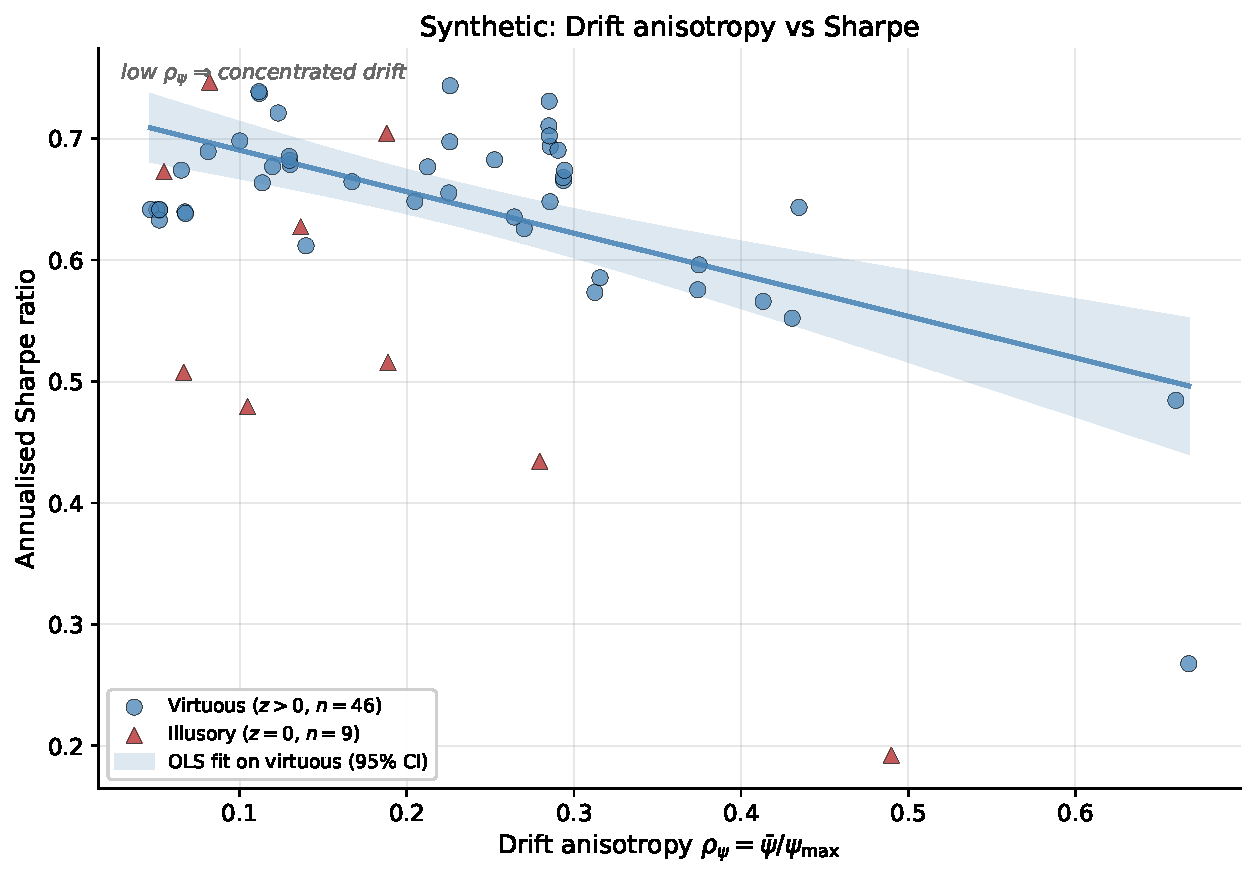
\includegraphics[width=0.78\textwidth]{fig_synth_aniso.pdf}
\caption{Drift anisotropy
$\rho_\psi = \bar\psi/\psi_{\max}$ versus annualized Sharpe ratio
across the broad grid. Each marker is one $(k,z,\tilde m)$
configuration: blue circles are the regularized regime ($z>0$, virtuous),
red triangles are the unregularized regime ($z=0$, illusory). The solid
line is an OLS fit to the virtuous configurations and the shaded band is
its 95\% confidence interval. The fitted correlation in the virtuous
regime is $r=-0.77$, matching the within-regime correlation reported in
Table~\ref{tab:sim:corr}; the all-data correlation is
$r=-0.55$.}
\label{fig:sim:aniso}
\end{figure}

Drift anisotropy is the strongest single geometric diagnostic of Sharpe in the synthetic experiments. Within the regularized regime its correlation with Sharpe is $r=-0.77$, stronger than the corresponding historical correlation of $r=-0.52$ (Section~\ref{sec:hist_data}, Figure~\ref{fig:hist:aniso}). The difference is consistent with the cleaner DGP in the simulation: empirical nonlinearities, estimation error, and structural breaks attenuate the same relationship in historical data. In both settings, the best-performing configurations combine a relatively large $\psi_{\max}$ with a small average angle $\bar\psi$. Thus, economically useful subspace adjustment is not diffuse. It is concentrated in a small number of leading directions, while most directions remain comparatively stable.

This pattern is emergent relative to the construction of the synthetic drift. The underlying Grassmann random walk is isotropic: no perturbation direction is favored ex ante. The observed anisotropy arises from the interaction between the drifting signal subspace, the finite-sample estimation problem, and the portfolio objective. Successful configurations do not simply chase all subspace motion. Instead, they filter the drift, allowing movement primarily along the directions that carry economically useful variation.

\subsubsection{Paired regime separation}
\label{sec:sim:matched}

\begin{figure}[H]
\centering
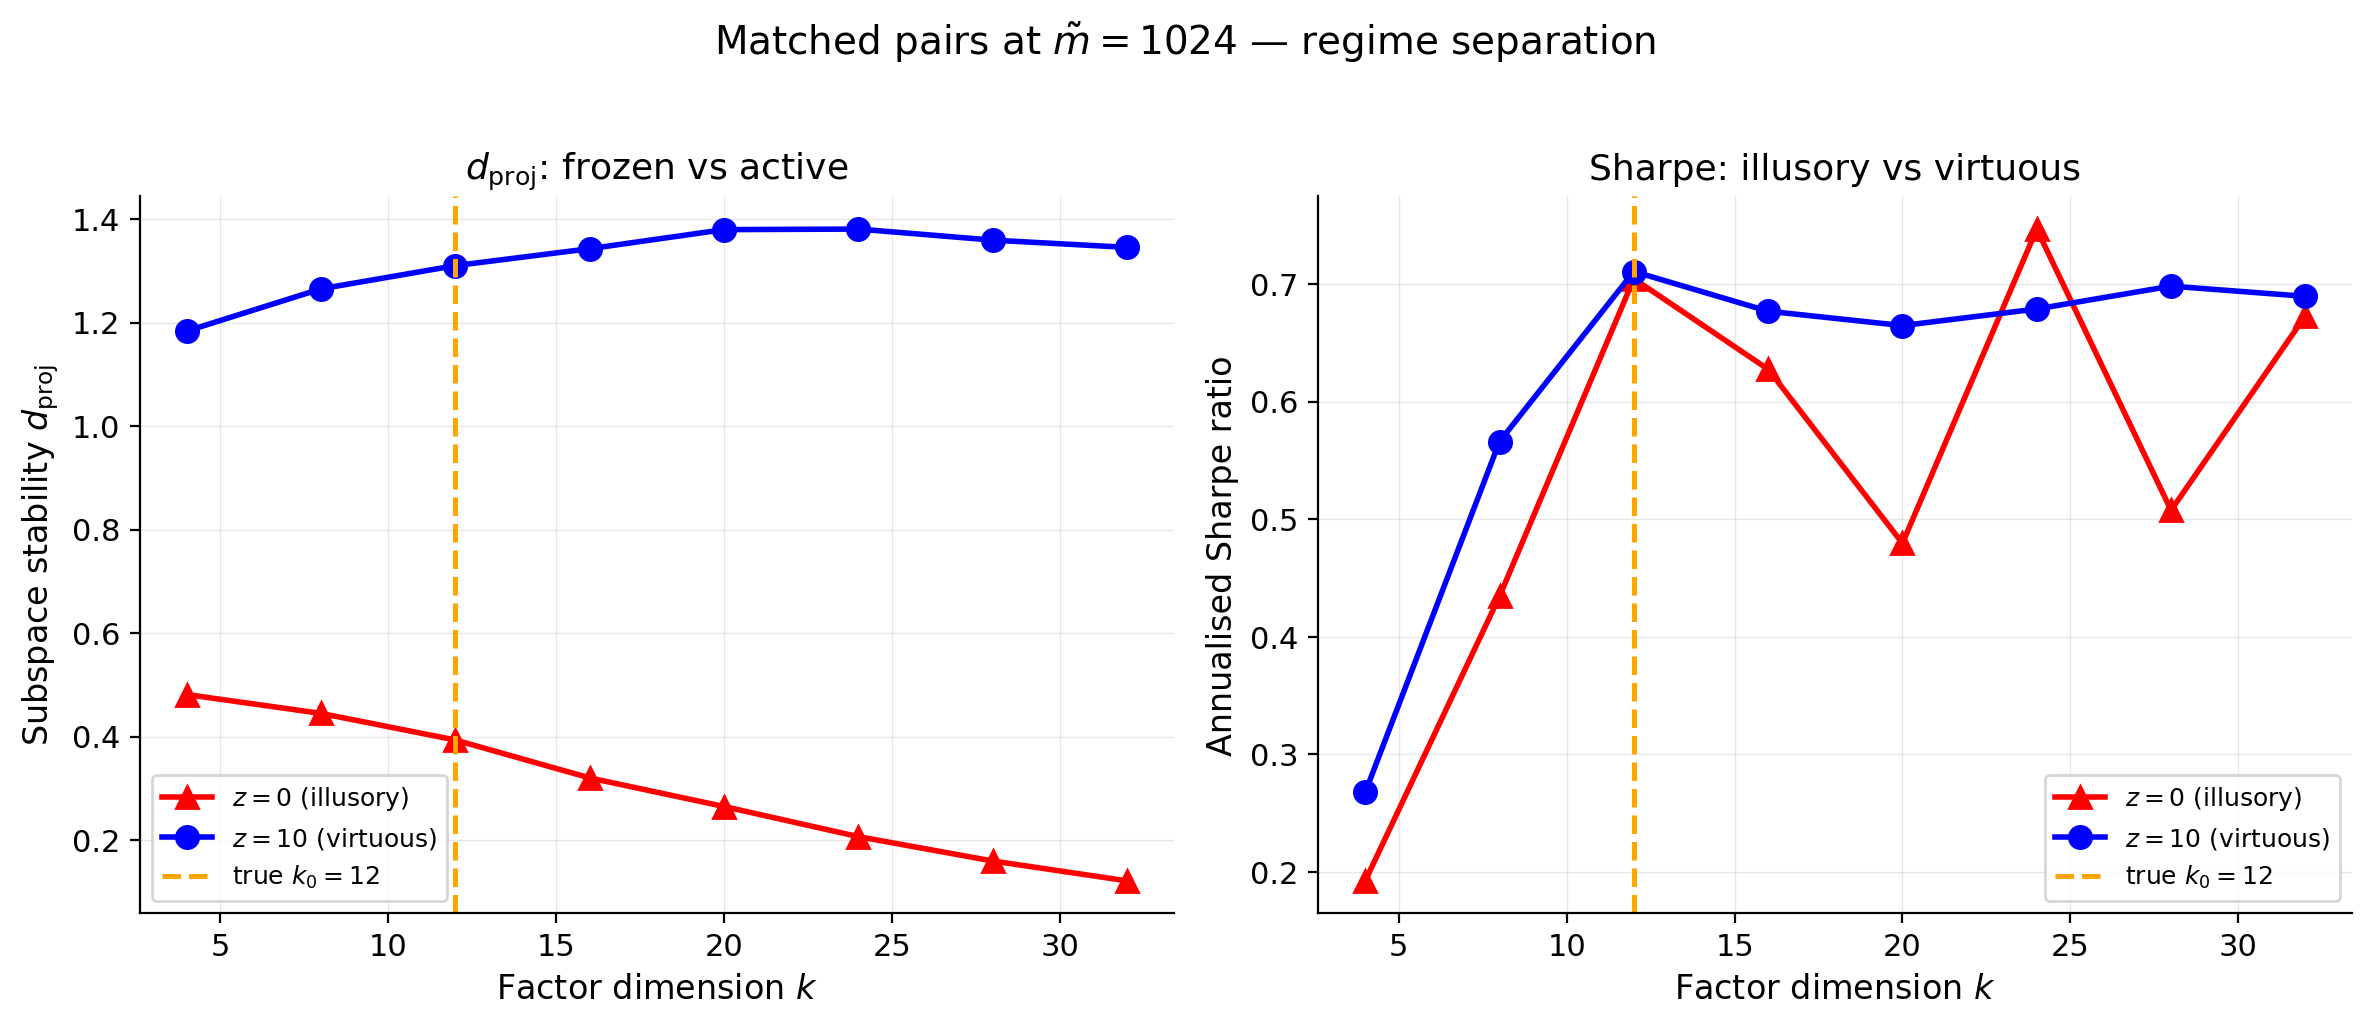
\includegraphics[width=\textwidth]{fig_p6_1.png}
\caption{Paired comparison at $\tilde m=1024$: mean projection distance
$d_{\mathrm{proj}}$ (left) and out-of-sample annualized Sharpe (right) at
$z=0$ (illusory) versus $z=10$ (virtuous), as a function of the nominal
factor dimension $k$. The orange dashed vertical line marks the true
synthetic signal rank $k_0=12$.}
\label{fig:sim:matched}
\end{figure}

The paired comparison separates the frozen and drifting regimes sharply. The synthetic $\dproj$ ratio, defined as the $z=10$ value divided by the $z=0$ value, ranges from $2.5{\times}$ at $k=4$ to $11.3{\times}$ at $k=32$. These magnitudes are quantitatively close to the historical average ratio. Moreover, the gap widens monotonically with $k$. This is exactly the qualitative behavior predicted by Theorem~\ref{thm:curv-erank}(i): as the number of noise dimensions increases, the Hessian null space at $z=0$ expands, giving the regularized estimator more directions along which it can move away from the frozen regime.

The practical implication is that $\dproj$ is best interpreted as a regime classifier rather than a within-regime performance ranker. It reliably distinguishes low-drift from high-drift configurations, but once the estimator is in the drifting regime, Sharpe depends on whether the induced subspace motion is economically aligned rather than merely large.

\subsubsection{Geometric response to increasing \texorpdfstring{$z$}{z}}
\label{sec:sim:zgrid}

\begin{figure}[H]
\centering
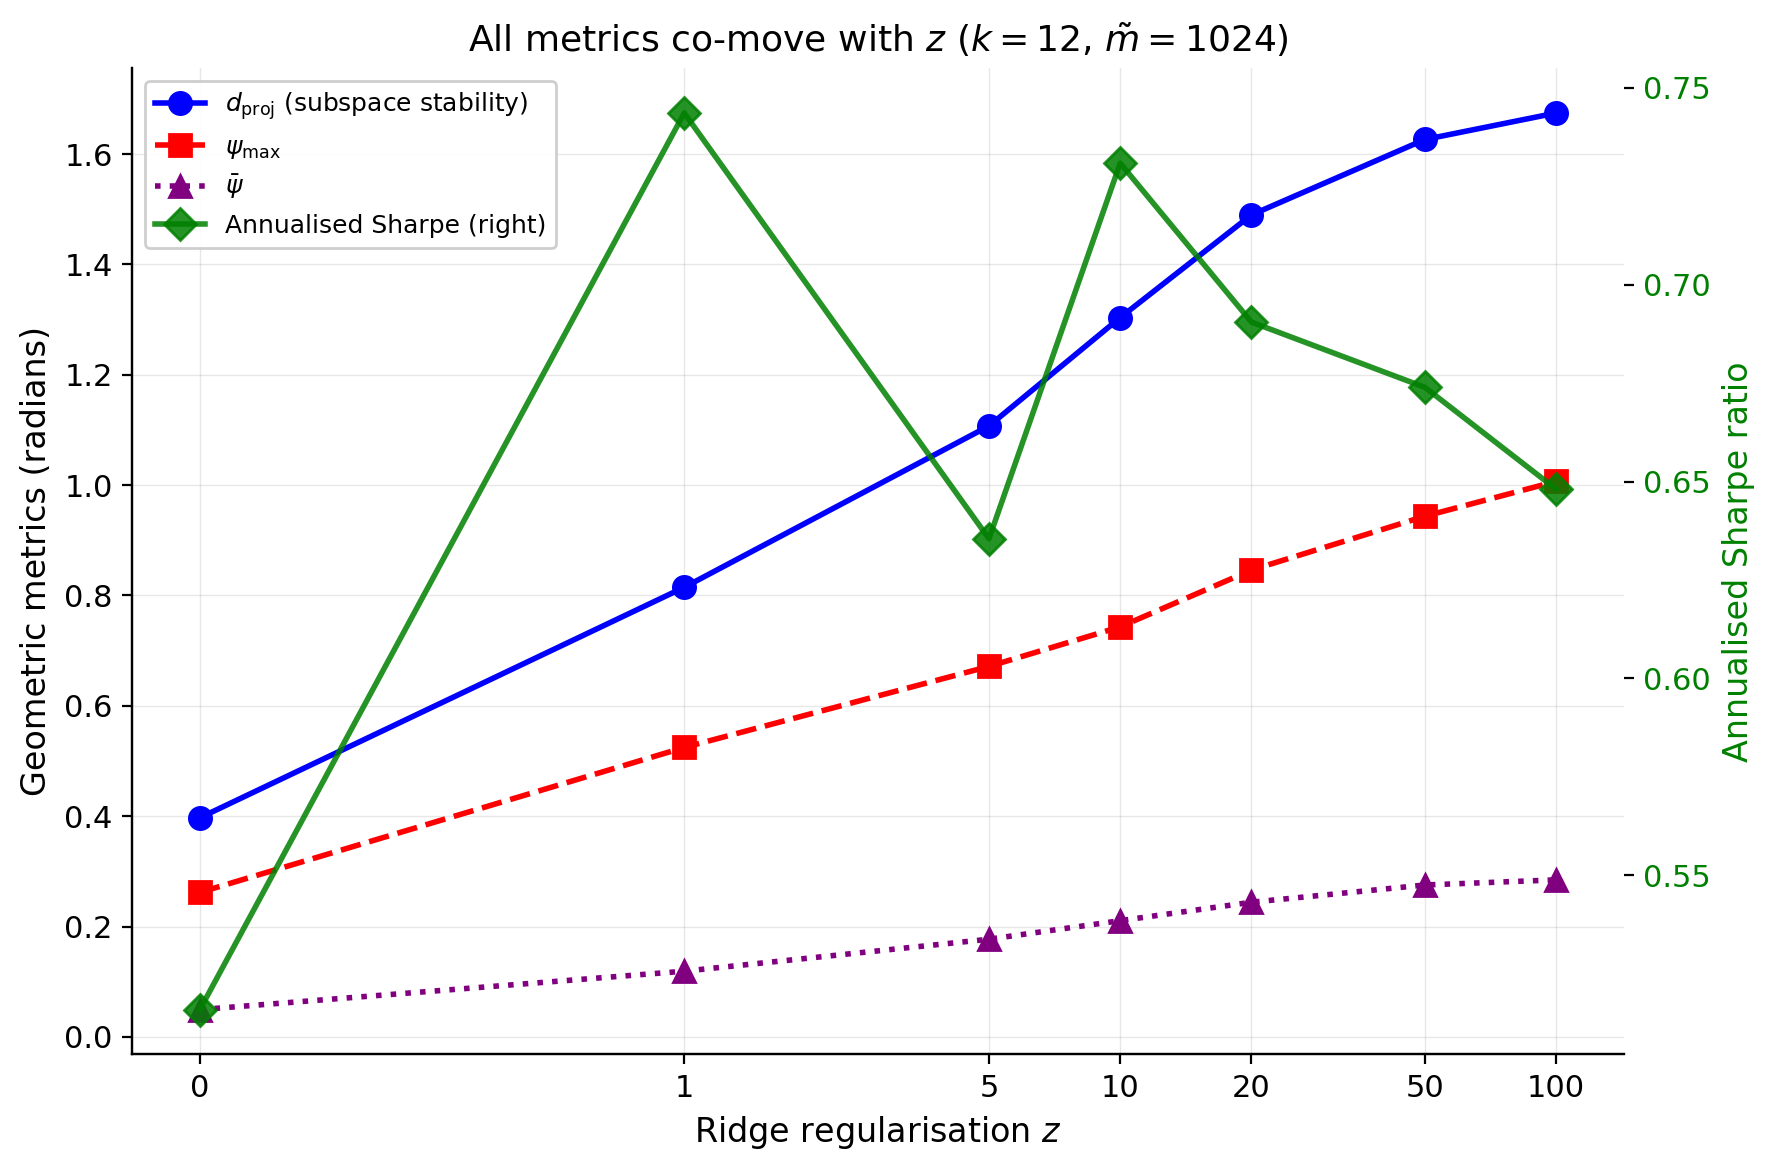
\includegraphics[width=0.78\textwidth]{fig_p3_1.png}
\caption{Geometric metrics ($d_{\mathrm{proj}}$, $\psi_{\max}$,
$\bar\psi$) on the left axis and out-of-sample annualized Sharpe ratio
on the right axis, versus the ridge regularization $z$, at $k=12$ and
$\tilde m=1024$ on a seven-point grid. All three geometric metrics rise
monotonically with $z$; in the synthetic experiment Sharpe peaks at
$z=1$ before easing back at larger $z$, in contrast to the historical
sweep where Sharpe continues to improve through high $z$.}
\label{fig:sim:zgrid}
\end{figure}

All three geometric metrics, $\dproj$, $\psi_{\max}$, and $\bar\psi$, increase monotonically with $z$, reproducing the co-movement observed in the historical data. The interesting divergence is in Sharpe. In the synthetic experiment, Sharpe peaks at $z=1$ and declines at larger $z$, whereas in the historical experiment it continues to improve through the high-$z$ range. This difference is natural. In the clean linear DGP, sufficiently strong regularization eventually over-shrinks the marginal factor direction. In the richer historical environment, by contrast, additional regularization can continue to stabilize weak but useful directions that are absent from the finite-rank simulation design.

Taken together, the broad-grid diagnostics separate three effects that are confounded in the historical data: drift strength, rank selection, and overparameterization beyond the signal space.

\subsubsection{\texorpdfstring{$z=0$}{z=0} erratic versus \texorpdfstring{$z>0$}{z>0} clean peaks}
\label{sec:sim:erratic}

\begin{figure}[H]
\centering
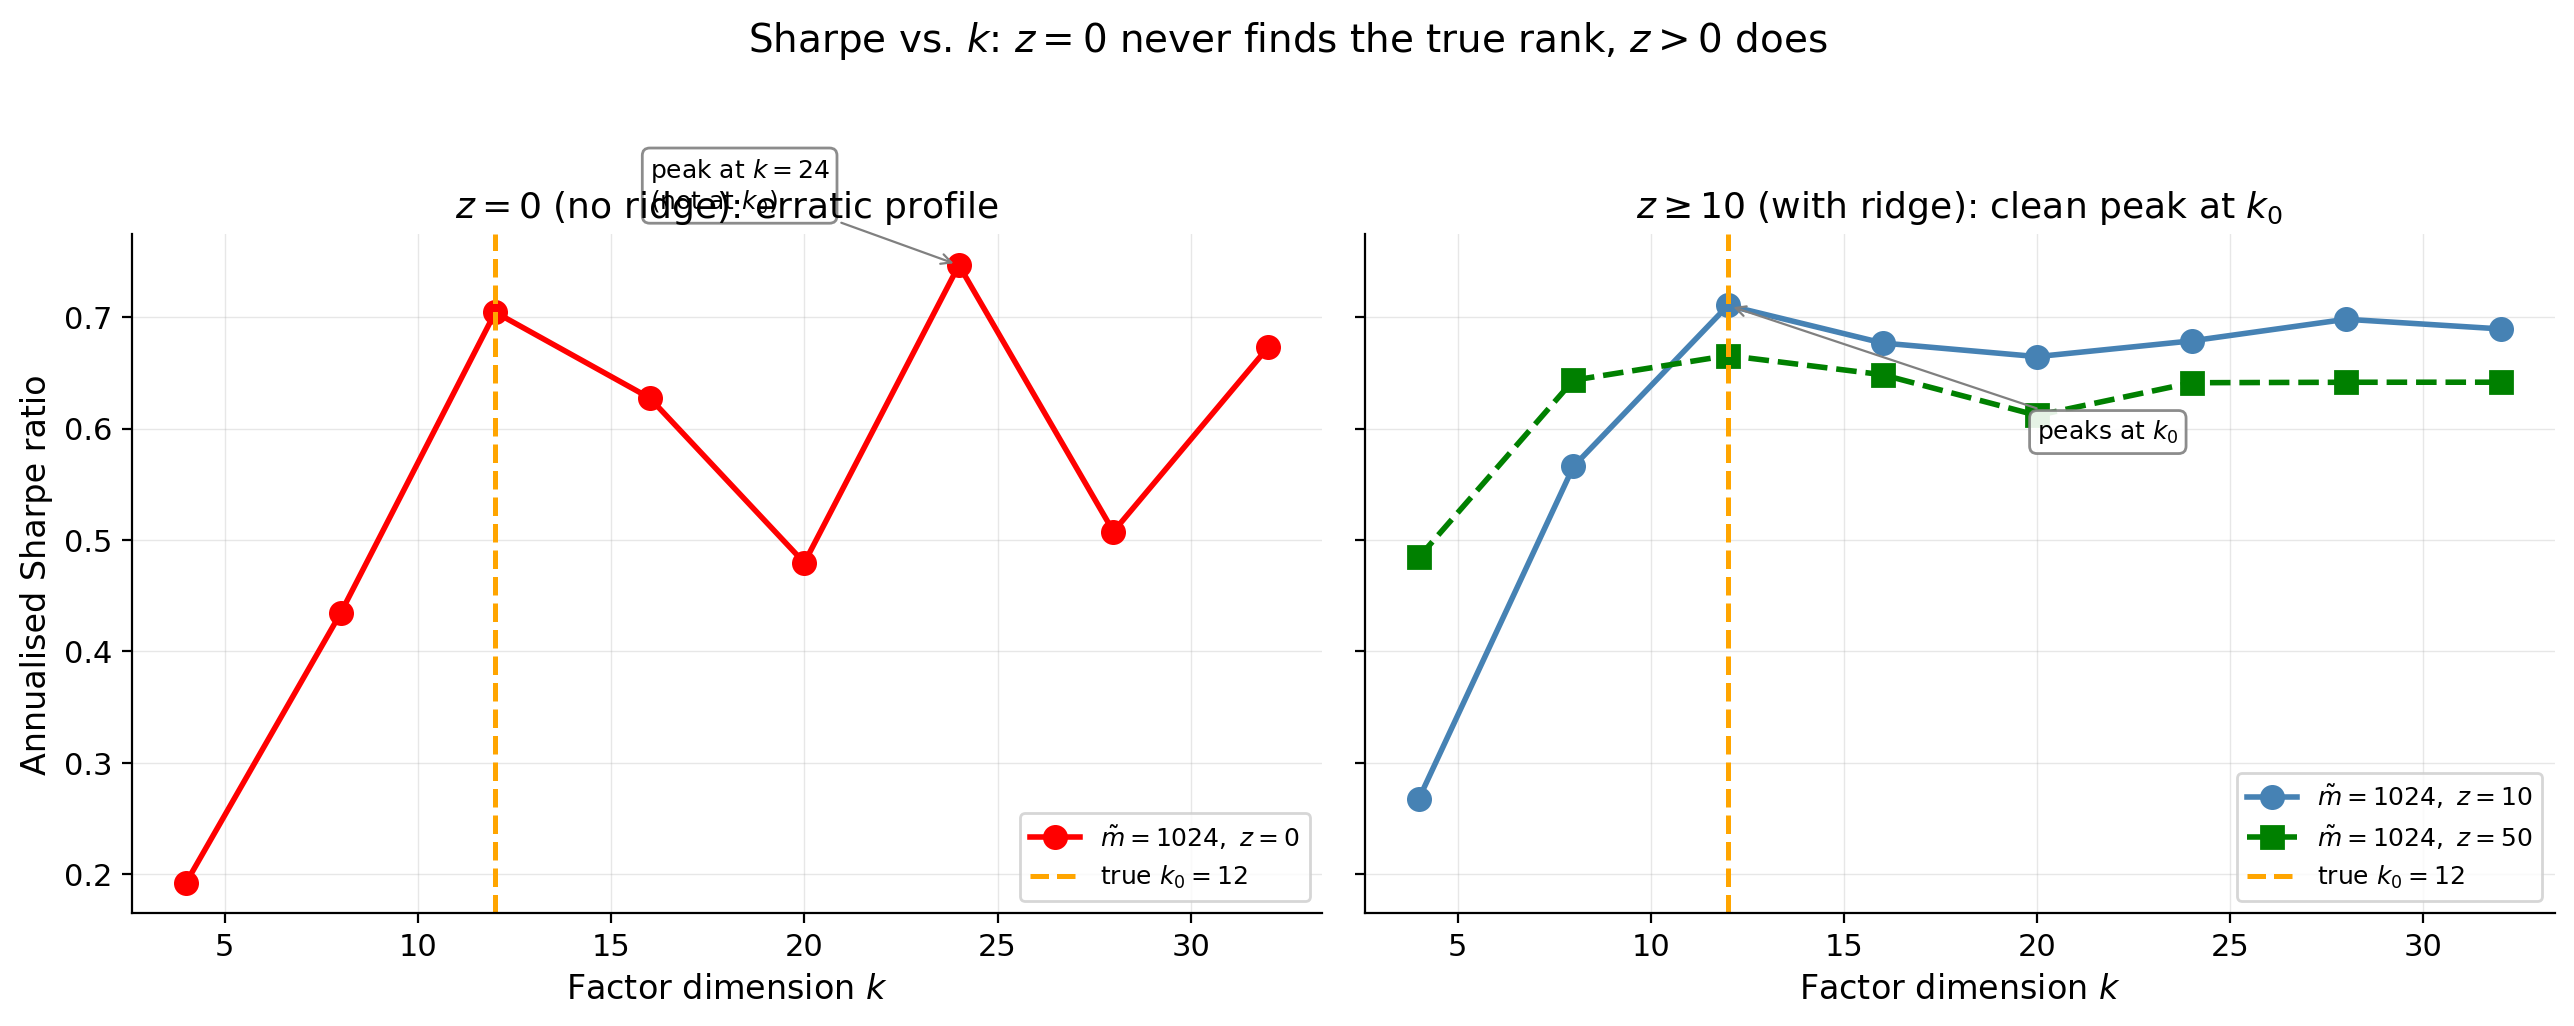
\includegraphics[width=\textwidth]{fig_p4_2.png}
\caption{Annualized Sharpe ratio versus factor dimension $k$ at
$\tilde m=1024$. Left: $z=0$ (no ridge), where the rank profile is erratic and
the apparent peak shifts to $k=16$ rather than landing at the true
signal rank. Right: $z\geq10$ (with ridge), where Sharpe peaks cleanly
at the true synthetic signal rank. The orange dashed vertical line
marks the true rank $k_0=12$ on both panels.}
\label{fig:sim:erratic}
\end{figure}

At $z=0$, the Sharpe profile is erratic and peaks at $k=16$ rather than at the true rank $k_0=12$. For $z>0$, the peak moves back to $k_0$. This is the synthetic analogue of the historical rank-selection pattern, but in a cleaner form. In the baseline historical grid, the best Sharpe configurations tend to occur just beyond the spectral cliff, a pattern we later describe as a productive illusion: mild overparameterization can appear beneficial when extra directions stabilize weak, persistent structure. In the synthetic DGP, by contrast, there is no additional
structure beyond the true rank. Once the signal space has been filled, extra directions add only noise, so the correctly regularized peak occurs exactly at $k_0$.

\subsubsection{Spectral gap cliff at \texorpdfstring{$k_0$}{k0}}
\label{sec:sim:sg}

\begin{figure}[H]
\centering
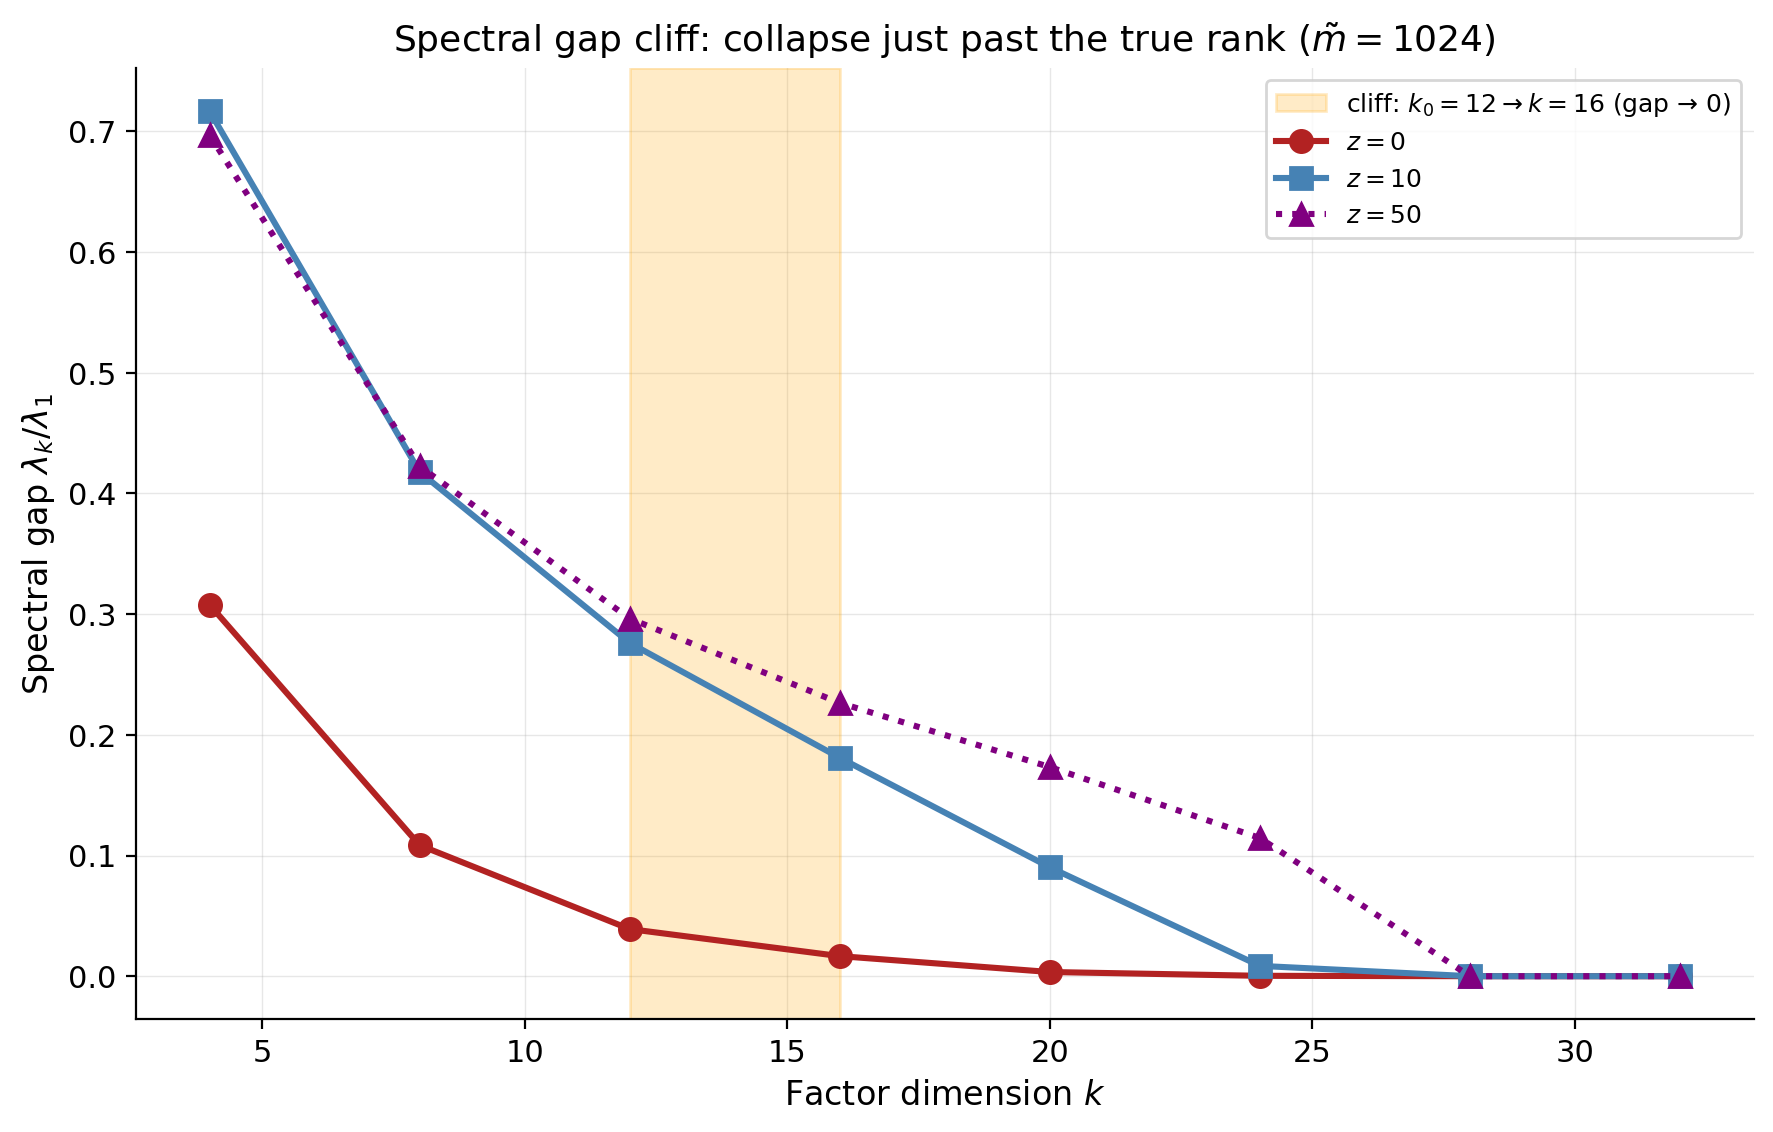
\includegraphics[width=0.78\textwidth]{fig_p2_1.png}
\caption{Spectral gap $\lambda_k/\lambda_1$ versus factor dimension $k$
at $\tilde m=1024$ for three ridge values $z\in\{0,10,50\}$. The shaded
vertical band marks the true synthetic signal rank $k_0=12$. The cliff
at $k_0$ is sharp because the synthetic DGP has an exact rank cutoff;
the regularized curves show the strongest gap, consistent with the
ridge--curvature mechanism of Theorem~\ref{thm:curv-erank}(ii).}
\label{fig:sim:sg}
\end{figure}

The spectral gap drops sharply at the true rank and then collapses for larger $k$. This is first a computational sanity check: the fitted factor covariance recovers the designed spectral cliff from finite noisy data. But it is also the finite-sample manifestation of Theorem~\ref{thm:curv-erank}(iii). Once the fitted dimension exceeds the signal dimension, the additional directions lie on the noise floor and contribute little stable variation.

\subsubsection{Effective rank collapse}
\label{sec:sim:erank}

\begin{figure}[H]
\centering
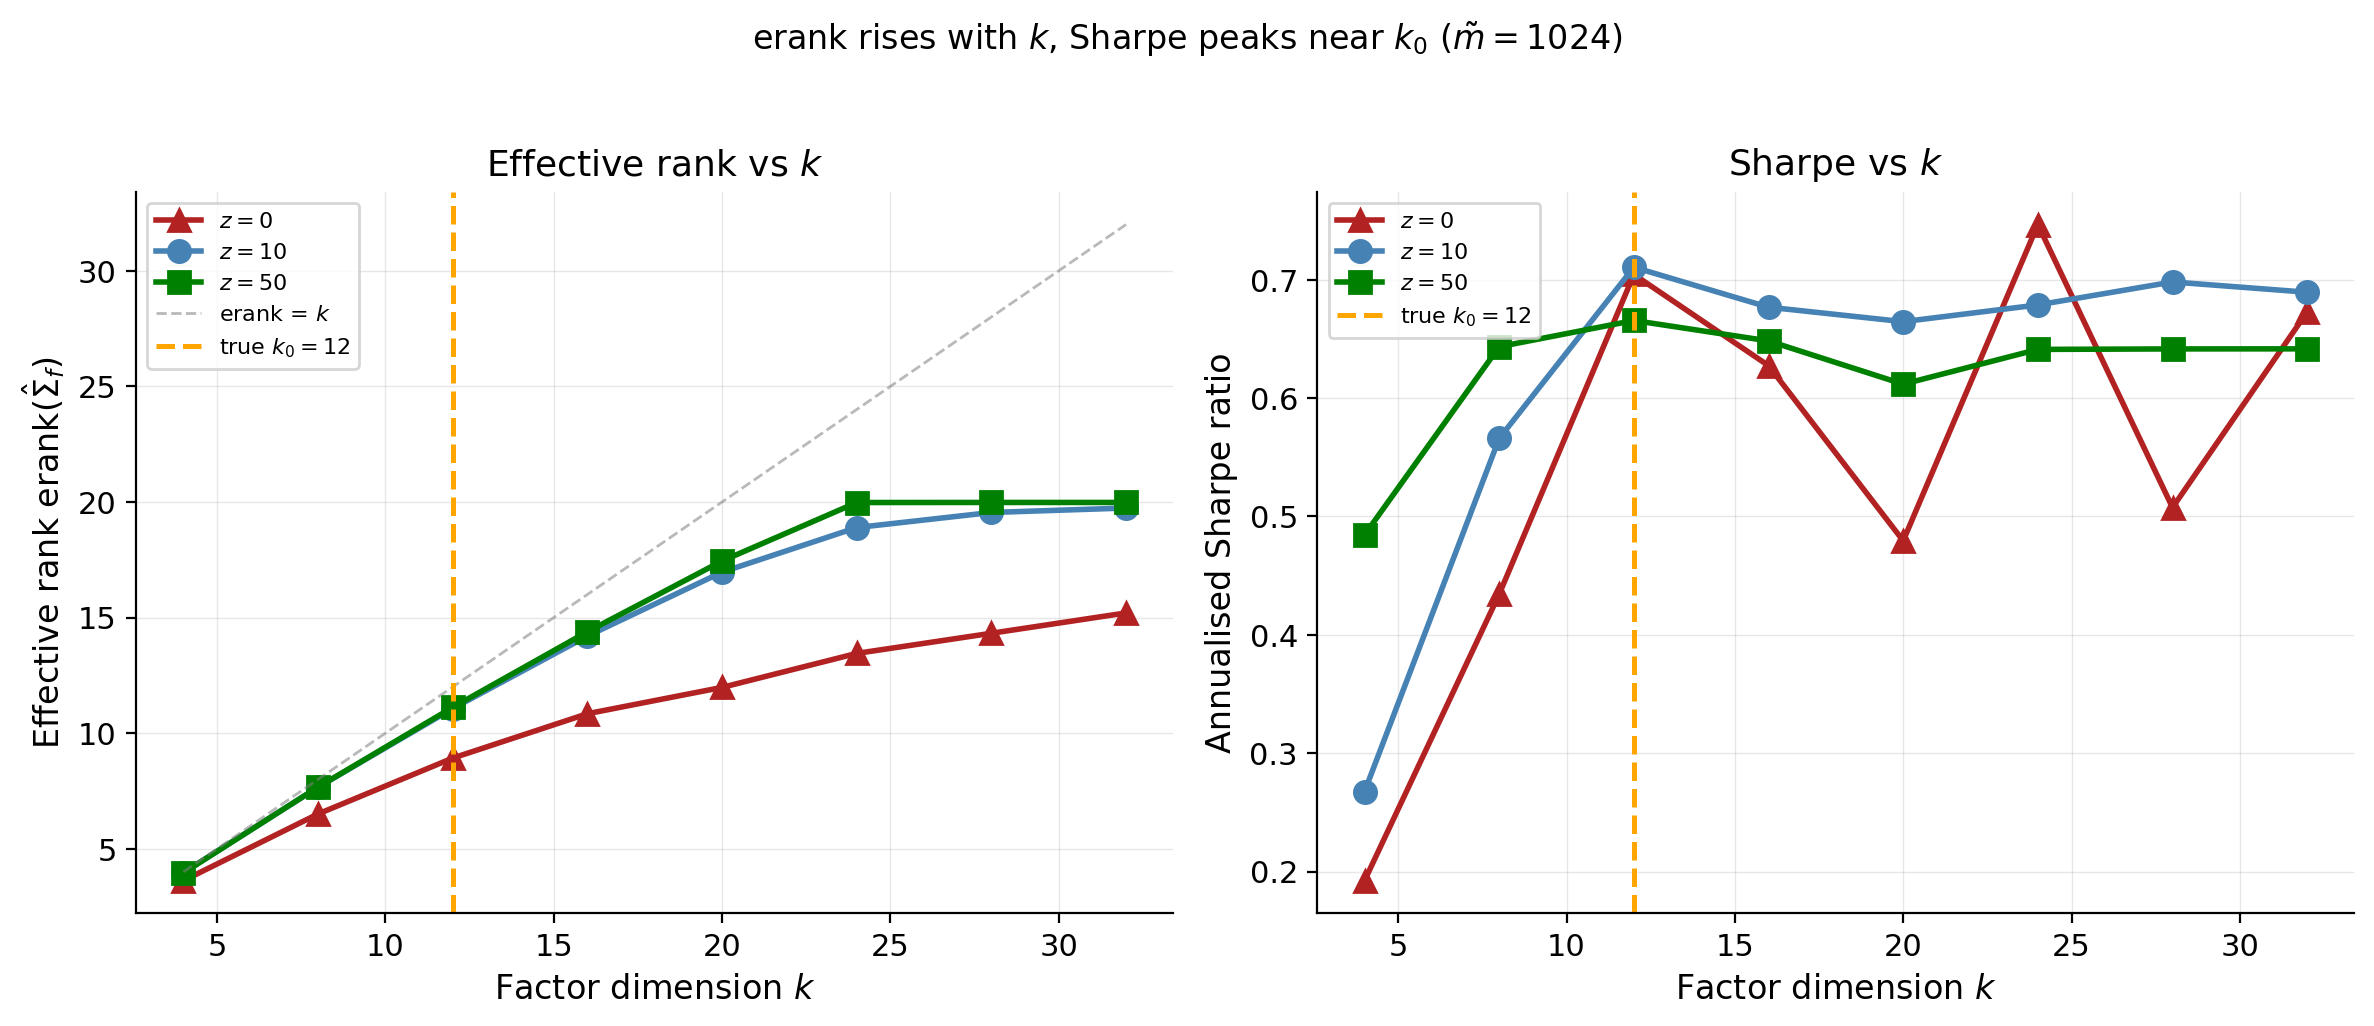
\includegraphics[width=\textwidth]{fig_p5_1.png}
\caption{Effective rank $\mathrm{erank}(\hat\Sigma_f)$ (left) and
annualized Sharpe (right) versus factor dimension $k$ at $\tilde m=1024$ for
two ridge values. The gray dashed line in the left panel is the
$\mathrm{erank}=k$ identity reference. The orange dashed vertical line
in both panels marks the true synthetic signal rank $k_0=12$. Effective
rank tracks $k$ approximately linearly for $k\leq k_0$ and saturates
beyond it; in the regularized regime, Sharpe peaks at $k_0$.}
\label{fig:sim:erank}
\end{figure}

The effective rank tracks the nominal rank approximately linearly for $k \leq k_0=12$ and then saturates. This mirrors the qualitative pattern in the historical extended backtest. Once the signal space has been filled, extra directions add only noise, so the
regularized peak is expected to occur at $k_0$, as observed. The contrast between nominal rank and effective rank is therefore central: the model becomes larger, but not meaningfully higher-dimensional in the economically relevant sense.

\subsubsection{Sharpe and \texorpdfstring{$R^2$}{R2} increase with	\texorpdfstring{$\tilde m$}{m-tilde}}
\label{sec:sim:m}

\begin{figure}[H]
\centering
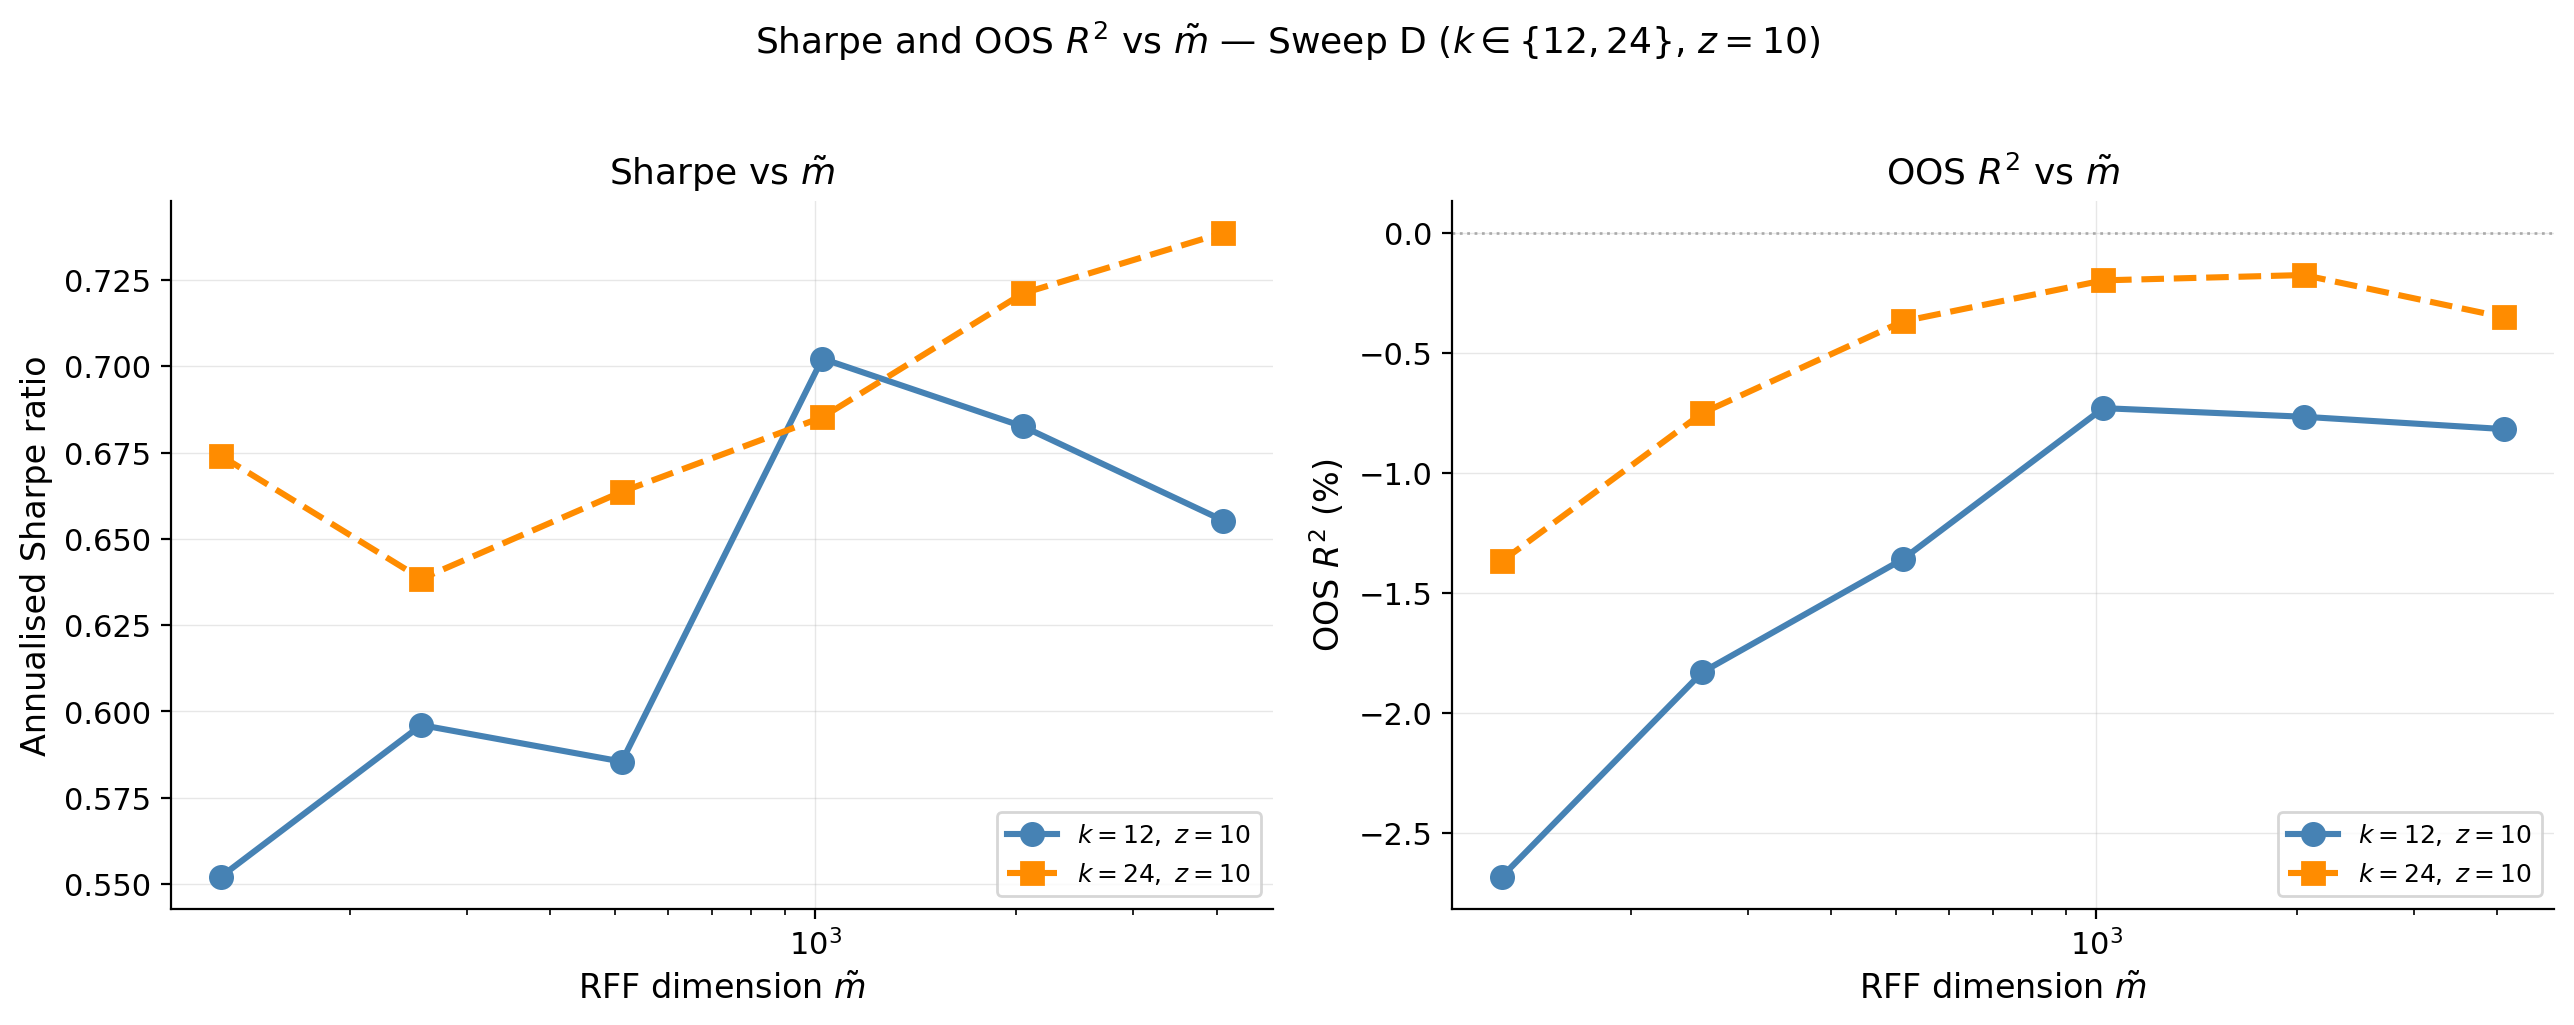
\includegraphics[width=\textwidth]{fig_sharpe_r2_smooth.png}
\caption{Annualized Sharpe ratio (left) and out-of-sample $R^2$ in
percent (right) versus the RFF dimension $\tilde m$ at fixed
$z=10$, averaged across RFF seeds, for two factor dimensions
$k\in\{12,24\}$. Sharpe rises visibly with $\tilde m$, while OOS $R^2$ rises
modestly and stays near zero in absolute terms; the portfolio metric
benefits more from added complexity than the predictive metric does.}
\label{fig:sim:m}
\end{figure}

At $k=24$ and $z=10$, Sharpe rises from about $0.67$ to $0.73$ as $\tilde m$ grows from $128$ to $4096$. Over the same range, $R^2$ improves from
roughly $-0.014$ to $-0.004$. The predictive fit therefore improves only modestly and remains weak in absolute terms, while the portfolio metric improves more visibly. This is consistent with the central empirical message of the paper: small improvements in the stability and alignment of weak predictive signals can matter more for portfolio performance than large gains in cross-sectional explanatory power.

The result also clarifies the role of the RFF lift. Because the synthetic DGP is linear, increasing $\tilde m$ does not uncover additional nonlinear signal by design. Instead, the overcomplete feature representation, combined with regularization, appears to improve the finite-sample conditioning of the estimated signal subspace. This is consistent with the KMZ interpretation that overparameterization can deliver useful implicit regularization even when the underlying signal is low-dimensional.

\subsection{Correlation landscape}
\label{sec:sim:corr}

\begin{table}[H]
\centering
\caption{Metric--Sharpe correlations in the synthetic experiments.
Historical values from Section~\ref{sec:hist_data} are shown in parentheses
where directly comparable. Note that the synthetic anisotropy correlation
of $-0.77$ cited in Section~\ref{sec:sim:aniso} and Figure~\ref{fig:sim:aniso}
refers to the within-virtuous-regime column; the all-data anisotropy
correlation is $-0.55$.}
\label{tab:sim:corr}
\smallskip
\begin{tabular}{lcc}
\toprule
Metric & All data & Virtuous regime ($z>0$) \\
\midrule
$\dproj$           & $+0.41\ (+0.23)$  & $-0.04\ (-0.07)$ \\
$\psi_{\max}$    & $+0.45$           & $+0.20$          \\
$-\bar\psi$      & $+0.20$           & $+0.71\ (+0.47)$ \\
$\erank$           & $+0.61$           & $+0.63$          \\
$-\mathrm{sg}$     & $+0.45$           & $+0.81$          \\
$\rho_\psi$      & $-0.55\ (-0.52)$  & $-0.77\ (-0.52)$ \\
\bottomrule
\end{tabular}
\end{table}

The structural pattern matches the historical correlation landscape. Projection distance $\dproj$ is useful primarily as a regime classifier: it separates frozen from drifting configurations, but has little within-regime ranking power. Anisotropy dominates within the regularized regime, indicating that Sharpe is highest when subspace motion is concentrated rather than diffuse. The spectral gap is informative about the signal-space boundary, but is not by itself a full performance-ranking device.

The one important divergence from the historical results is the absence of a productive illusion in the clean DGP. In the historical data, peak Sharpe occurs just beyond the spectral cliff. In the broad synthetic exercise, by contrast, peak Sharpe occurs at the true signal rank. This divergence is expected: the clean DGP contains no structure beyond $k_0$ for overparameterization to exploit. The empirical productive illusion therefore appears to be tied to genuine economic complexity; weak nonlinearities, persistent omitted directions, or slowly rotating signals; rather than to a mechanical artifact of the estimator.

\subsection{Short-window rank-aligned extension around the interpolation boundary}
\label{sec:sim:shortwindow}

The broad-grid synthetic study validates the main geometric mechanisms in a controlled long-window environment. We now add a shorter-window extension in which the interpolation threshold $\tilde m/T=1$ is visible on the experimental grid. The goal is not to restate the long-window results, but to check whether the same diagnostics remain useful when the estimator has less time-series information and the RFF dictionary becomes large relative to the training sample. The underlying synthetic rank is fixed at $k_0=18$. We compare three runs: a slightly rank-constrained fit with $(k,T)=(17,24)$, a rank-aligned fit with $(k,T)=(18,24)$, and a longer rank-aligned fit with $(k,T)=(18,36)$. In each case, feature complexity is varied through the number of RFF components $\tilde m$.

These experiments ask a narrower question than the broad-grid analysis. The issue is not whether every finite-sample curve is monotone; they are not; but whether, near and beyond the interpolation boundary, richer feature lifts improve out-of-sample behavior without degrading the internal geometry of the fitted representation. Because the window length and grid differ from the broad-grid runs, the Sharpe levels should be read as within-experiment comparisons rather than as directly comparable performance numbers. The point is the geometry-performance relation around the interpolation boundary.

This setup also makes contact with the double-descent intuition in the virtue-of-complexity literature \cite{KMZ24,KM25}. Because the grid visibly crosses the interpolation threshold, the dashed boundary in the figures should be read as a stress point rather than as a terminal limit: performance need not improve smoothly at the threshold itself, but can recover and strengthen again once the model moves into the overparameterized region with sufficient regularization and with a fitted rank that remains well aligned with the underlying signal.

\begin{table}[H]
\centering
\caption{Headline comparison for the three short-window synthetic runs. ``Best tail'' refers to the best average OOS $R^2$ attained in the high-complexity tail.}
\label{tab:sim:shortheadline}
\scriptsize
\setlength{\tabcolsep}{4pt}
\begin{adjustbox}{max width=\textwidth}
\begin{tabular}{lrrrrrrrr}
\toprule
Run & Baseline $R^2$ & Best-tail $R^2$ & Baseline Sharpe & Max Sharpe & Baseline $\erank$ & Tail $\erank$ & Baseline gap & Tail gap \\
\midrule
$k=17,\ T=24$ & $-0.0027$ & $0.0007$ & $0.436$ & $0.873$ & $15.488$ & $16.824$ & $0.224$ & $0.555$ \\
$k=18,\ T=24$ & $-0.0028$ & $0.0010$ & $0.417$ & $0.836$ & $16.214$ & $17.801$ & $0.200$ & $0.542$ \\
$k=18,\ T=36$ & $-0.0021$ & $0.0016$ & $0.400$ & $0.920$ & $16.776$ & $17.830$ & $0.277$ & $0.566$ \\
\bottomrule
\end{tabular}
\end{adjustbox}
\end{table}

Table~\ref{tab:sim:shortheadline} shows the broad pattern. In all three runs, the linear baseline is economically and geometrically weaker than the high-complexity tail. Aligning the fitted rank with the true synthetic rank improves the picture at
$T=24$: the far-right tail becomes uniformly positive in average out-of-sample $R^2$, while effective rank moves much closer to the underlying rank~18. Lengthening the window from $T=24$ to $T=36$ strengthens the relation again: the positive tail begins earlier, peaks higher, and is accompanied by still stronger effective-rank and gap-ratio behavior.

\begin{figure}[H]
\centering
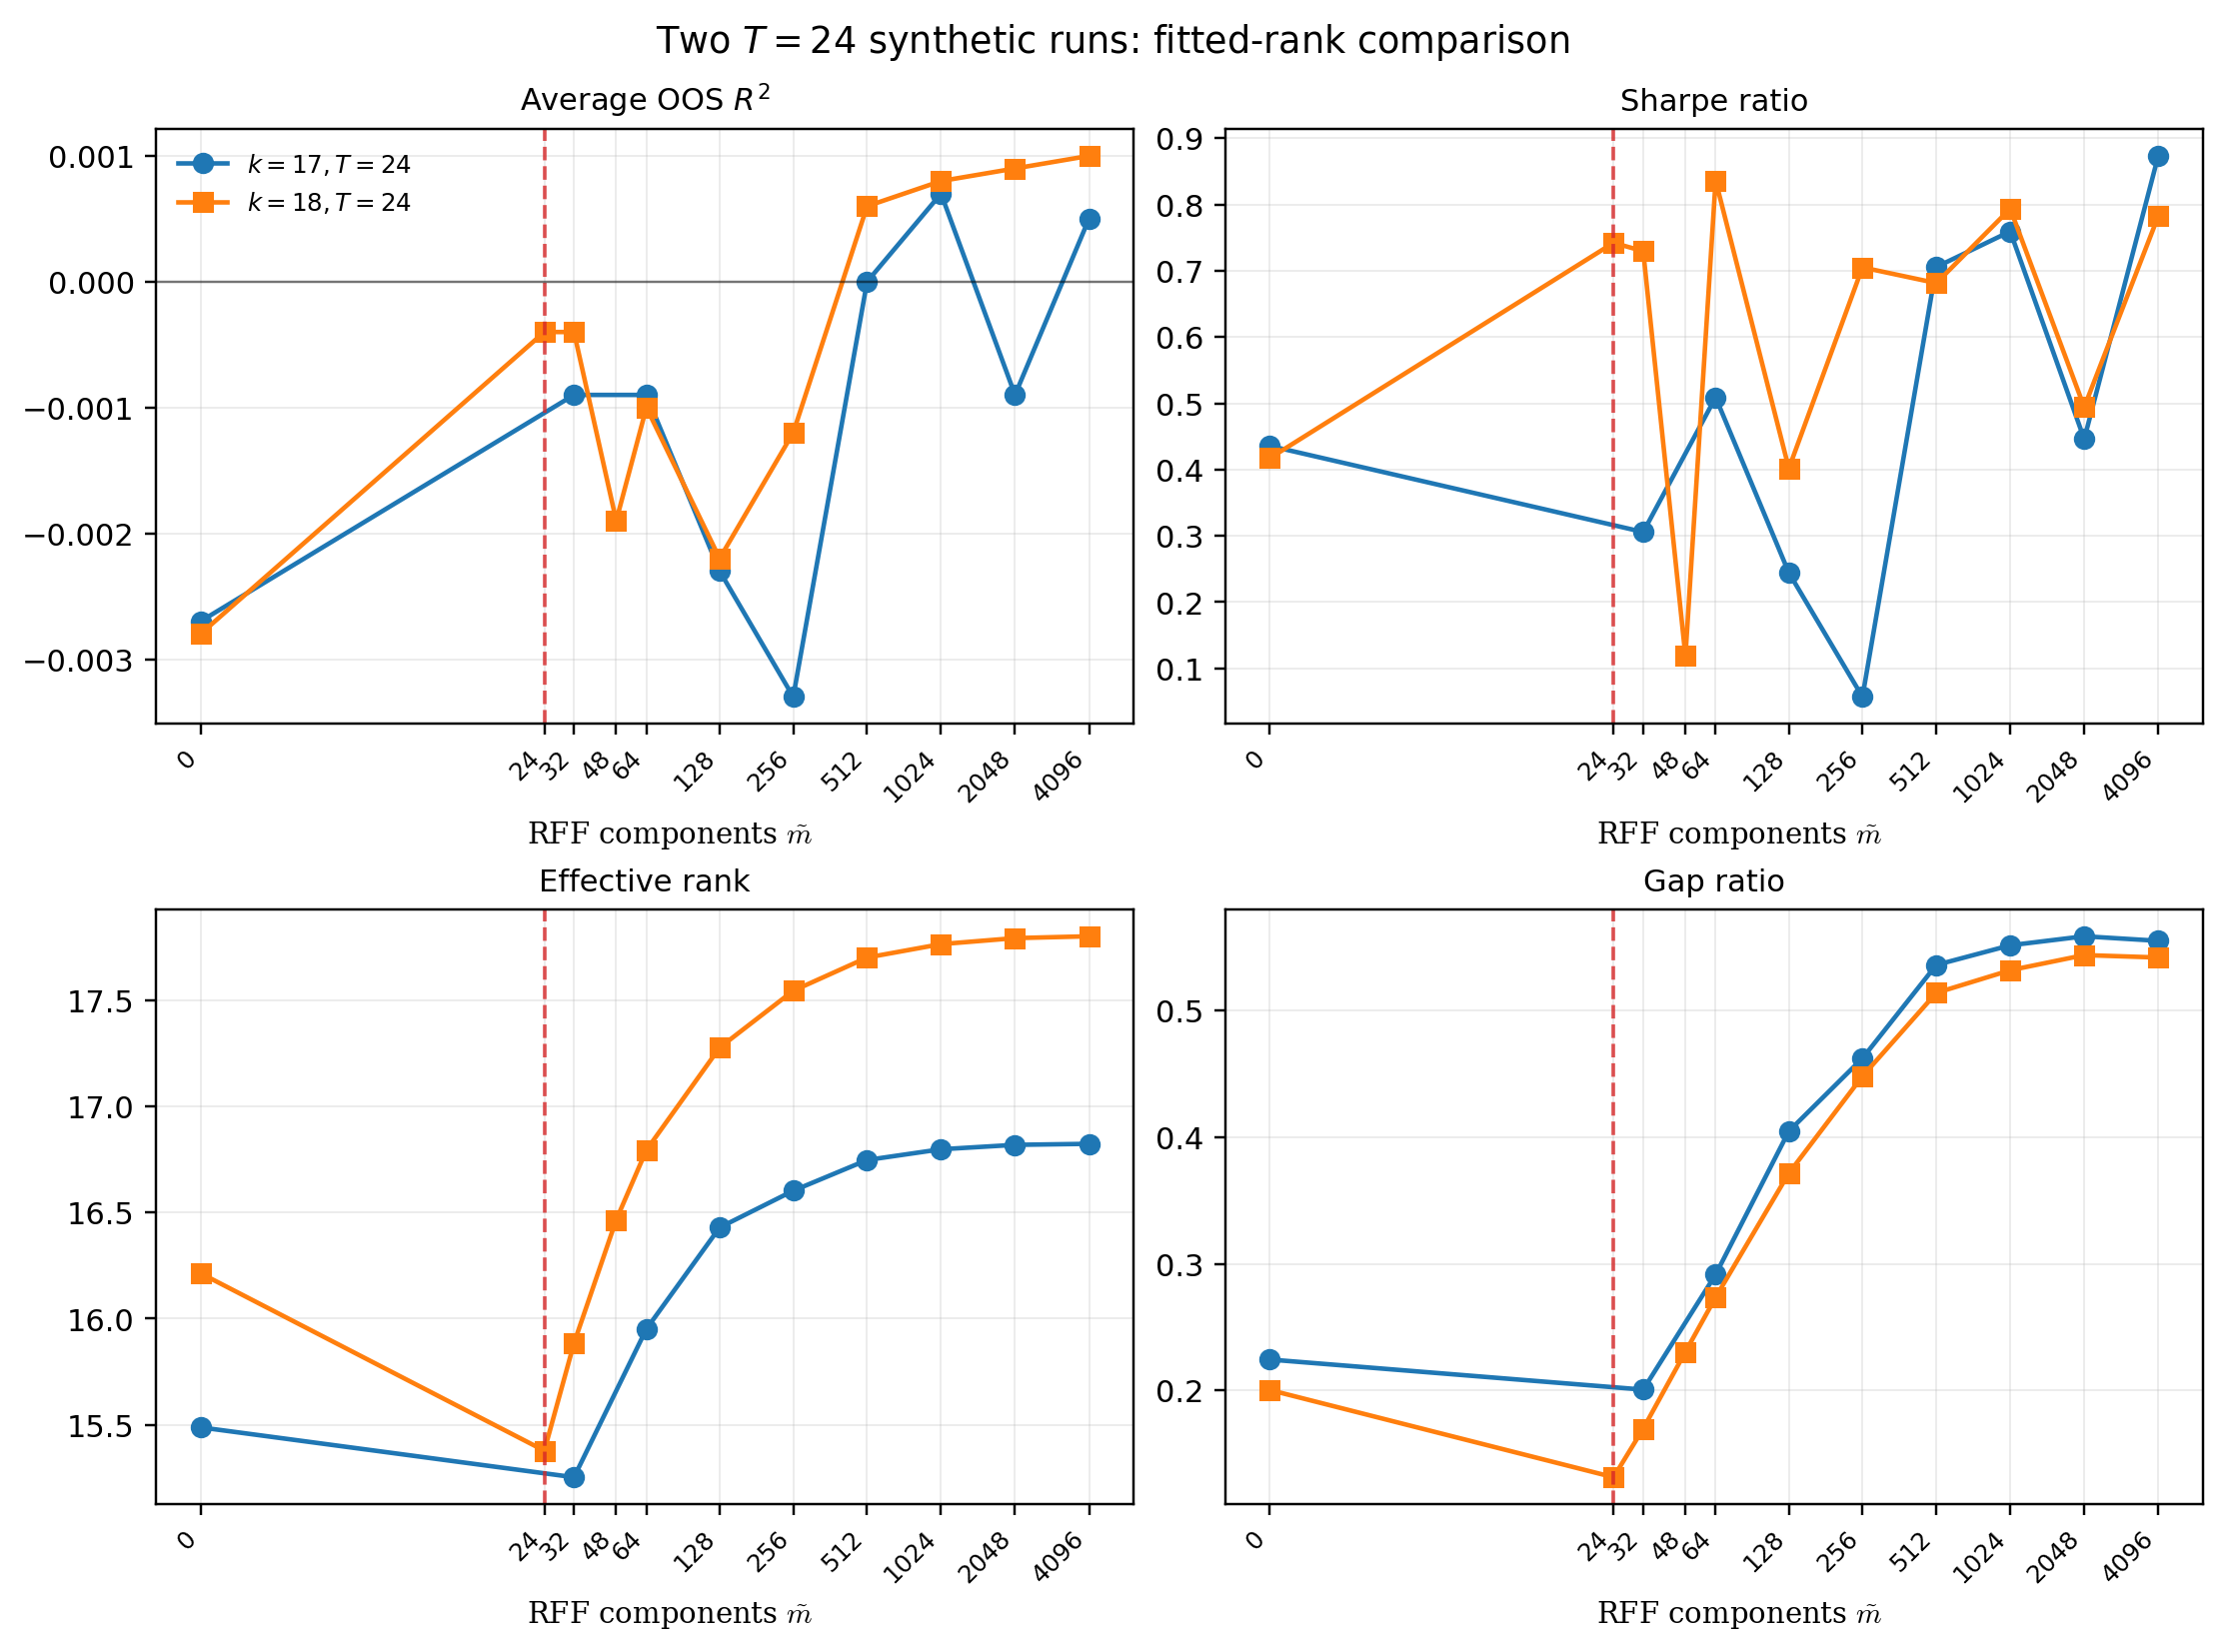
\includegraphics[width=0.97\linewidth]{synth_v5_main_compare.png}
\caption{Two $T=24$ runs: fitted-rank comparison across average out-of-sample $R^2$, Sharpe ratio, effective rank, and gap ratio. The dashed vertical line marks $\tilde m/T=1$ at $\tilde m=24$.}
\label{fig:sim:main24}
\end{figure}

Figure~\ref{fig:sim:main24} reports the two $T=24$ specifications. The curves are finite-sample objects, so the relevant comparison is not monotonicity at every point but the behavior near and beyond the interpolation threshold. When the fitted rank is aligned with the synthetic rank, the out-of-sample $R^2$ curve improves sharply at the boundary and the far-right tail is entirely positive. The Sharpe panel tells the same qualitative story: both runs improve over the linear baseline in the high-complexity region, but the rank-aligned specification extracts that benefit earlier and more consistently.

The lower panels matter for the geometry story. In the $k=17$ run, $\erank$ rises from $15.488$ to about $16.824$ and then plateaus below the nominal dimension. In the rank-aligned $k=18$ run, $\erank$ rises from $16.214$ to about $17.801$, much closer to the underlying synthetic rank. Gap ratio behaves similarly: after a softer value at the boundary, it climbs steadily toward roughly $0.54$, matching the strong tail behavior of the rank-constrained fit while doing so under the correctly specified fitted rank.

\begin{figure}[H]
\centering
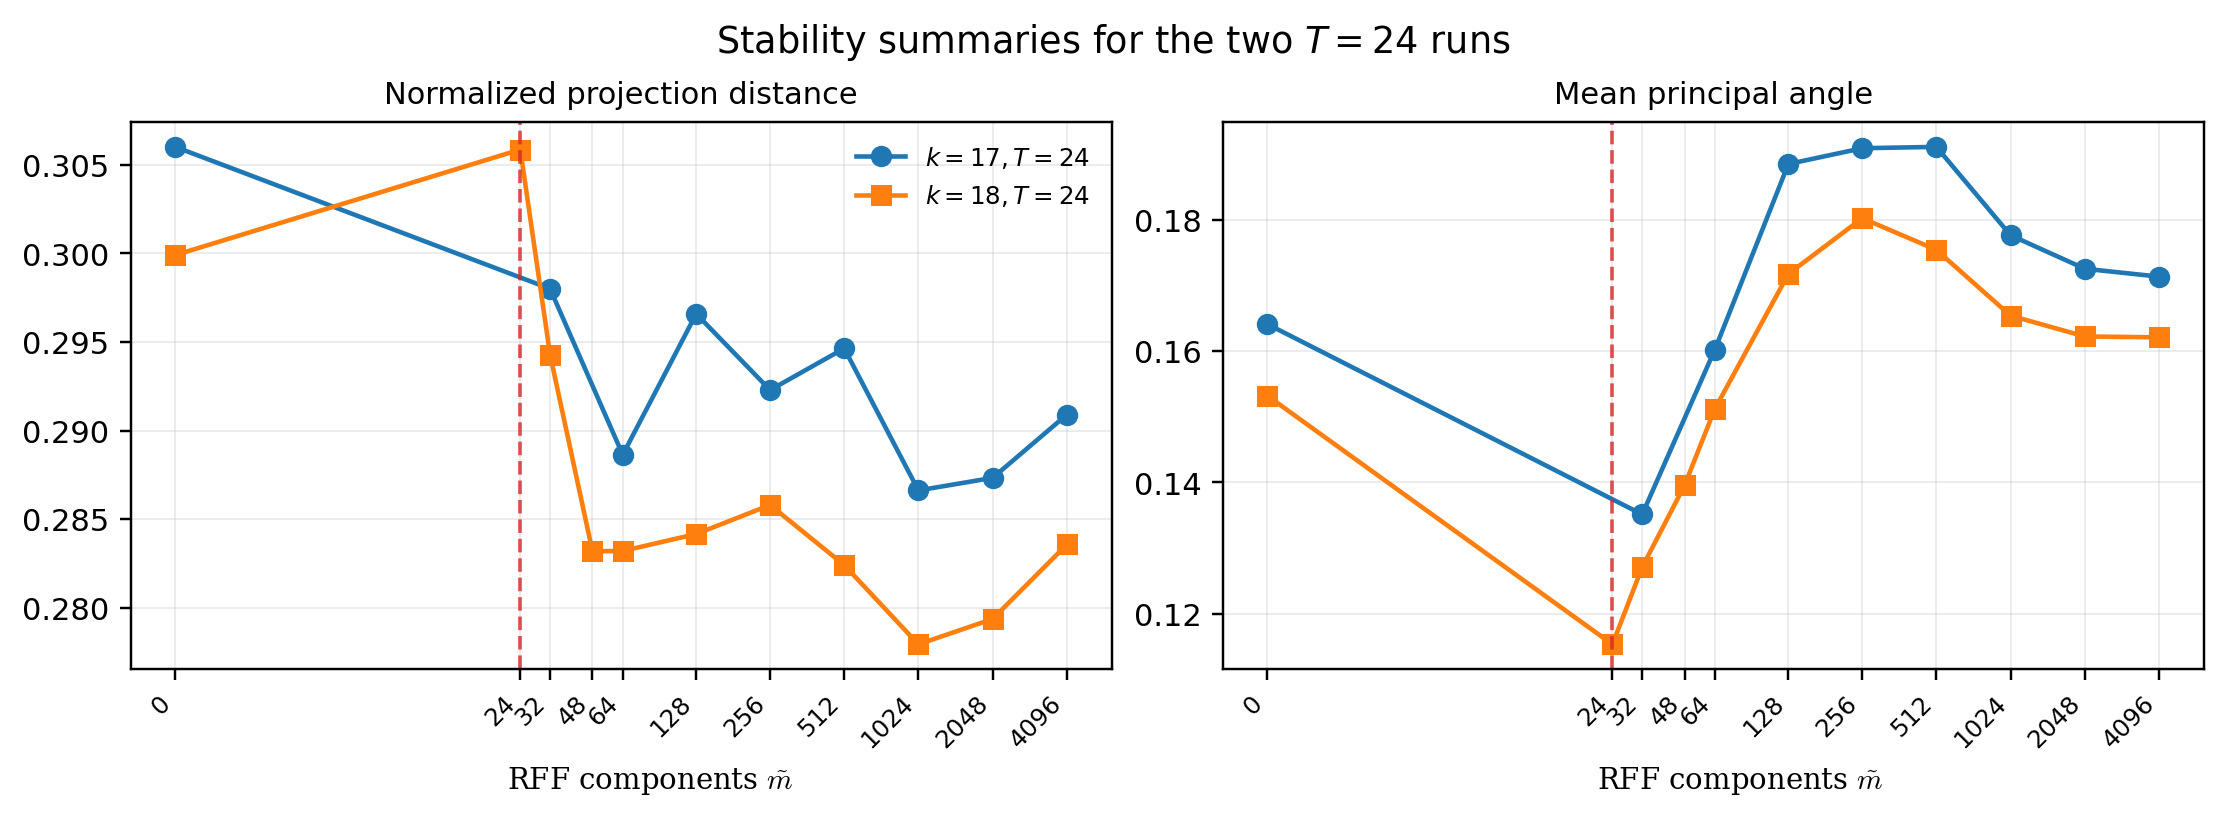
\includegraphics[width=0.97\linewidth]{synth_v5_stability_compare.png}
\caption{Stability summaries for the two $T=24$ runs. The dashed vertical line marks $\tilde m/T=1$ at $\tilde m=24$.}
\label{fig:sim:stability24}
\end{figure}

The stability comparison is equally useful. Normalized projection distance and mean principal angle do rise as the lift moves away from the boundary, but the high-complexity tail does not exhibit geometric blow-up. The rank-aligned specification improves fit and structural concentration without paying for it through visibly uncontrolled subspace motion.

\begin{figure}[H]
\centering
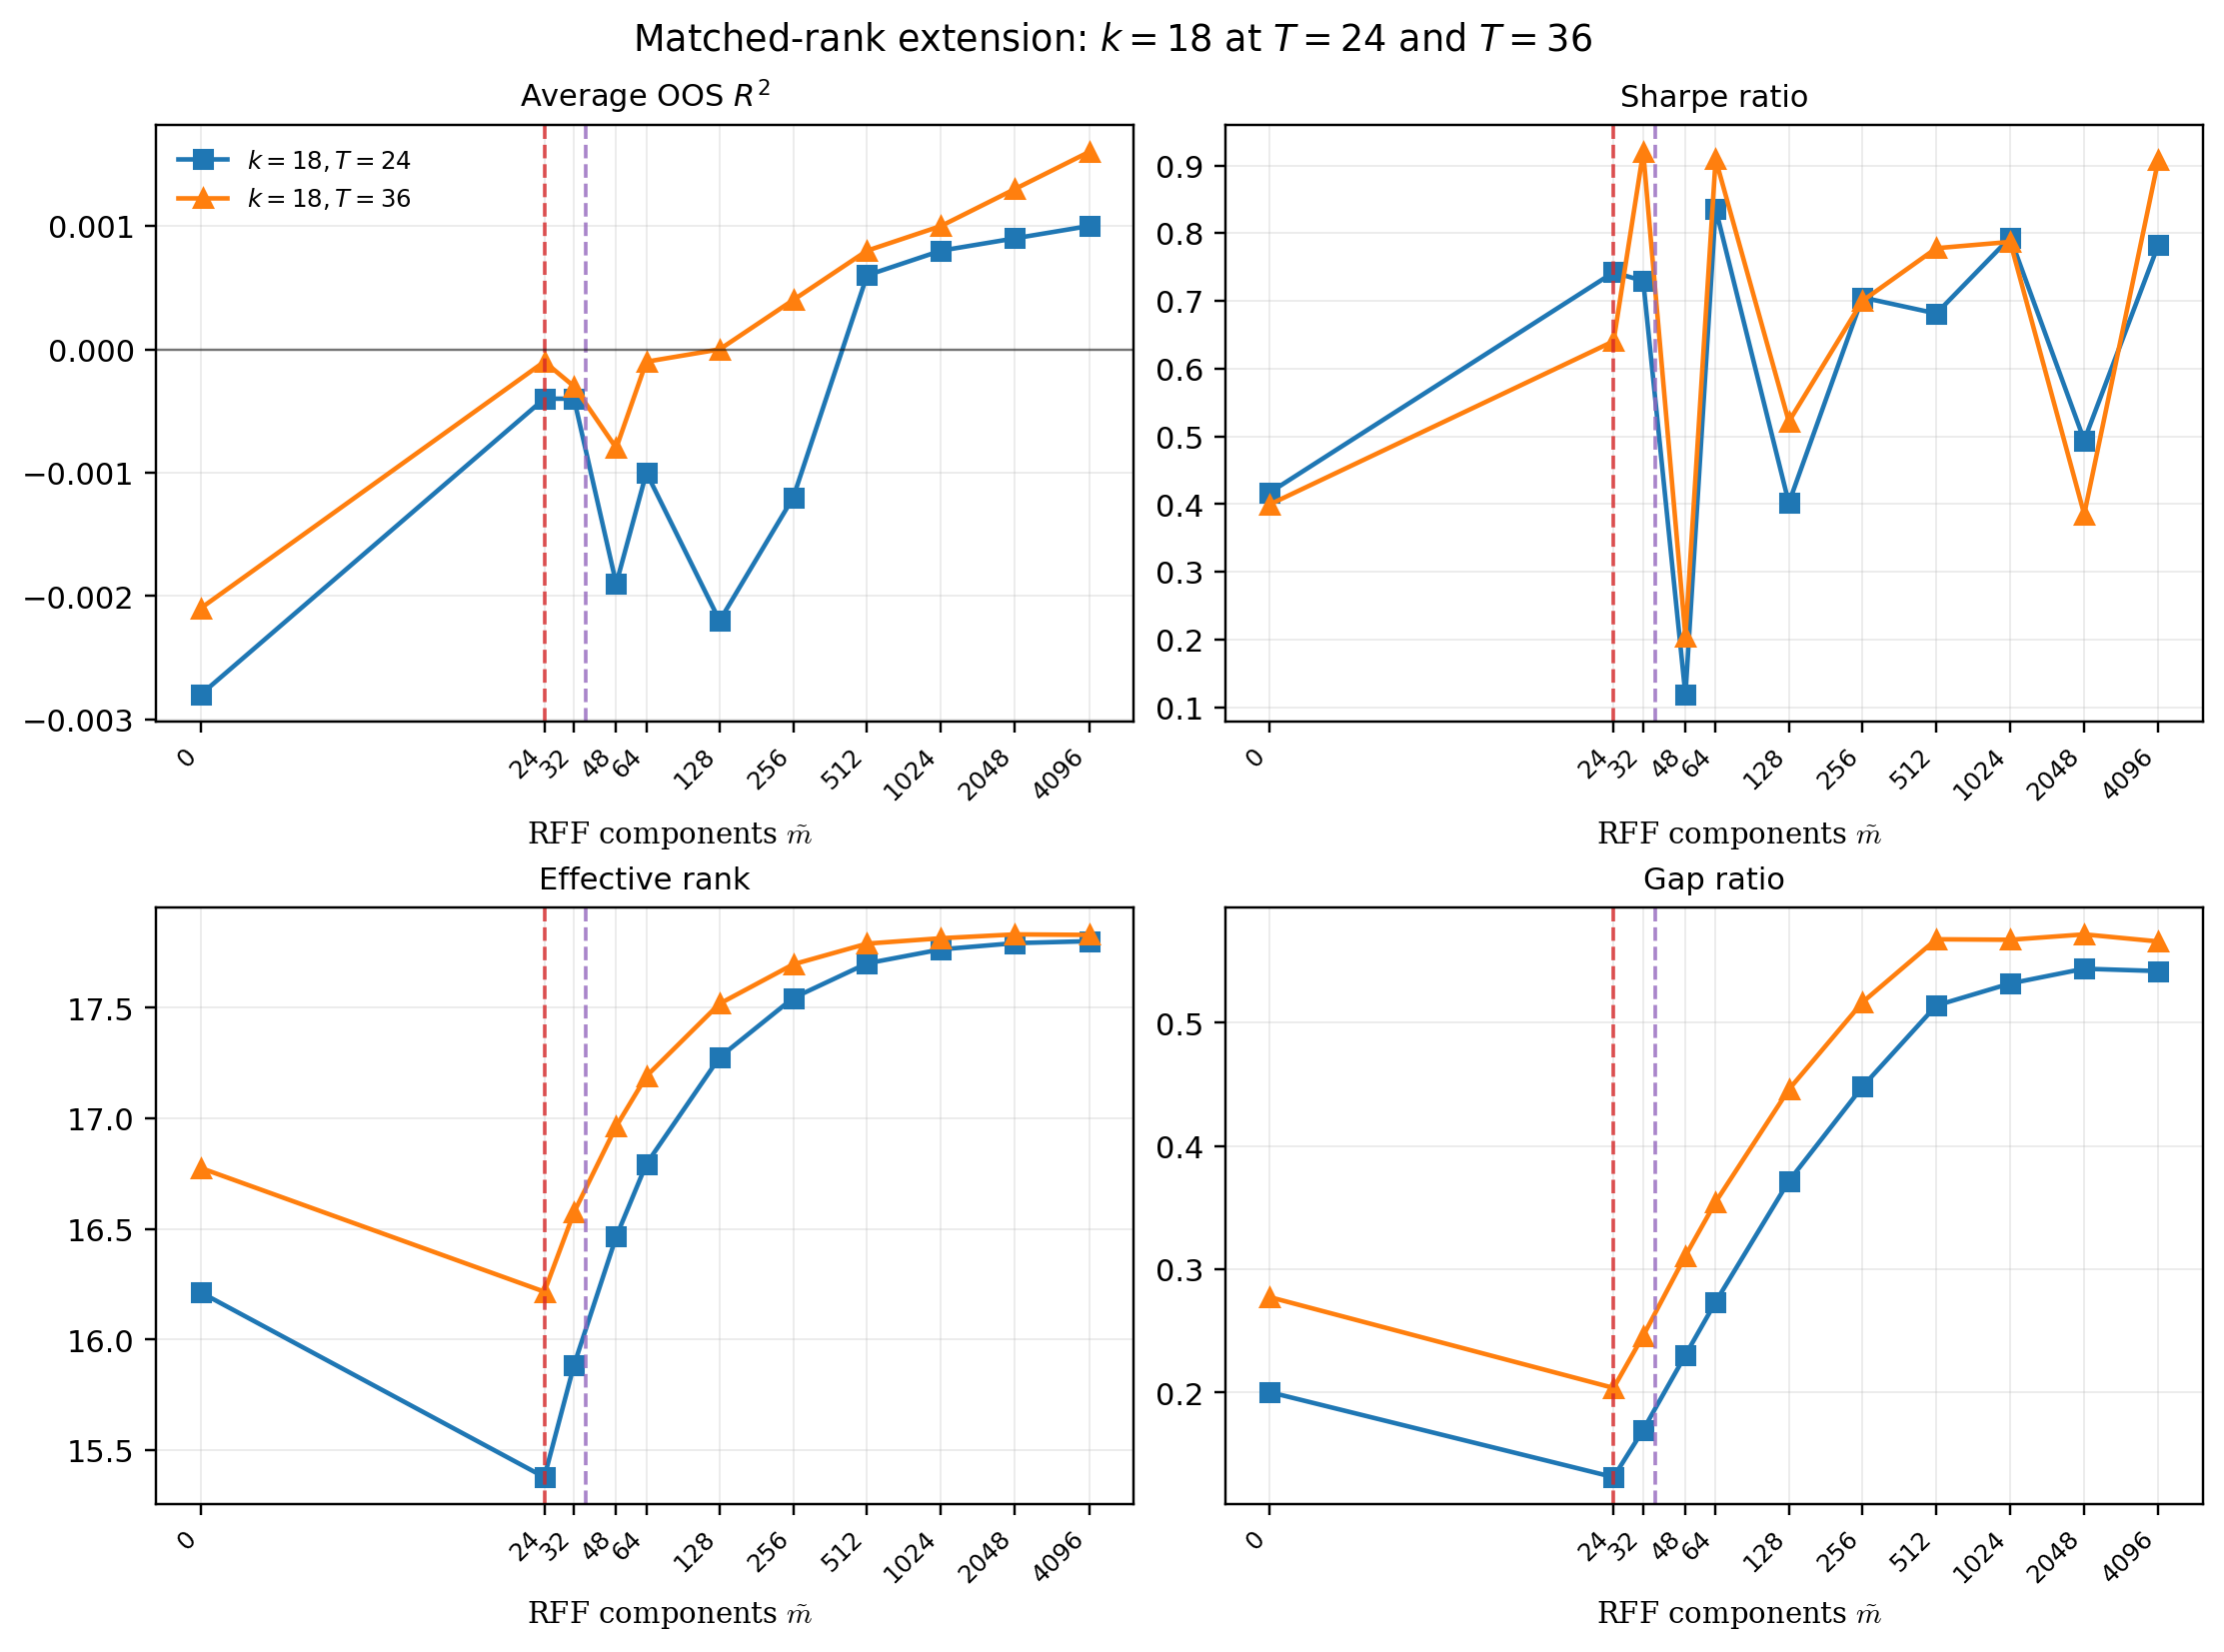
\includegraphics[width=0.97\linewidth]{synth_v5_window_compare.png}
\caption{Rank-aligned comparison across window lengths. The red dashed line marks $\tilde m/T=1$ at $\tilde m=24$ for $T=24$, and the purple dashed line marks $\tilde m/T=1$ at $\tilde m=36$ for $T=36$.}
\label{fig:sim:windowcompare}
\end{figure}

The new $T=36$ run is especially informative because it isolates the window-length effect without changing the fitted rank. Figure \ref{fig:sim:windowcompare} shows that the longer window raises the whole performance surface. The $T=36$ curve is less negative near the
boundary and more positive in the far-right tail, peaking at $0.0016$ rather than $0.0010$ in average out-of-sample $R^2$. The portfolio results improve in parallel: the baseline Sharpe is similar across windows, but the high-complexity region is stronger and smoother
at $T=36$, with especially strong values already around $\tilde m=32$ and $\tilde m=64$. The geometry is also cleaner. Effective rank pushes closer to $18$, and the gap ratio reaches a slightly higher plateau than at $T=24$.

\begin{figure}[H]
\centering
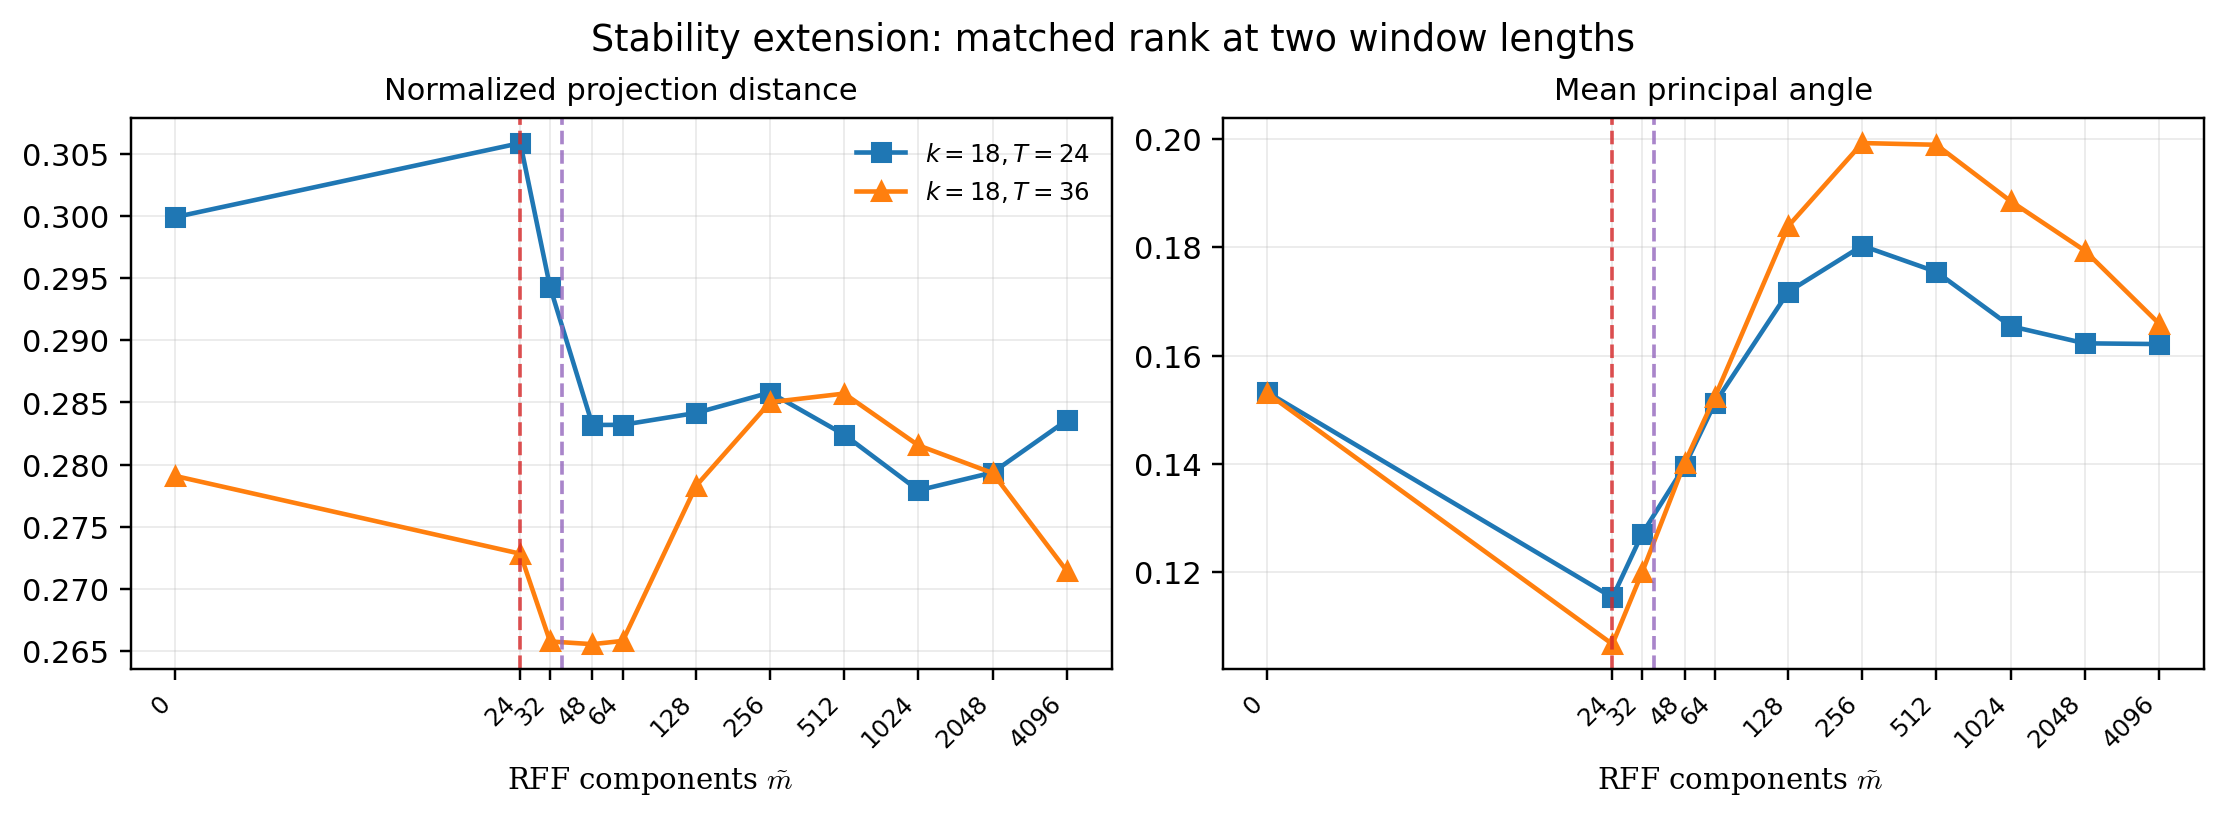
\includegraphics[width=0.97\linewidth]{synth_v5_window_stability.png}
\caption{Rank-aligned stability comparison across window lengths. The red dashed line marks $\tilde m/T=1$ at $\tilde m=24$ for $T=24$, and the purple dashed line marks $\tilde m/T=1$ at $\tilde m=36$ for $T=36$.}
\label{fig:sim:windowstability}
\end{figure}

Figure \ref{fig:sim:windowstability} shows that the better tail performance at $T=36$ does not come from simply tolerating much wilder subspace motion. Normalized projection distance stays broadly controlled as the lift grows, and the mean principal angle rises through the intermediate region and then eases back in the tail. In other words, the longer window strengthens the geometry--performance relation rather than overturning it.

This short-window extension therefore complements the broad-grid study in a natural way. The long-window synthetic exercise validates the structural diagnostics in a clean low-rank environment. The short-window extension then shows that when the estimation problem is made
much more data-scarce and the interpolation threshold becomes visible, richer feature lifts can still improve average out-of-sample fit, Sharpe, and intrinsic dimension, provided the fitted rank is not badly misaligned with the underlying synthetic rank.

\subsection{Synthetic Summary and Bridge to Asset pricing application}
\label{sec:sim:summary}

The synthetic experiments yield three types of conclusions: emergent validations of the geometric framework, theory-aligned structural checks, and one important absence that sharpens the interpretation of the historical results.

\medskip
\noindent\textit{Emergent validations.}
The strongest synthetic validations are those that are not mechanically built into the DGP. First, drift anisotropy is a powerful predictor of performance: low $\rho_\psi$ is associated with high Sharpe, even though the underlying Grassmann random walk is isotropic by construction. This makes the anisotropy result genuinely emergent and supports the interpretation of $\rho_\psi$ as a within-regime performance diagnostic. Second, the paired comparison between $z=0$ and $z>0$ reproduces the historical frozen-versus-regularized split without being calibrated to do so. The widening of that ratio with $k$ is precisely the pattern predicted by Theorem~\ref{thm:curv-erank}(i)--(ii). Third, in the short-window extension, rank-aligned specifications and moderately longer
training windows produce cleaner positive tails in average out-of-sample $R^2$, stronger Sharpe, and more favorable structural summaries. This does not follow mechanically from the DGP and should therefore be viewed as emergent finite-sample evidence.

\medskip
\noindent\textit{Theory-aligned structural checks.}
Other findings serve primarily as computational and structural validation of the framework. The sharp spectral-gap cliff at the true rank $k_0$ is exactly what Theorem~\ref{thm:curv-erank}(iii) predicts in the clean low-rank setting. Likewise, effective-rank collapse beyond $k_0$ confirms that additional nominal factors do not translate into additional intrinsic dimension once the signal space is exhausted. The monotone co-movement of the geometric metrics with regularization $z$ is also consistent with the curvature mechanism of Theorem \ref{thm:curv-erank}(ii): as regularization increases, the estimator moves away from flat directions and tracks the signal subspace more reliably. Finally, the erratic behavior at $z=0$ is the finite-sample manifestation of the same geometric degeneracy.

\medskip
\noindent\textit{Synthetic-historical contrast.}
One pattern that does \emph{not} appear in the clean synthetic DGP is the productive illusion reported in Section~\ref{sec:hist_data}: peak Sharpe does not occur just beyond the spectral cliff, but instead at the true signal rank. In the synthetic setting, there is no additional economic structure for overparameterization to exploit. The fact that this pattern is absent here but present in the baseline historical grid suggests that the historical phenomenon reflects genuine structure rather than a mechanical artifact of the estimator.

\medskip
\noindent\textit{Practical implications.}
The synthetic results validate three practical uses of the geometric diagnostics. First, \emph{grid narrowing}: spectral gap and $\dproj$ can eliminate clearly degenerate configurations before expensive out-of-sample evaluation. Second, \emph{within-regime ranking}: among surviving configurations, anisotropy $\rho_\psi$ separates focused from diffuse subspace motion, with lower values
structurally associated with stronger performance. Third, \emph{boundary monitoring}: in short-window problems, explicitly tracking where $\tilde m/T=1$ lies helps determine whether improvements occur near the interpolation threshold, in the overparameterized tail, or only because the fitted rank is misaligned with the underlying signal.

Overall, the synthetic exercise validates the geometric diagnostics in a controlled environment with known signal structure and clarifies which empirical patterns should be interpreted as structural rather than accidental. We now turn to historical US equity data, where the true factor structure is unknown, the characteristic space is richer, and structural breaks and nonlinearities are present. The central question is whether the same qualitative patterns---drift anisotropy as the strongest predictor, regime separation via $\dproj$, the
spectral-gap cliff at a finite $k_0$, and the Goldilocks zone in subspace stability---reappear in this more complex setting. Where synthetic and historical patterns agree, the geometric explanation is strengthened; where they diverge, the divergence itself is informative.


\section{Asset pricing application: RFF Model for US Equities}
\label{sec:hist_data}

We now apply the Grassmann--IPCA pipeline to historical US equity data. The purpose of this section is to test whether the geometric patterns isolated in the synthetic experiments reappear when the true factor structure is unknown, the characteristic space is richer, and structural breaks and nonlinearities are present.

The asset pricing application focuses on three empirical questions. First, does increasing the RFF feature dimension $\tilde m$ improve out-of-sample behavior, as predicted by the virtue-of-complexity mechanism? Second, do the geometric diagnostics identify the same structural regimes as in the synthetic study: frozen versus regularized behavior, spectral-gap cliffs, effective-rank saturation, and stable versus diffuse subspace motion? Third, does the historical data exhibit patterns that cannot arise in the clean linear DGP,
such as productive overparameterization beyond the apparent spectral boundary?

Across 88 backtest configurations of the Grassmann--IPCA model, spanning
factor dimensions $k$, RFF dimensions $\tilde m$, and ridge penalties $z$, we find
three robust patterns. First, Sharpe ratio and out-of-sample $R^2$ broadly
improve with feature dimension $\tilde m$ when $z>0$. Second, spectral gap and
effective rank act primarily as regime separators, identifying an empirical
signal dimension around $k_0\approx 16$--$20$, while drift anisotropy
$\rho_\psi=\bar\psi/\psi_{\max}$ acts as a within-regime performance
diagnostic. Third, the best historical Sharpe occurs just beyond the spectral
cliff, a phenomenon we interpret as a ridge-regularized productive illusion:
mild overparameterization appears to stabilize weak, persistent directions that
are absent from the clean synthetic DGP.

An extended backtest reported in Section~\ref{sec:extended} strengthens this
picture using a finer RFF grid, higher seed counts, and a longer training window
($T=36$). That specification produces the strongest results in the study, with
positive out-of-sample $R^2$ and Sharpe close to one in the high-complexity
region.

\subsection{Data, universe, and backtest protocol}
\label{sec:hist:setup}

The asset pricing experiments use a monthly equity panel where the baseline investable universe consists of the top
50 US equities by market capitalization over the full 1994--2025 history. This fixed-universe choice introduces a mild selection look-ahead when interpreting raw performance levels, since the identities of the large-cap stocks are chosen using the full sample. We accept this limitation here because the purpose of the baseline exercise is geometric: to study the fitted return subspaces and their diagnostics under a stable, computationally tractable universe, not to claim an implementable top-50 trading record. Section~\ref{sec:extended} returns to this point using rolling top-50 universes. For each
asset-month, the predictive information is encoded in a vector of 73 raw
characteristics. After preprocessing, these asset-level characteristics provide
the design matrix used in the Grassmann--IPCA estimation.

The baseline universe is intentionally moderate in size. Unlike the broad CRSP
cross-sections often used in empirical asset-pricing studies, where the number
of stocks can be in the thousands, the top-50 universe keeps the rolling
Riemannian optimization problem computationally tractable and makes the
resulting Grassmann diagnostics easier to interpret. This is especially
important because the historical experiments involve repeated optimization on
$\gr(k,\tilde m)$, with $\tilde m$ ranging up to $10{,}000$.

Before model fitting, characteristics are preprocessed cross-sectionally at
each month. Each characteristic is demeaned and scaled to unit cross-sectional
standard deviation. Missing values are imputed with cross-sectional means, and
assets with more than $30\%$ missing observations or zero returns are removed
from the panel. The resulting asset-month vectors
$x_{i,t}\in\bR^{73}$ are used in both the linear and RFF-lifted
specifications.

For each rolling estimation window, we fit a Grassmann--IPCA model with an RFF
lift of the asset-level characteristic vector and ridge regularization. The
baseline historical grid contains 88 configurations across
\begin{equation*}
	k \in \{4,8,12,16,20,24,28,32\},
	\qquad
	\tilde m \in \{64,\ldots,10{,}000\},
	\qquad
	z \in \{0,\ldots,100\}.
\end{equation*}
Here $k$ is the nominal factor dimension, $\tilde m$ is the RFF feature dimension,
and $z$ is the ridge penalty. Unless otherwise stated, the rolling training
window has length $T=24$ months. The model is estimated by warm-started
Riemannian conjugate-gradient optimization on the relevant Grassmann manifold.

At each out-of-sample month, portfolio weights are proportional to the
predicted cross-sectional returns and are rescaled by the mean absolute
prediction,
\begin{equation*}
w_{i,t}
=
\frac{\hat r_{i,t}}
{N_t^{-1}\sum_{j=1}^{N_t}|\hat r_{j,t}|+10^{-12}} .
\end{equation*}
The portfolio return is then
\begin{equation*}
r_t^{\mathrm{port}}
=
\frac{1}{N_t}\sum_{i=1}^{N_t} w_{i,t} r_{i,t+1}.
\end{equation*}
Sharpe ratios are annualized using the monthly-data factor $\sqrt{12}$, and
all reported Sharpe ratios are gross of transaction costs.

The purpose of this design is diagnostic rather than production-oriented. The
asset pricing experiment asks whether the geometric mechanisms observed in the
synthetic study; spectral-gap effects, anisotropy-performance relationships,
effective-rank behavior, and the emergence of a Goldilocks complexity
region; also appear in a real monthly equity panel. The small-universe design should therefore be
read as a controlled empirical test of the geometry, rather than as a claim
about full-market implementation.

\subsection{RFF feature lift the asset pricing experiment}
\label{sec:hist:rff}

Section~\ref{sec:rff} introduced the random Fourier feature construction in
general terms. Here we specify how that construction is used in the asset pricing  experiment.

Let $x_{i,t}\in \bR^d$ denote the preprocessed characteristic vector for asset $i$ at month $t$,
with $d=73$ before any nonlinear expansion. The preprocessing includes the
same winsorization, standardization, and missing-value treatment used in the
baseline linear specification. The linear benchmark uses $x_{i,t}$ directly.
The nonlinear specifications replace $x_{i,t}$ by its RFF lift $\phi_{\tilde m}(x_{i,t})\in \bR^{\tilde m}$,
using the Gaussian-kernel convention described in Section~\ref{sec:rff}. Thus $\tilde m$ controls the dimension of the randomized
nonlinear dictionary generated from the original asset-level characteristics.

At each date $t$, the original characteristic matrix
\begin{equation*}
	Z_t =
	\begin{pmatrix}
		x_{1,t}^{\top}\\
		\vdots\\
		x_{N_t,t}^{\top}
	\end{pmatrix}
	\in \mathrm{Mat}_{N_t,d}(\bR)
\end{equation*}
is replaced by the lifted matrix
\begin{equation*}
	\Phi_t^{(\tilde m)}
	=
	\begin{pmatrix}
		\phi_{\tilde m}(x_{1,t})^{\top}\\
		\vdots\\
		\phi_{\tilde m}(x_{N_t,t})^{\top}
	\end{pmatrix}
	\in \mathrm{Mat}_{N_t,\tilde m}(\bR).
\end{equation*}
Unless otherwise stated, the RFF bandwidth is fixed at $\gamma=0.25$, and
different RFF seeds correspond to independent draws of the random frequencies
and phases.

The subsequent IPCA estimation step is unchanged. For a nominal factor
dimension $k$, the rolling-window model is
\begin{equation*}
	r_{t+1}
	=
	\Phi_t^{(\tilde m)}\Gamma^\top f_{t+1}
	+
	\varepsilon_{t+1},
	\qquad
	\Gamma\in \mathbb{R}^{k\times \tilde m},
	\qquad
	f_{t+1}\in \mathrm{Mat}_{k,\tilde m}(\bR).
\end{equation*}
Equivalently, the asset loadings are
\begin{equation*}
	\beta_t
	=
	\Phi_t^{(\tilde m)}\Gamma^\top .
\end{equation*}
The estimated geometric object in each rolling window is therefore
\begin{equation*}
	\operatorname{row}(\Gamma)\in \gr(k,\tilde m),
\end{equation*}
the $k$-dimensional subspace of the $\tilde m$-dimensional RFF characteristic
space selected by the IPCA estimator.

This formulation makes clear that the RFF lift is
applied asset by asset to the characteristic vector associated with each
asset-month observation. Increasing $\tilde m$ therefore enriches the nonlinear
characteristic dictionary available to the estimator, while $k$ continues to
fix the dimension of the fitted return-producing subspace. The rolling-window
protocol, ridge penalty, portfolio-construction rule, and out-of-sample
evaluation are otherwise identical across the linear and nonlinear
specifications.

\subsection{Diagnostic taxonomy}
\label{sec:hist:taxonomy}

We use the same geometric diagnostics as in the synthetic section:
\begin{equation*}
	\dproj,\qquad
	\psi_{\max},\qquad
	\bar\psi,\qquad
	\rho_\psi=\frac{\bar\psi}{\psi_{\max}},
	\qquad
	\erank(\hat{\Sigma}_f),
	\qquad
	\mathrm{sg}.
\end{equation*}
Here $\dproj$ denotes the normalized projection distance between estimated
subspaces, $\psi_{\max}$ and $\bar\psi$ summarize the principal-angle
spectrum, $\rho_\psi$ measures the anisotropy of subspace drift,
$\erank(\hat{\Sigma}_f)$ is the effective rank of the estimated factor
covariance matrix, and $\mathrm{sg}$ denotes the relevant spectral-gap
diagnostic.

These diagnostics play two distinct empirical roles.

\emph{Regime separators} identify where a configuration lies in the geometry of
the estimation problem. The spectral gap and effective rank are the main
examples. They indicate whether the fitted dimension is below, near, or beyond
the empirical signal boundary. Projection distance and principal-angle
magnitudes also contribute to this classification by measuring how rapidly the
estimated subspace changes across rolling windows. These quantities should not,
however, be interpreted as performance rankings by themselves.

\emph{Sharpe supporters} diagnose whether the observed subspace motion is likely
to be economically useful. Drift anisotropy $\rho_\psi$ is the leading
example. A low value of $\rho_\psi$ means that subspace adjustment is
concentrated in a few principal directions rather than spread diffusely across
many weakly identified directions. In the historical experiments, this
distinction is important because two configurations can have similar overall
subspace movement but very different principal-angle spectra, and hence very
different implications for out-of-sample portfolio performance.

\subsection{Regime separation via \texorpdfstring{$d_{\mathrm{proj}}$}{d\_proj}}
\label{sec:regime}

The first historical diagnostic asks whether the rolling estimator is genuinely
moving through the Grassmannian, or whether it is effectively frozen near its
warm start. This distinction is visible from training-window objects alone. For
each configuration, we compute the projection distance between the warm-started
initial subspace and the optimized subspace. To make values comparable across
different choices of $k$ and $\tilde m$, we report the Haar-normalized distance
\begin{equation*}
	\widetilde d_{\mathrm{proj}}
	=
	\frac{d_{\mathrm{proj}}}{b_{\tilde m,k}},
	\qquad
	b_{\tilde m,k}
	=
	\left(\frac{2k(\tilde m-k)}{\tilde m+1}\right)^{1/2},
\end{equation*}
where $b_{\tilde m,k}$ is the expected projection distance between two independent
Haar-random $k$-planes in $\mathbb{R}^{\tilde m}$. Values close to zero indicate a
geometrically frozen configuration, while values closer to one indicate movement
on the scale of a typical random displacement in $\gr(k,\tilde m)$.

Figure~\ref{fig:regime} shows that the unregularized and regularized
configurations occupy sharply different geometric regimes. The unregularized
specifications with $z=0$ cluster at very low normalized projection distance,
whereas regularized specifications with $z>0$ exhibit substantially larger
movement away from the warm start.

\begin{figure}[H]
	\centering
	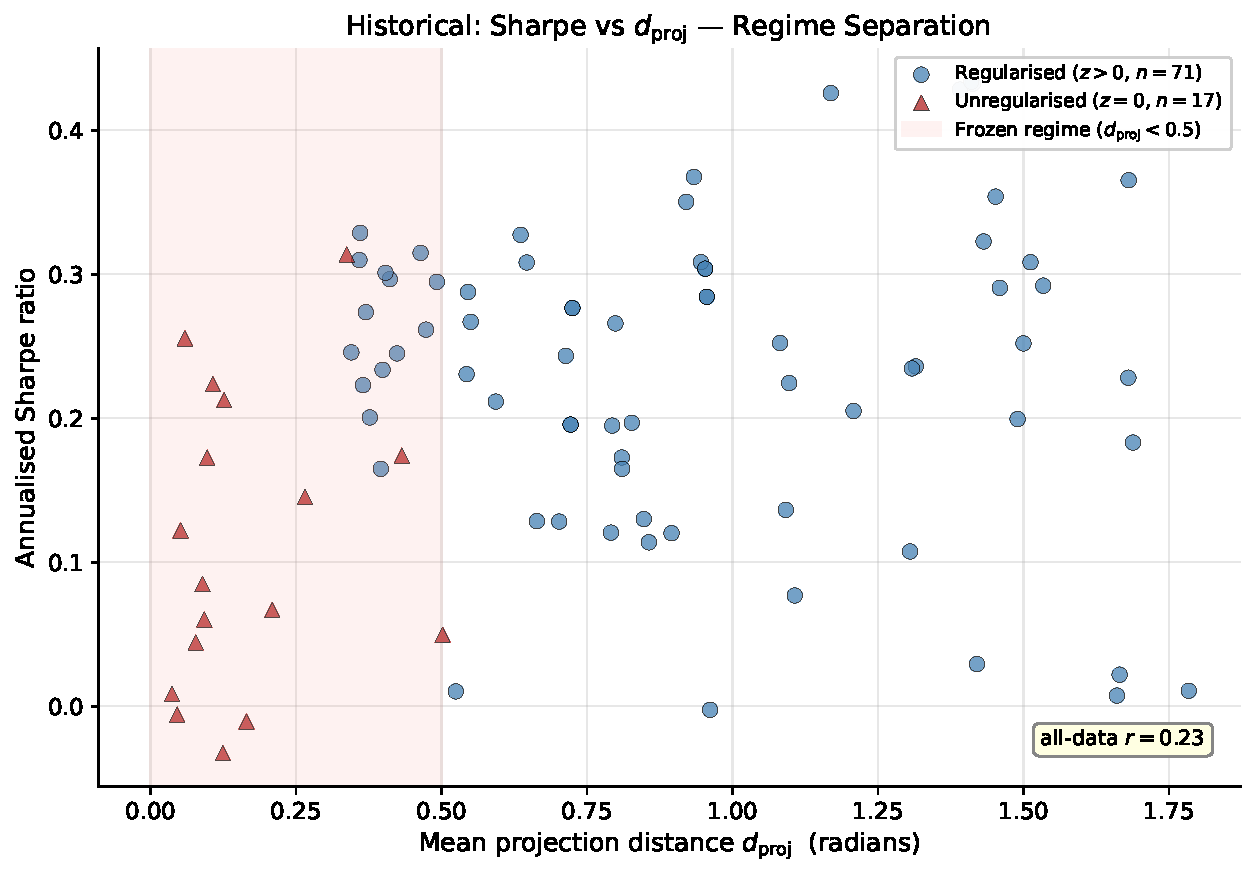
\includegraphics[width=0.78\textwidth]{fig1_regime.pdf}
	\caption{Annualized Sharpe ratio versus the mean warm-started
		projection distance $d_{\mathrm{proj}}$ across the historical
		configurations in our dataset. The shaded vertical region marks
		the frozen regime; unregularized configurations ($z=0$, red
		triangles) cluster there, indicating warm-start solutions that
		barely move on the Grassmannian. Regularized configurations
		($z>0$, blue circles) move substantially farther from the warm
		start and occupy the active estimation regime. The all-data
		Pearson correlation between $d_{\mathrm{proj}}$ and Sharpe is
		reported in the inset.}
	\label{fig:regime}
\end{figure}

The separation is also visible in the summary statistics:
\begin{table}[H]
	\centering
	\small
	\begin{tabular}{lccc}
		\toprule
		& \textcolor{illred}{\textbf{Unregularized} ($z=0$)}
		& \textcolor{virtblue}{\textbf{Regularized} ($z>0$)}
		& Ratio \\
		\midrule
		$n$
		& 17
		& 71
		& --- \\
		Mean Sharpe
		& $0.111 \pm 0.102$
		& $0.233 \pm 0.104$
		& $2.10\times$ \\
		Mean $\widetilde d_{\mathrm{proj}}$
		& $0.166$
		& $0.937$
		& $\mathbf{5.65\times}$ \\
		\bottomrule
	\end{tabular}
	\caption{Regime summary statistics across the 88 historical configurations.
		The reported distance is Haar-normalized, so values near zero correspond to
		frozen configurations and values near one correspond to movement on the
		scale of a typical random displacement in $\gr(k,\tilde m)$.}
	\label{tab:regime-summary}
\end{table}

This empirical separation is consistent with the curvature mechanism developed
in Theorem~\ref{thm:curv-erank}. When $k>k_0$, the Riemannian Hessian contains
a null space of dimension $(k-k_0)(\tilde m-k_0)$. In the unregularized case, the
effective eigenvalue gaps are small, leaving many weak directions with little
curvature. The warm-started optimizer can therefore remain close to its initial
subspace, producing very small $\widetilde d_{\mathrm{proj}}$. Ridge
regularization increases curvature in these weak directions through the
ridge--curvature channel, allowing the estimator to move into an active
Grassmannian regime.

For example, at $k=32$ and $z=0$, the normalized distance is only
\begin{equation*}
\widetilde d_{\mathrm{proj}} = 0.092.
\end{equation*}
Since the corresponding Haar baseline is
\begin{equation*}
b_{\tilde m,k}
=
\left(\frac{2k(\tilde m-k)}{\tilde m+1}\right)^{1/2}
\approx 7.98,
\end{equation*}
this means that the actual displacement is only about $9.2\%$ of a typical
random Grassmannian displacement. The configuration is therefore not merely
low-performing; it is geometrically frozen.

\subsection{\texorpdfstring{Ridge regularization and Grassmannian motion}{Ridge regularization and Grassmannian motion}}
\label{sec:zsweep}

The previous subsection showed that the unregularized specifications tend to be
geometrically frozen. We next examine a single controlled ridge sweep, holding
$k=12$ and $\tilde m=1024$ fixed while varying the ridge penalty $z$. This
isolates the effect of regularization on the motion of the fitted subspace.

Figure~\ref{fig:zsweep} reports the projection distance, maximum principal
angle, mean principal angle, and out-of-sample Sharpe ratio along this ridge
path. In this slice of the historical grid, the geometric diagnostics and the
Sharpe ratio move together: increasing $z$ moves the optimizer farther away
from its warm start, increases the principal-angle magnitudes, and improves
out-of-sample performance.

In the implementation, the ridge parameter $z$ enters through the profiled
factor-estimation step. For a fixed subspace representative $W$, let
\begin{equation*}
\Lambda_t = Z_t W .
\end{equation*}
The factor estimate is computed from the regularized normal equations
\begin{equation*}
\hat f_t
=
(\Lambda_t^\top \Lambda_t + z I_k)^{-1}
\Lambda_t^\top r_t .
\end{equation*}
Thus $z$ stabilizes the weak directions in the profiled least-squares problem.
This is the computational channel through which ridge regularization changes
the local conditioning and curvature of the Grassmannian objective.

\begin{figure}[H]
	\centering
	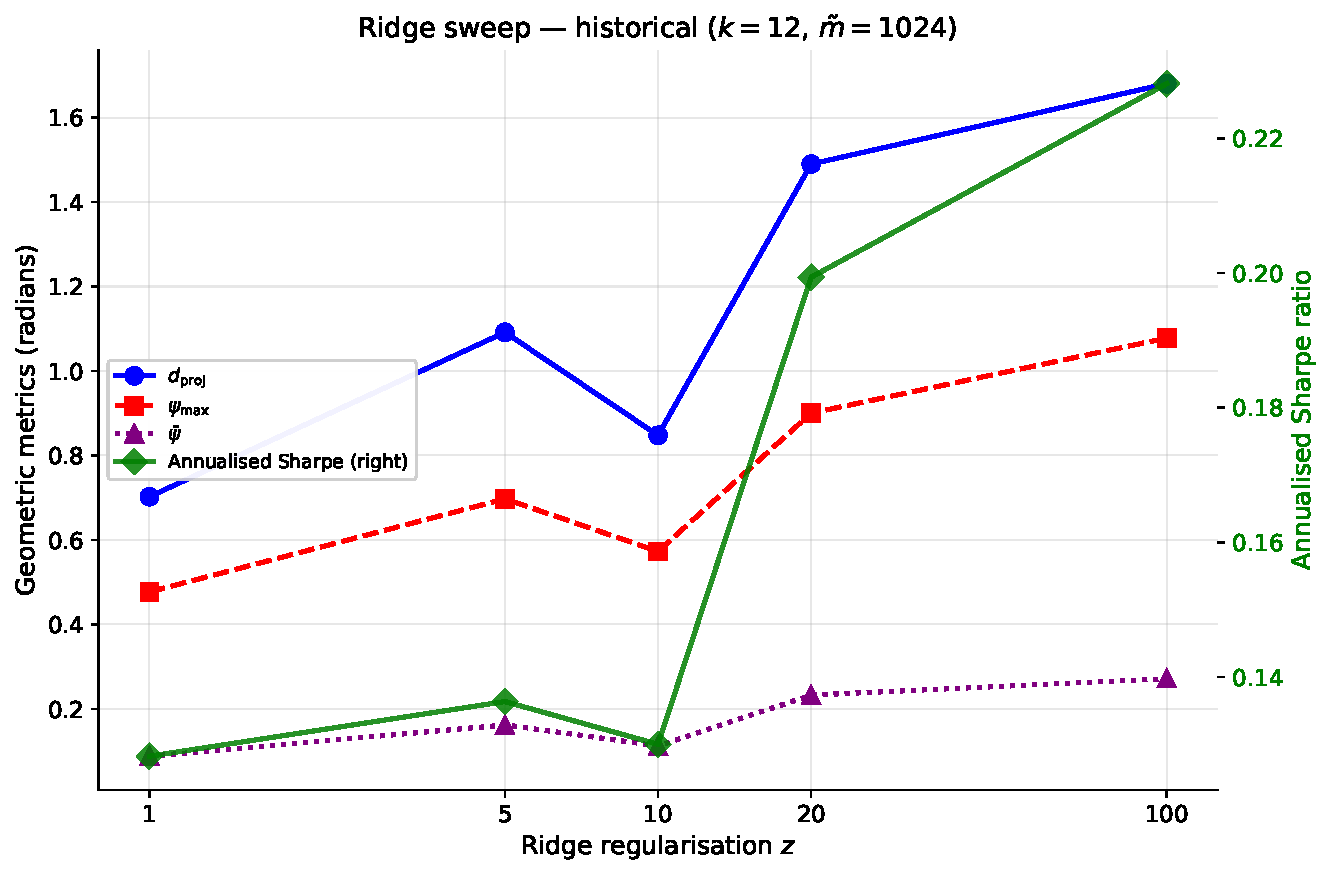
\includegraphics[width=0.78\textwidth]{fig3_zsweep.pdf}
	\caption{Ridge sweep for the asset pricing experiment at
		$k=12$ and $\tilde m=1024$. The left axis reports the Grassmannian
		diagnostics $d_{\mathrm{proj}}$, $\psi_{\max}$, and $\bar\psi$
		in radians; the right axis reports the out-of-sample annualized
		Sharpe ratio. Along this controlled path, increasing the ridge
		penalty moves the fitted subspace farther from its warm start and
		is associated with higher Sharpe. (Values at $z=20$ are averaged
		over the two rolling-window sub-runs that visit this point.)}
	\label{fig:zsweep}
\end{figure}

Over the range $z=1$ to $z=100$, the Sharpe ratio increases by approximately
$0.100$, the projection-distance diagnostic increases by approximately
$0.978$, and the maximum principal angle increases by approximately
$0.60$ radians. The important point is not that ridge mechanically improves
every configuration, but that in this representative slice it unlocks
Grassmannian motion that is suppressed in the nearly unregularized regime.

This behavior is consistent with the curvature mechanism of
Theorem~\ref{thm:curv-erank}. When the fitted dimension exceeds the effective
signal dimension, many directions are weakly identified. Ridge regularization
improves the conditioning of these weak directions, increases the effective
curvature of the local objective, and allows the warm-started optimizer to move
toward a more informative subspace. The historical ridge sweep therefore gives
a concrete empirical instance of the ridge--curvature channel developed above.


\subsection{\texorpdfstring{The spectral-gap cliff and the empirical signal boundary}{The spectral-gap cliff and the empirical signal boundary}}
\label{sec:specgap}

The next diagnostic asks where the empirical signal boundary lies as the fitted
factor dimension $k$ increases. For this purpose, we examine the spectral-gap
diagnostic $\mathrm{sg}$ computed from the estimated factor covariance. The
basic interpretation is the same as in the synthetic analysis: when the fitted
dimension remains within the signal-bearing range, the gap stays meaningfully
positive; once $k$ moves beyond the effective signal dimension, the trailing
factors approach the noise floor and the gap collapses toward zero.

Figure~\ref{fig:specgap} plots the spectral-gap diagnostic as a function of
$k$ at $\tilde m=1024$, for several values of the ridge penalty. The regularized
curves are the most informative, since the unregularized specifications are
partly affected by the frozen-regime phenomenon discussed above. For
$z=10$ and $z=20$, the gap remains visibly positive at $k=16$ and falls
to near zero by $k=20$. This places the empirical signal boundary in the
historical experiment at approximately $k=16$--$20$.

\begin{figure}[H]
	\centering
	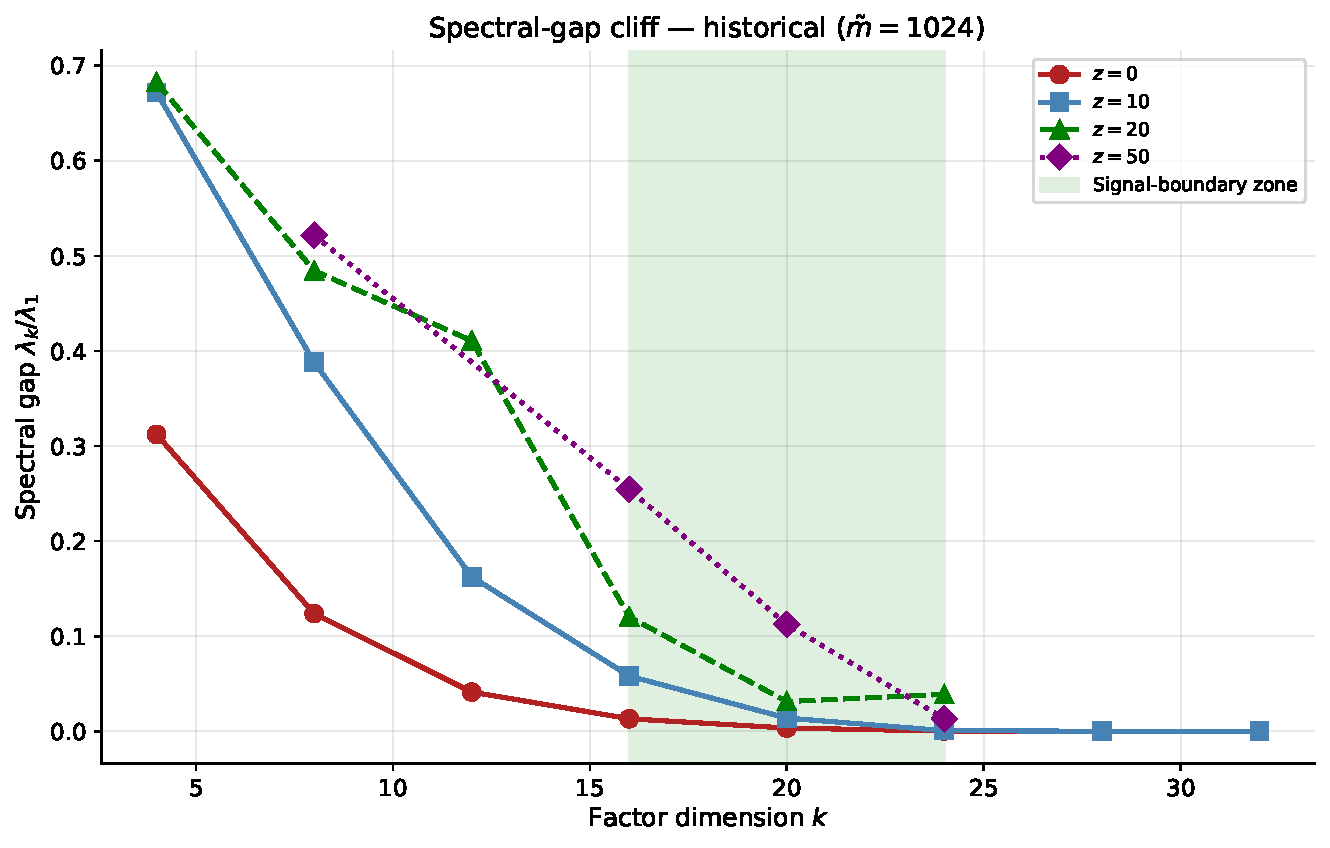
\includegraphics[width=0.78\textwidth]{fig7_specgap.pdf}
	\caption{Spectral-gap diagnostic $\lambda_k/\lambda_1$ versus factor
		dimension $k$ at $\tilde m=1024$, for two regularized values of $z$.
		The shaded vertical band marks the empirical signal boundary
		$k_0\approx 16$--$20$, where the gap collapses to near zero. The
		highest-Sharpe configurations (Table~\ref{tab:specgap-summary})
		occur slightly beyond this boundary rather than deep inside the
		strongly identified regime.}
	\label{fig:specgap}
\end{figure}

This is already informative by itself: the spectral-gap cliff separates a
clearly identified regime from a weak-gap regime in which additional fitted
directions lie near the empirical noise floor. More interestingly, however, the
best Sharpe ratios in the historical grid do not occur well inside the
identified regime. Instead, they occur slightly beyond the cliff, typically at
$k=20$--$24$, where the spectral gap has already collapsed.

\begin{table}[H]
	\centering\small
	\begin{tabular}{lccc}
		\toprule
		Config & Sharpe & $\mathrm{sg}$ & Regime \\
		\midrule
		$k=12, \tilde m=4096, z=50$  & 0.368 & 0.209 & Inside the boundary ($k<16$) \\
		$k=20, \tilde m=4096, z=50$  & 0.428 & 0.000 & At the upper edge of the boundary band \\
		$k=24, \tilde m=4096, z=100$ & 0.434 & 0.000 & Past the boundary \\
		$k=32, \tilde m=6000, z=20$  & 0.231 & 0.000 & Deep beyond the boundary \\
		\bottomrule
	\end{tabular}
	\caption{Representative historical configurations across spectral-gap
		regimes, where the empirical signal boundary $k_0\approx 16$--$20$
		corresponds to the shaded band in Figure~\ref{fig:specgap}. The
		spectral-gap diagnostic correctly locates the structural transition,
		while the best-performing configurations occur slightly beyond the
		boundary rather than well inside it.}
	\label{tab:specgap-summary}
\end{table}

This pattern is one of the more distinctive empirical findings of the
historical analysis. In the synthetic study, the cliff mainly acts as a regime
boundary. In the historical experiment, by contrast, the most successful
configurations lie just beyond that boundary. A natural interpretation is that
once $k$ moves slightly above the effective signal dimension, the model gains
additional flexibility in the representation of the return-producing subspace,
while ridge regularization keeps the extra weak directions from becoming
destabilizing.

This interpretation is consistent with the geometric diagnostics developed
earlier. The spectral gap indicates that the trailing fitted directions are no
longer strongly identified in the covariance spectrum, but the anisotropy
evidence shows that the resulting subspace motion is still highly concentrated.
At the best-performing configurations, $\psi_{\max}$ is substantial while
$\bar\psi$ remains small, indicating that only a small number of directions
are actively evolving. In other words, the model appears to benefit from
operating just beyond the spectral boundary, provided that ridge
regularization is strong enough to stabilize the extra directions.


\subsection{Drift anisotropy in the historical experiment}
\label{sec:hist:aniso}

Having located the empirical signal boundary via the spectral-gap diagnostic,
we now turn to the within-regime question: among configurations that lie in
the active estimation regime, which deliver the highest Sharpe? The synthetic
experiments identified drift anisotropy
$\rho_\psi = \bar\psi/\psi_{\max}$ as the strongest single predictor of
performance (Section~\ref{sec:sim:aniso}). Figure~\ref{fig:hist:aniso} shows
that the same pattern holds in the historical data, though with a somewhat
attenuated effect size, consistent with the noisier empirical environment.

\begin{figure}[H]
	\centering
	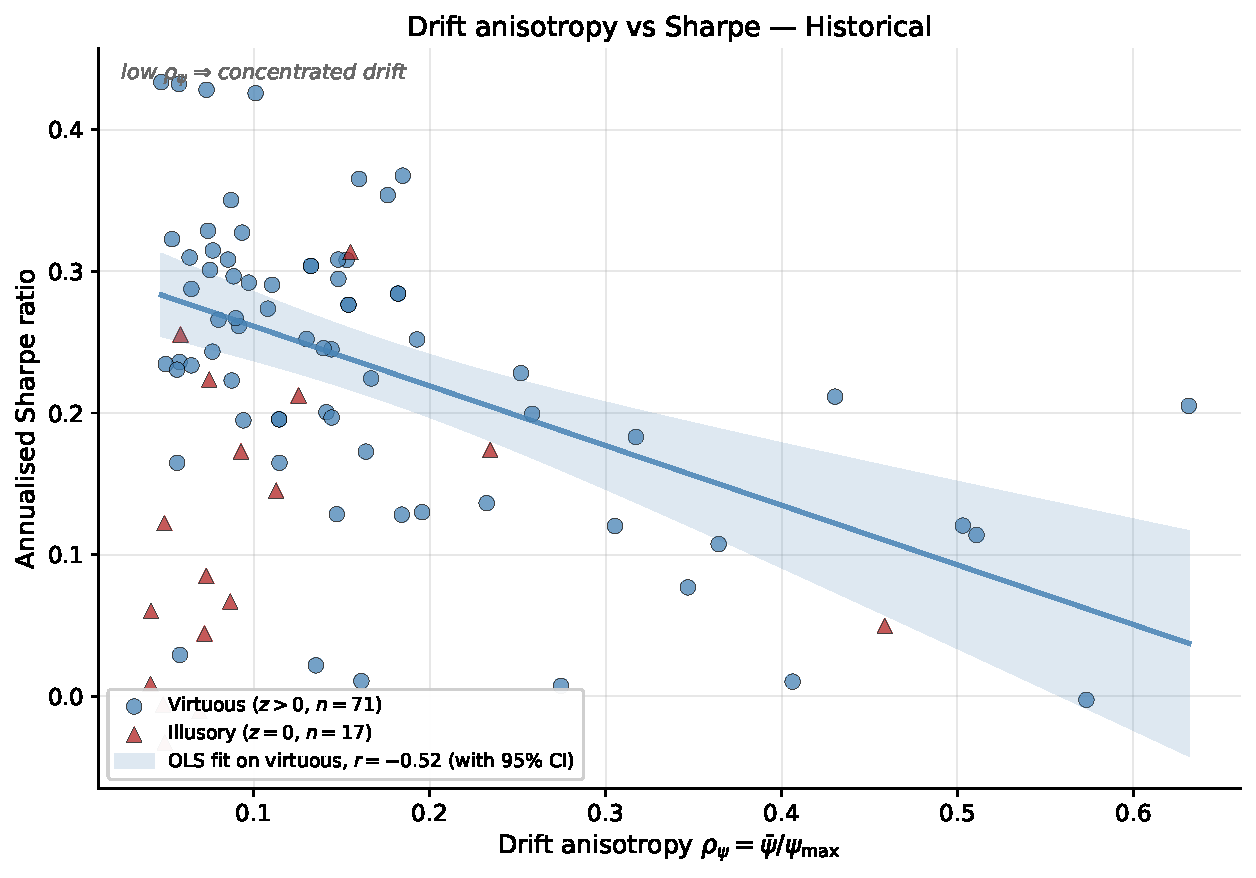
\includegraphics[width=0.78\textwidth]{fig_hist_aniso.pdf}
	\caption{Drift anisotropy
		$\rho_\psi = \bar\psi/\psi_{\max}$ versus annualized Sharpe ratio
		across the 88 historical configurations. Each marker is one
		$(k,z,\tilde m)$ configuration: blue circles are the regularized
		regime ($z>0$, virtuous, $n=71$), red triangles are the unregularized
		regime ($z=0$, illusory, $n=17$). The solid line is an OLS fit to the
		virtuous configurations and the shaded band is its 95\% confidence
		interval. The fitted within-regime correlation is $r=-0.52$, matching
		the value reported in Table~\ref{tab:sim:corr}; the all-data
		correlation is $r=-0.29$.}
	\label{fig:hist:aniso}
\end{figure}

The qualitative picture is the same as in the synthetic study: low anisotropy
(subspace motion concentrated in a small number of leading principal
directions) is associated with higher Sharpe, while high anisotropy (motion
spread broadly across many directions) is associated with weaker performance.
The within-virtuous-regime correlation, $r=-0.52$, is weaker than the
synthetic value of $-0.77$ but is the strongest single cross-sectional
diagnostic in the historical data. The illusory configurations cluster in a
narrow range of low $\rho_\psi$ at low Sharpe, reflecting the frozen
character of unregularized solutions discussed in Section~\ref{sec:regime}.
Together, these patterns confirm that anisotropy is informative
\emph{within} the active regime, rather than as a regime separator.

\subsection{Sharpe versus subspace stability: the Goldilocks zone}
\label{sec:goldilocks}

The previous diagnostics separate frozen configurations from active ones and
identify the spectral boundary in factor dimension. We now combine these ideas
by asking whether there is an empirically preferred range of subspace movement.
The answer is yes: the highest-Sharpe configurations are neither frozen nor
excessively unstable, but lie in an intermediate region of Grassmannian motion.

Figure~\ref{fig:goldilocks} plots Sharpe against the Haar-normalized projection
distance across all 88 historical configurations. Very small values of
$d_{\mathrm{proj}}$ correspond to the frozen regime discussed above: the
optimizer remains close to its warm start and fails to adapt meaningfully to the
training window. At the other extreme, very large values indicate substantial
subspace movement, which need not be economically useful unless it is
concentrated in stable signal directions. In this baseline top-50, $T=24$ grid, the best configurations concentrate
in an intermediate range,
\begin{equation*}
d_{\mathrm{proj}} \in [0.3,1.0],
\end{equation*}
with the top-performing specifications lying near the upper boundary of this
case-specific region. We do not interpret these numbers as universal cutoffs; they are the empirical range for this dataset, universe, and backtest design.

\begin{figure}[H]
	\centering
	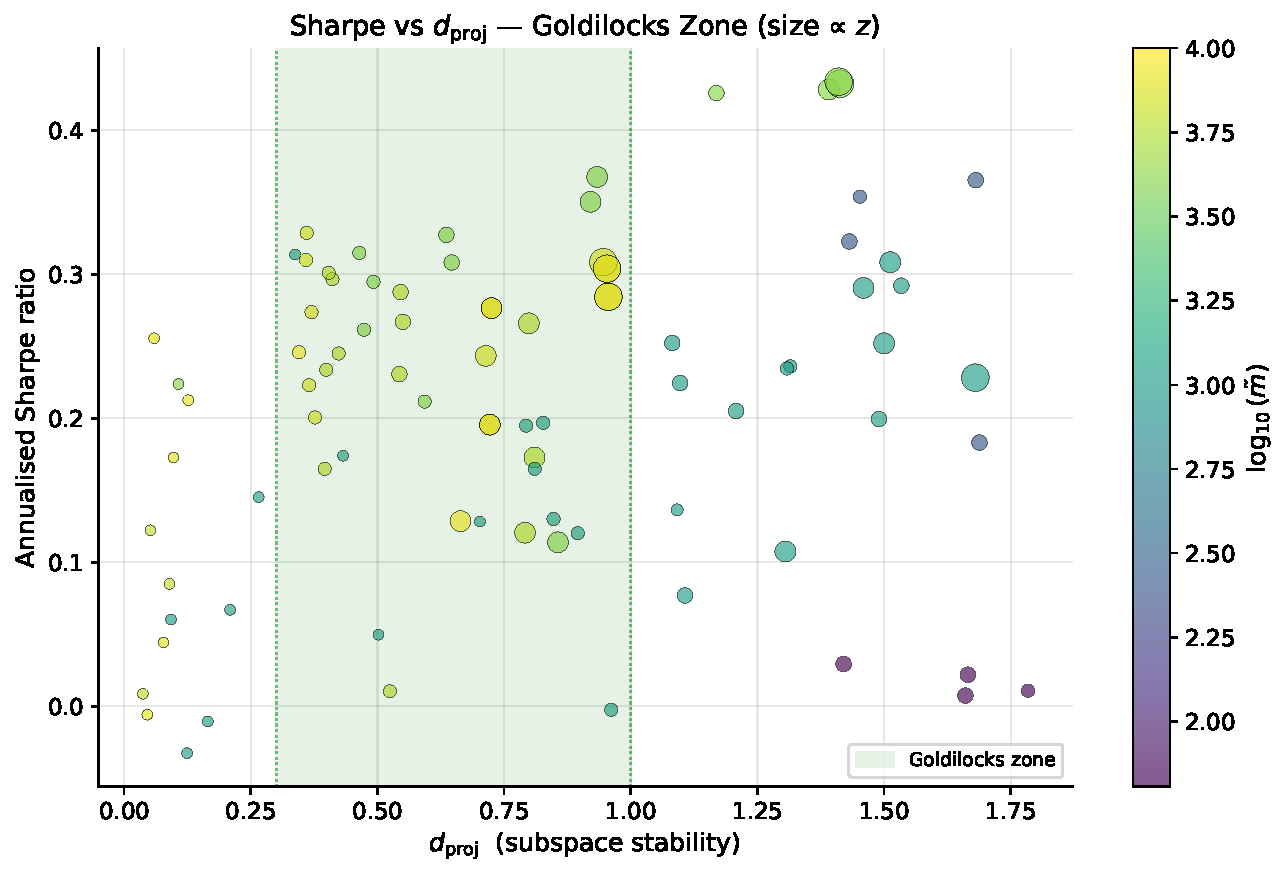
\includegraphics[width=0.78\textwidth]{fig_goldilocks.pdf}
	\caption{Annualized Sharpe ratio versus the mean warm-started
		projection distance $d_{\mathrm{proj}}$ across the historical
		configurations. Marker color encodes $\log_{10}(\tilde m)$ and marker
		size is proportional to the ridge penalty $z$. The shaded band
		marks the empirical Goldilocks zone
		$d_{\mathrm{proj}}\in[0.3,1.0]$ for this baseline grid, where the
		highest-Sharpe configurations concentrate; these dominate both the
		low-distance ``frozen'' configurations to its left and the
		high-movement ``wandering'' configurations to its right.}
	\label{fig:goldilocks}
\end{figure}

This intermediate region is the empirical Goldilocks zone for the baseline grid. It corresponds to
configurations in which the estimated subspace moves enough to incorporate new
information, but not so much that the motion becomes diffuse or unstable. The
interpretation is consistent with the anisotropy evidence: the most successful
models are not those with maximal subspace movement, but those whose movement is
both substantial and concentrated in a small number of principal directions.


\subsection{Asset pricing results synthesis}
\label{sec:hist:summary}

Taken together, the historical evidence supports the main geometric distinction developed earlier in the paper. Some diagnostics act primarily as \emph{regime separators}: spectral-gap collapse, effective-rank behavior, and the concentration of unregularized configurations in the frozen regime identify where the fitted model has moved beyond the well-identified signal subspace described by Theorem~\ref{thm:curv-erank}. Other diagnostics are more informative \emph{within} the active regime: low anisotropy $\rho_\psi=\bar\psi/\psi_{\max}$, moderate $d_{\mathrm{proj}}$, and the regularized increase in Grassmannian motion all help explain why certain configurations achieve higher Sharpe ratios than others.

Several empirical patterns line up especially well with the theory. The spectral-gap cliff near $k\approx 16$--$20$ is consistent with the block spectral structure of Theorem~\ref{thm:curv-erank}(iii), while the clustering of unregularized specifications in the frozen regime reflects the weak-curvature mechanism of Theorem~\ref{thm:curv-erank}(i). The ridge sweep is also informative: in the representative slice, increasing $z$ raises both Grassmannian motion and Sharpe, consistent with the curvature channel described in Theorem~\ref{thm:curv-erank}(ii). At the same time, the most interesting historical feature goes beyond the clean synthetic benchmark: the best-performing configurations lie slightly beyond the spectral cliff, so that high Sharpe can coexist with low spectral gap and low effective rank. This is precisely the empirical phenomenon we interpret as a ridge-regularized productive illusion.


\subsection{Extended backtest: factor count and training-window robustness}
\label{sec:extended}

We next extend the historical analysis along two dimensions that are especially
important for the geometry of the estimator: the fitted factor dimension $k$
and the length $T$ of the rolling training window. This extension also addresses
the fixed-universe caveat in the baseline analysis by forming the 50-stock
universe on a rolling basis rather than selecting the top names over the full
sample. The resulting performance levels are therefore not directly comparable
to the fixed-universe baseline, but the geometry is comparable: the question is
whether the same metric trends persist when the universe is reselected through
time and the training window changes. Throughout this extended backtest, the
ridge penalty is fixed at $z=100$. This choice focuses the experiment on the
interaction between nonlinear feature dimension, factor count, and sample size,
while holding the regularization strength constant.

The extended sample contains 384 monthly observations from January 1993 through
December 2024, with approximately $N=50$ assets in each test month after the
rolling market-cap screen is applied. The
factor-count grid is
\begin{equation*}
k \in \{12,14,16,18\},
\end{equation*}
and the two rolling training-window lengths are
\begin{equation*}
T \in \{24,36\}\quad\text{months}.
\end{equation*}
The RFF grid is
\begin{equation*}
\tilde m \in
\{0,24,32,48,64,128,256,512,1024,2048,4096\}.
\end{equation*}
Configurations with $\tilde m\leq 256$ are averaged over 12 independent RFF seeds,
while configurations with $\tilde m\geq 512$ are averaged over 3 seeds. The primary
comparisons are $k=12,T=24$ and $k=18,T=36$, supplemented by the previously
reported $k=14,T=36$ results.

We report both predictive and geometric diagnostics. In the discussion below,
the predictive emphasis is on out-of-sample $R^2_{\mathrm{OOS}}$, while the
geometric metrics are the effective rank of the estimated factor covariance,
the gap ratio $\lambda_{\min}/\lambda_{\max}$ of $\hat\Sigma_f$, the
geodesic Grassmann distance $d_{\mathrm{geo}}$, the maximum principal angle
$\psi_{\max}$, and the projection distance $d_{\mathrm{proj}}$.

A useful normalization for comparing the two primary specifications is the
parameter ratio
\begin{equation*}
\frac{p}{n}
=
\frac{2\tilde m k}{n_{\mathrm{train}}},
\end{equation*}
where the factor of $2$ accounts for the cosine and sine components of each
RFF frequency. For $k=12,T=24$, $n_{\mathrm{train}}\approx 1200$, while for
$k=18,T=36$, $n_{\mathrm{train}}\approx 1800$. In both cases,
\begin{equation*}
\frac{p}{n}=\frac{\tilde m}{50}.
\end{equation*}
Thus the two main specifications share a common horizontal axis when plotted
against $p/n$. The interpolation threshold $p/n=1$ corresponds to
$\tilde m=50$.

\subsubsection{Out-of-sample \texorpdfstring{$R^2$}{R2} crossover and complexity phases}
\label{sec:extended:r2}

The first extended diagnostic studies how out-of-sample predictive fit changes
as the RFF dictionary grows. Figure~\ref{fig:ext_crossover} shows the
$R^2_{\mathrm{OOS}}$ crossover for $k=18,T=36,z=100$, the specification
that produces the strongest predictive results in the extended study.

\begin{figure}[H]
	\centering
	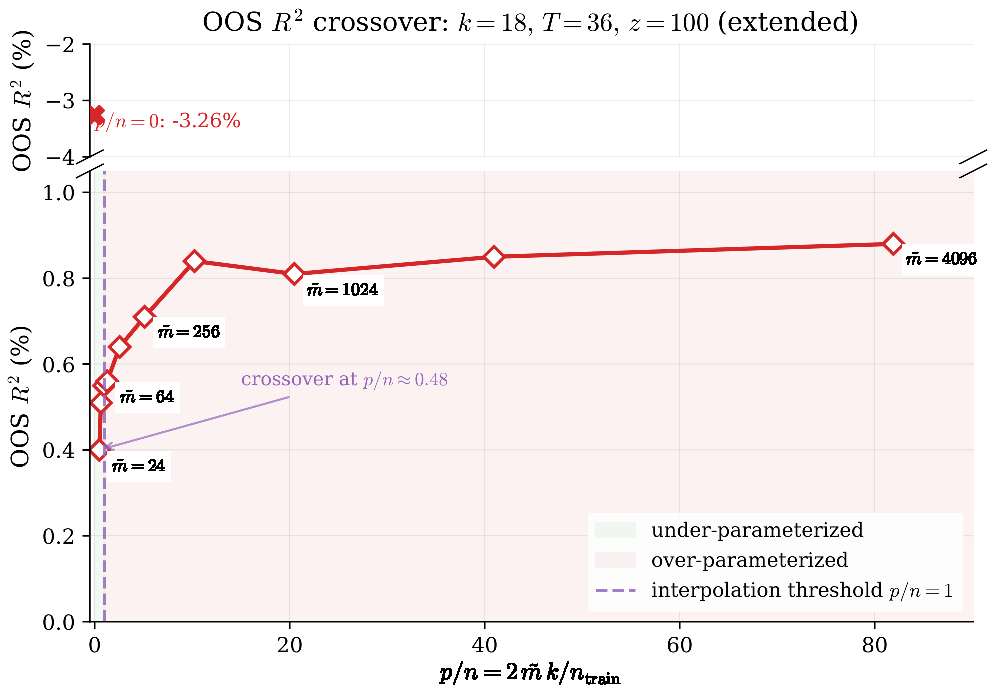
\includegraphics[width=0.78\textwidth]{ext_plotA.pdf}
	\caption{Out-of-sample $R^2$ (in percent) versus the parameter ratio
		$p/n=2\tilde m k/n_{\mathrm{train}}$ for $k=18$, $T=36$, and $z=100$.
		The upper panel shows the linear baseline at $p/n=0$ where
		$R^2_{\mathrm{OOS}}=-3.26\%$; the lower panel shows the RFF
		specifications. The shaded regions distinguish the
		under-parameterized and over-parameterized regimes, and the
		dashed vertical line marks the interpolation threshold $p/n=1$.
		The annotated crossover from negative to positive
		$R^2_{\mathrm{OOS}}$ occurs at $p/n\approx 0.48$ ($\tilde m=24$),
		\emph{before} the interpolation threshold.}
	\label{fig:ext_crossover}
\end{figure}

Figure~\ref{fig:ext_r2compare} extends the crossover view by collecting the
full
$R^2_{\mathrm{OOS}}$ curves across the main factor-count and window-length
specifications in the extended grid.

\begin{figure}[H]
	\centering
	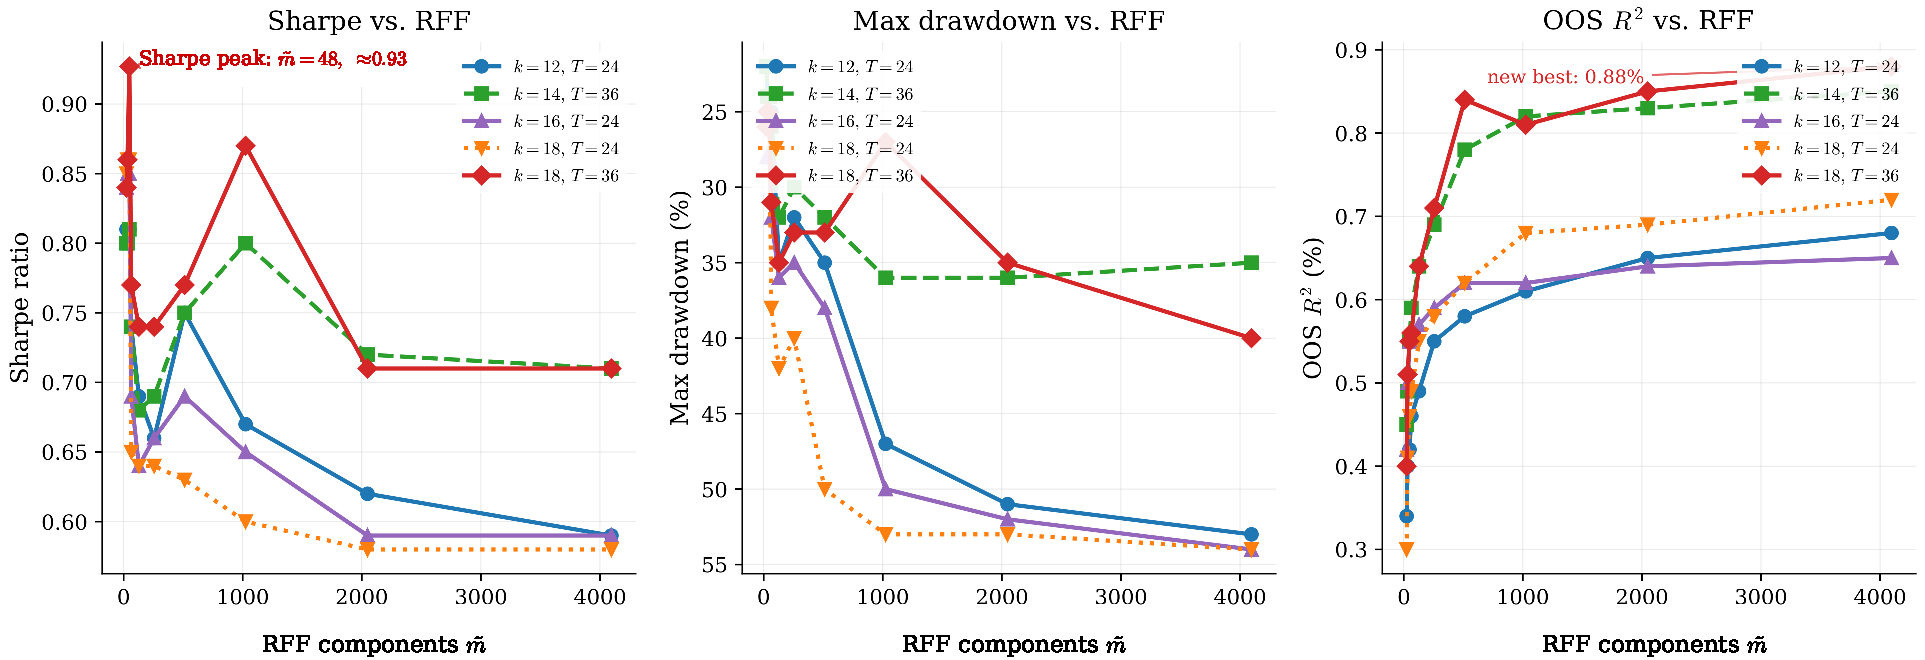
\includegraphics[width=0.78\textwidth,trim=615 0 0 0,clip]{ext_plotI.pdf}
	\caption{Out-of-sample $R^2$ (in percent) across RFF dimensions in the
		extended backtest. The longer-window $k=18,T=36$ specification attains
		the study's new best predictive value of $0.88\%$ at
		$\tilde m=4096$. The figure also shows that the longer-window
		specifications dominate their shorter-window counterparts once the RFF
		dictionary becomes sufficiently rich.}
	\label{fig:ext_r2compare}
\end{figure}

Taken together, Figures~\ref{fig:ext_crossover} and~\ref{fig:ext_r2compare}
show three empirical phases across the two primary specifications,
$k=12,T=24$ and $k=18,T=36$.

First, there is a structural-discovery phase between $\tilde m=0$ and
$\tilde m=24$. The linear baseline has negative out-of-sample $R^2$:
approximately $-4.95\%$ for $k=12,T=24$ and $-3.26\%$ for $k=18,T=36$. By
$\tilde m=24$, both specifications have crossed into positive territory,
reaching approximately $+0.34\%$ and $+0.40\%$, respectively. Since
$\tilde m=24$ corresponds to $p/n=0.48$ in the two primary specifications, the
predictive crossover occurs in the under-parameterized regime.

This early crossover is not just a parameter-count effect. Even at relatively
low complexity, the RFF lift already opens nonlinear interaction channels
among the original characteristics, so the move from the linear baseline to
$\tilde m=24$ can reveal return structure that a purely linear exposure map
cannot express. That helps explain why the sharpest improvement in
$R^2_{\mathrm{OOS}}$ appears before the interpolation threshold is reached.

Second, there is a geometric-refinement phase between $\tilde m=24$ and
$\tilde m=512$. In this range, $R^2_{\mathrm{OOS}}$ continues to improve while
the factor covariance diagnostics become more favorable. This is the range in
which the nonlinear characteristic dictionary becomes rich enough to improve
predictive fit without yet exhausting the stabilizing effect of the training
sample and ridge penalty.

Third, there is a high-complexity improvement phase between $\tilde m=512$ and
$\tilde m=4096$. Predictive performance continues to improve, though with
smaller marginal gains. The best $R^2_{\mathrm{OOS}}$ in the extended study is
$+0.88\%$, attained at $\tilde m=4096$, $k=18$, and $T=36$. The corresponding
$k=12,T=24$ configuration reaches $+0.68\%$ at $\tilde m=4096$.

The multi-configuration comparison also sharpens the ranking across factor
count and training-window length.

The previously reported $k=14,T=36$ specification remains strong throughout
the grid, but the new $k=18,T=36$ curve overtakes it in the richer-feature
region and finishes at the study's best predictive value of $+0.88\%$ at
$\tilde m=4096$.

The shorter-window $k=18,T=24$ configuration also improves monotonically with
$\tilde m$, but it remains below the longer-window counterpart across the
high-complexity tail. The $k=12,T=24$ and $k=16,T=24$ curves rise more
gradually and plateau at materially lower levels, ending near $+0.68\%$ and
$+0.65\%$, respectively. Thus the richer factor structure is most effective
when it is paired with a longer estimation window rather than forced to operate
from the same shorter sample.

This ranking is consistent with the spectral diagnostics developed next.
Moving from $T=24$ to $T=36$ provides roughly 50 percent more training
observations and helps stabilize the larger $k=18$ factor specification. In
particular, the longer-window version maintains a materially higher gap ratio
at large $\tilde m$ than the corresponding $T=24$ specification, which is
consistent with the ridge--curvature mechanism: more training data improve the
estimation of the leading factor directions, while ridge regularization
stabilizes weak trailing directions.

The shorter-window specifications still exhibit useful threshold behavior. In
the $k=12,T=24$ case, the first nonlinear feature expansions already produce a
visible predictive improvement. The main point is not the exact level of
performance, but the fact that the same early nonlinear lift remains visible
even when the training window is shorter, while the longer window is especially
valuable for sustaining larger factor counts and richer feature dictionaries.

Although these values are numerically small, they are economically meaningful
in the context of individual-stock return prediction, where monthly
out-of-sample $R^2$ is often well below one percent. The extended backtest
therefore shows not only an early predictive crossover, but also a clear
high-complexity ranking: longer training windows and sufficiently rich factor
structures allow the nonlinear lift to keep translating into incremental
predictive fit.

\subsubsection{Spectral geometry: effective rank and gap ratio}
\label{sec:extended:spectral}

The extended backtest also clarifies how the factor covariance spectrum changes
with $\tilde m$, $k$, and $T$. Figure~\ref{fig:ext_geom} reports the effective
rank and the gap ratio $\lambda_{\min}/\lambda_{\max}$ of
$\hat\Sigma_f$ across the extended grid.

\begin{figure}[H]
	\centering
	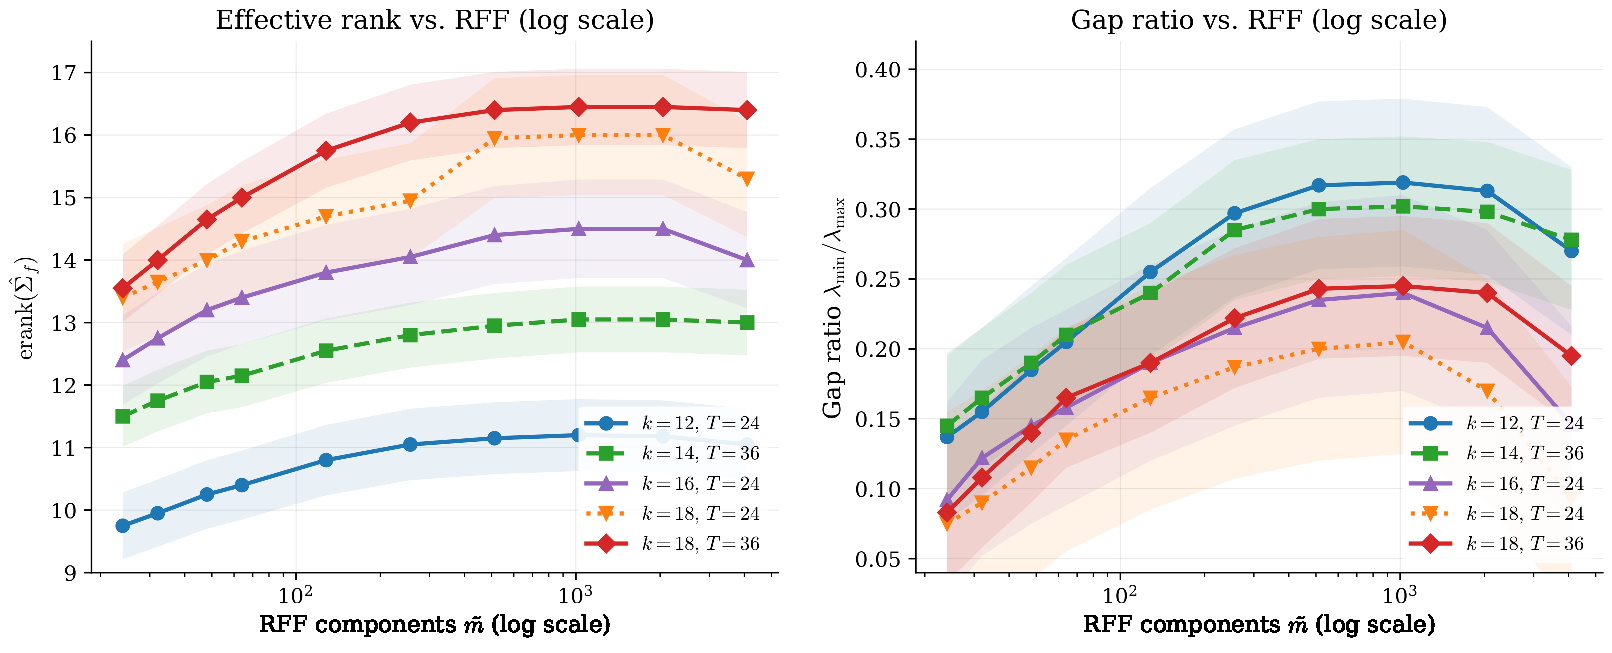
\includegraphics[width=0.92\textwidth]{ext_plotC.pdf}
	\caption{Spectral diagnostics in the extended backtest. Left:
		effective rank $\mathrm{erank}(\hat\Sigma_f)$ versus RFF
		dimension $\tilde m$ on a log scale. Right: gap ratio
		$\lambda_{\min}/\lambda_{\max}$ of the estimated factor
		covariance matrix. Shaded bands indicate $\pm1$ standard
		deviation across RFF seeds. The longer $T=36$ training window
		helps preserve the gap ratio for the larger $k=18$
		specification at high $\tilde m$, whereas the corresponding
		shorter-window specification ($k=18,T=24$) shows greater
		spectral compression.}
	\label{fig:ext_geom}
\end{figure}

The results extend the spectral-gap analysis from
Section~\ref{sec:specgap}. For $k=12,T=24$, the gap ratio rises from about
$0.098$ at low $\tilde m$ to roughly $0.319$ near $\tilde m=1024$, and remains
positive at $\tilde m=4096$. This indicates that the $k=12$ specification remains
spectrally well separated across the RFF range.

The $k=18$ specifications display a stronger dependence on the training
window. For $k=18,T=36$, the gap ratio peaks near $\tilde m=1024$ and remains
approximately $0.195$ at $\tilde m=4096$. By contrast, the corresponding
shorter-window specification has a substantially lower high-$\tilde m$ gap ratio,
around $0.093$. Thus the longer window appears to mitigate the spectral
compression that can arise when a larger fitted factor dimension is combined
with a large nonlinear feature dictionary.

This behavior is consistent with the curvature mechanism in
Theorem~\ref{thm:curv-erank}. Increasing $T$ supplies more observations for
estimating the signal eigenstructure, making it easier to keep the leading
factor directions separated from the empirical noise floor. At the same time,
the continued rise in $R^2_{\mathrm{OOS}}$ through large $\tilde m$ shows that
spectral stability and nonlinear feature expansion can reinforce one another
when the training window is sufficiently long and the ridge penalty is strong.

\subsubsection{Subspace stability across RFF dimensions}
\label{sec:extended:stability}

The next question is whether the larger RFF dictionaries produce stable
Grassmannian motion or merely increase subspace wandering. Figure
\ref{fig:ext_stability} reports three stability diagnostics across $\tilde m$:
the mean geodesic Grassmann distance, the maximum principal angle, and the
projection distance.

\begin{figure}[H]
	\centering
	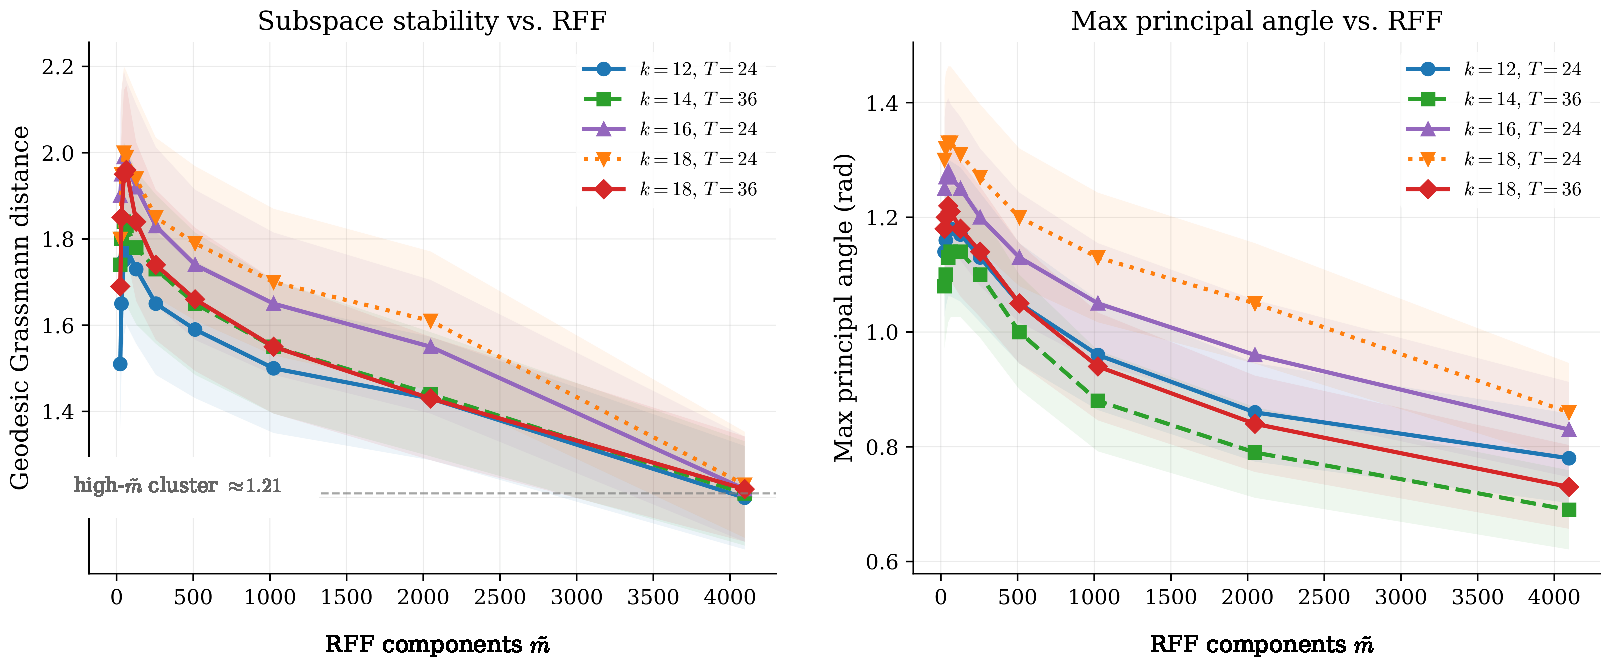
\includegraphics[width=0.92\textwidth]{ext_plotD.pdf}
	\caption{Subspace stability diagnostics in the extended backtest.
		Left: mean geodesic Grassmann distance versus $\tilde m$, with the
		gray dashed line marking the high-$\tilde m$ cluster level
		$\approx 1.21$ that all configurations approach. Right:
		maximum principal angle $\psi_{\max}$ versus $\tilde m$ in radians.
		Shaded bands indicate $\pm1$ standard deviation across RFF
		seeds. Across the configurations studied, the high-$\tilde m$ region
		exhibits a common stability profile rather than uncontrolled
		Grassmannian wandering.}
	\label{fig:ext_stability}
\end{figure}

The first notable pattern is that the geodesic distance approaches a common
high-$\tilde m$ level across the configurations studied. At $\tilde m=4096$, the curves
cluster near $d_{\mathrm{geo}}\approx 1.21$. This should not be interpreted
as a universal constant of the model, but it is a striking empirical regularity
in this extended grid. The high-$\tilde m$ subspace trajectories appear to settle
into a common stability regime rather than diverging across factor counts and
training-window lengths.

For reference, the expected geodesic distance between two independent
Haar-random subspaces of comparable dimension in a 50-dimensional ambient space
is larger, roughly $1.4$--$1.5$ radians. The observed high-$\tilde m$ distances
therefore remain below the scale of independent random rotations, suggesting
partial persistence of the estimated signal subspace rather than directionless
month-to-month wandering.

The maximum principal angle provides a complementary view. After the small-$\tilde m$
region, $\psi_{\max}$ declines as $\tilde m$ increases, indicating that the
largest single subspace rotation becomes smaller in richer RFF dictionaries.
This is consistent with the Goldilocks interpretation developed in
Section~\ref{sec:goldilocks}: useful configurations are not those with maximal
subspace motion, but those in which movement is controlled and concentrated.
The projection-distance diagnostic shows the same broad message. It rises out
of the frozen regime, reaches an intermediate region, and then stabilizes or
declines rather than exploding at large $\tilde m$.

Taken together, the extended backtest sharpens the historical picture in three
ways. First, it makes the interpolation boundary visible:
$R^2_{\mathrm{OOS}}$ crosses zero before $p/n=1$, consistent with
Theorem~\ref{thm:pop-signal-subspace} and with the view that the signal
subspace can become accessible before the nominal interpolation threshold is
reached. Second, it clarifies the role of training-window length. The longer
$T=36$ window materially weakens the high-$\tilde m$ spectral compression seen
at $T=24$, which is consistent with
Theorem~\ref{thm:curv-erank}(ii)--(iii): additional observations stabilize the
signal eigenvalues and preserve curvature along the informative directions.
Third, because the universe is selected on a rolling basis, the same broad
metric patterns appear without relying on the fixed top-50 selection used in
the baseline section. The best extended configuration, $k=18, T=36$, achieves
both the strongest $R^2_{\mathrm{OOS}}$ and the cleanest spectral geometry,
suggesting that a richer factor structure can be beneficial when the sample
size is sufficient to prevent curvature collapse.

At high $\tilde m$, geodesic Grassmann distances converge across the
configurations studied, indicating a common stability regime under strong ridge
regularization rather than uncontrolled wandering. At the same time, the
multi-configuration $R^2_{\mathrm{OOS}}$ comparison shows that the predictive
ranking is not perfectly monotone across intermediate $\tilde m$: some
specifications dip before recovering in the richer-feature region. Since this
pattern is not explained by the current theory and may reflect properties of
the RFF approximation or seed dependence, it should be treated as exploratory
rather than as established structural evidence.

\section{Practitioner Uses}
\label{sec:pract_use}

The diagnostics developed above are intended not only as descriptive tools, but also as practical aids for model design, hyperparameter screening, and ongoing model monitoring. We summarize several practitioner uses.

\smallskip\noindent
\textit{Diagnostic taxonomy.} The empirical results contain several distinct sources of apparent complexity. A specification may be effectively frozen because its fitted subspace barely moves; it may sit near a spectral boundary where weak directions are difficult to estimate; it may be stabilized by ridge regularization; or it may benefit from the larger nonlinear characteristic span generated by the RFF lift. The diagnostics are useful because they separate these mechanisms rather than treating all increases in model complexity as equivalent. In this sense, the taxonomy provides a map from observed performance to its likely geometric source.

\smallskip\noindent 
\textit{Projection distance as a screening device.} The projection-distance diagnostic provides a fast regime classifier that can be computed before running a full out-of-sample backtest. Specifications with $\widetilde d_{\mathrm{proj}}$ near zero can be flagged as frozen and removed from the hyperparameter grid at negligible cost. The diagnostic is not intended to rank all surviving configurations by expected performance. Its purpose is more modest but practically important: to identify specifications that fail to generate meaningful Grassmannian movement in the first place. In large hyperparameter searches, this can substantially reduce the number of models requiring expensive rolling-window evaluation.

\smallskip\noindent
\textit{Ridge sweeps as regularization diagnostics.} A ridge sweep of the training-time geometric diagnostics provides a cheap way to assess whether regularization is stabilizing the fitted subspace or merely suppressing movement. If $d_{\mathrm{proj}}$, $\psi_{\max}$, and $\bar\psi$ remain near zero as the ridge parameter $z$ varies, the configuration is likely frozen. If these diagnostics increase and then stabilize, the plateau identifies a natural range beyond which additional
regularization offers diminishing geometric benefit. Conversely, if the principal-angle spectrum becomes diffuse or unstable as $z$ changes, the configuration may be overly sensitive to regularization. The ridge sweep is not a substitute for out-of-sample evaluation, but it can reduce the number of ridge values that require full backtesting.

\smallskip\noindent
\textit{The spectral-gap cliff as a guide to factor dimension.} The spectral-gap cliff provides a structural guide for selecting the factor dimension $k$. A practitioner can compute the spectral-gap diagnostic over a grid of candidate dimensions and locate the point at which the gap collapses. That point marks an empirical signal boundary: below it, the model may omit relevant directions; above it, the model begins to include weak or unstable directions. Rather than searching blindly over all values of $k$, it is natural to focus attention on a narrow neighborhood of the cliff, including values slightly above it, and to use regularization to stabilize the marginal directions. This turns the choice of $k$ from a purely brute-force tuning problem into a geometry-guided model-selection problem.

\smallskip\noindent
\textit{The Goldilocks zone as a runtime stability monitor.} The Goldilocks zone provides a runtime diagnostic for deployed models. A fitted model can track $d_{\mathrm{proj}}$ across rolling estimation windows. If the distance remains persistently near zero, the model may be frozen and insufficiently adaptive to changing market conditions. If the distance rises well above its historical Goldilocks range, the model may be rotating too aggressively, especially if the principal-angle spectrum becomes diffuse rather than concentrated in a small number of directions. Thus $d_{\mathrm{proj}}$ is useful not only as a design-time diagnostic, but also as an ongoing health indicator for the learned return subspace.

\smallskip\noindent
\textit{Stopping rules for nonlinear feature expansion.} The stabilization of $d_{\mathrm{geo}}$, $\psi_{\max}$, and $d_{\mathrm{proj}}$ provides a practical stopping rule for increasing the number of random Fourier features $P$. Once the Grassmannian stability diagnostics have plateaued, further RFF expansion is unlikely to provide large additional geometric benefit, even if modest predictive gains remain possible. This does not eliminate the need for out-of-sample evaluation, but it offers a computationally cheap way to identify diminishing returns in the nonlinear feature expansion. In practice, the diagnostic can be used to concentrate
backtesting resources on the range of $P$ where the fitted subspace is still changing materially.

\smallskip\noindent
Taken together, these diagnostics suggest a practical workflow. First, use projection distance to eliminate frozen specifications. Second, use spectral gaps to identify a plausible range of factor dimensions. Third, use ridge sweeps to determine whether regularization stabilizes the fitted subspace. Fourth, use the stabilization of Grassmannian distances to decide when further feature expansion has reached diminishing geometric returns. Finally, once a model is deployed, monitor the projection distance and principal-angle spectrum as ongoing indicators of subspace health. The resulting workflow does not replace economic judgment or out-of-sample validation, but it makes the search over complex conditional factor models more interpretable, more efficient, and less reliant on blind hyperparameter tuning.


\section{Conclusion}
\label{sec:conclusion}

The debate over the virtue of complexity in asset pricing is, at its core, a geometric one. Nonlinear exposure maps can greatly expand the parameter space without necessarily expanding the intrinsic dimension of the return signal. The economically relevant object is therefore not the raw parameter vector, but the low-dimensional return-producing subspace selected by the model. Grassmannian geometry provides a natural language for measuring the dimension, stability, curvature, and motion of this subspace.

This paper develops that geometric perspective in the setting of nonlinear IPCA-type models. The central message is that complexity is useful when it expands the admissible signal span while preserving a stable and effectively low-dimensional return subspace. Conversely, complexity is harmful when it primarily introduces weakly identified directions that move diffusely across rolling windows. In this sense, the relevant notion of complexity is not the number of parameters, but the stability and effective dimensionality of the learned return signal.

The synthetic and historical experiments support this interpretation. The spectral-gap and effective-rank diagnostics locate the empirical signal boundary. Projection distance separates frozen configurations from active ones. Principal-angle diagnostics, especially the anisotropy ratio $\rho_\psi=\bar\psi/\psi_{\max}$, distinguish concentrated signal tracking from diffuse subspace instability. Together, these diagnostics provide a coherent geometric explanation for when nonlinear feature expansion improves out-of-sample performance and when it merely creates unstable degrees of freedom.

The diagnostics also have practical value because they are computed from training-window fitted objects and are available before the corresponding out-of-sample returns are observed. They serve three complementary functions:

\smallskip\noindent
1. \textit{Grid narrowing.} The spectral-gap cliff provides a structural guide to the effective signal dimension, while $d_{\mathrm{proj}}$ compared with a Haar baseline identifies frozen configurations. These diagnostics help remove clearly degenerate regions of the hyperparameter grid before expensive out-of-sample evaluation.

\smallskip\noindent
2. \textit{Within-regime ranking.} Among active configurations, drift anisotropy $\rho_\psi$ helps distinguish useful subspace motion from diffuse instability. In the historical experiments, the best-performing configurations have low anisotropy, indicating that subspace drift is concentrated in a small number of principal directions rather than spread evenly across weak directions.

\smallskip\noindent
3. \textit{Deployment monitoring.} The Goldilocks region for $d_{\mathrm{proj}}$ provides a runtime stability diagnostic. Persistently small values indicate a model that may be insufficiently adaptive, while very large values warrant inspection for diffuse or unstable subspace motion. Similarly, stabilization of $d_{\mathrm{geo}}$ as the RFF dimension increases provides a useful stopping criterion for feature expansion.

One of the most distinctive empirical findings is that the strongest Sharpe ratios occur slightly beyond the spectral-gap cliff, at $k=20$--$24$, rather than deep inside the clearly identified regime. In the clean synthetic experiments, peak performance occurs closer to the true signal dimension. The historical result therefore suggests that mild overparameterization, when paired with sufficiently strong ridge regularization, can be productive: the additional directions enrich the admissible representation of the return subspace, while regularization suppresses the instability that would otherwise arise from weak curvature and near-null directions. This interpretation is consistent with the curvature analysis of Theorem~\ref{thm:curv-erank} and provides a geometric rationale for the empirical success of modest overparameterization with strong regularization.

Overall, the paper reframes the virtue of complexity as a question about subspace geometry. Complexity is beneficial when it enlarges the set of available signal subspaces while preserving concentrated, stable, and economically meaningful motion. It becomes detrimental when it produces diffuse, weakly identified, or noise-dominated directions. This distinction is the geometric content of the virtue of complexity.


\appendix
\section{Geometric Preliminaries on the Grassmann Manifold}
\label{sec:grass_geom}

This section collects the geometric facts about the Grassmann manifold used throughout the paper. The material is standard; see, for example, \cite{AMS08,BZA24}. We include it here to make the later population arguments self-contained and to clarify the interpretation of the empirical diagnostics.

\subsection{The Grassmann manifold as a space of subspaces}

For integers $1 \le k < N$, the Grassmann manifold $\gr(k,N)$ is the set of all $k$-dimensional linear subspaces of $\bR^N$. A point $V\in \gr(k,N)$ may be represented by any matrix $U\in\mathrm{Mat}_{N,k}(\bR)$ with orthonormal columns such that
\begin{equation*}
V=\mathrm{span}(U), \qquad U^\top U = I_k.
\end{equation*}
Two such representatives determine the same point of $\gr(k,N)$ if and only if they differ by a right orthogonal transformation:
\begin{equation*}
U \sim UO, \qquad O\in O(k).
\end{equation*}
Thus $\gr(k,N)$ may be identified with the quotient
\begin{equation*}
\gr(k,N) = \mathrm{St}(k,N)/O(k),
\end{equation*}
where $\mathrm{St}(k,N)$ denotes the \emph{Stiefel manifold} of orthonormal $k$-frames in $\bR^N$.

Equivalently, a subspace $V\in \gr(k,N)$ may be represented by its orthogonal projector
\begin{equation*}
P_V = UU^\top,
\end{equation*}
which is independent of the chosen orthonormal basis $U$. The projector representation is often convenient because it embeds $\gr(k,N)$ into the space of symmetric matrices:
\begin{equation*}
\begin{split}
P_V^\top &= P_V,\\
P_V^2 &= P_V,\\
\tr(P_V)&=k.
\end{split}
\end{equation*}

\subsection{Tangent space and local coordinates}

Let $V=\mathrm{span}(U)\in \gr(k,N)$, where $U\in \mathrm{St}(k,N)$. The tangent space $T_V\gr(k,N)$ may be identified with
\begin{equation*}
T_V\gr(k,N)= \big\{\Delta\in\mathrm{Mat}_{N,k}(\bR) : U^\top \Delta = 0\big\}.
\end{equation*}
Thus tangent vectors are precisely those perturbations of $U$ that are orthogonal to the current subspace. This removes the non-identifiable directions corresponding to rotations of the basis inside $V$.

With the canonical Riemannian metric inherited from the Frobenius inner product,
\begin{equation*}
\langle \Delta_1,\Delta_2\rangle = \tr(\Delta_1^\top \Delta_2),
\end{equation*}
the norm of a tangent vector is
\begin{equation*}
\|\Delta\| = \|\Delta\|_F.
\end{equation*}

If $\Delta\in T_V\gr(k,N)$ has compact singular value decomposition
\begin{equation*}
\Delta = A \Psi B^\top,
\end{equation*}
where $A\in\mathrm{Mat}_{N,k}(\bR)$, $B\in O(k)$, and $\Psi=\mathrm{diag}(\psi_1,\dots,\psi_k)$, then the geodesic issuing from $V=\mathrm{span}(U)$ in the direction $\Delta$ is given by
\begin{equation*}
U(t)= U B \cos(t\Psi) B^\top + A \sin(t\Psi) B^\top.
\end{equation*}
In particular, the principal-angle coordinates $\psi_i$ determine both the direction and the length of geodesic motion.

\subsection{Principal angles and standard Grassmann distances}
\label{sec:grass_dist}

Let $V_1$ and $V_2$ be two $k$-dimensional subspaces of $\bR^N$. Choose orthonormal basis matrices
\begin{equation*}
U_1,U_2\in\mathrm{Mat}_{N,k}(\bR)
\end{equation*}
such that
\begin{equation*}
\begin{split}
V_i&=\mathrm{span}(U_i),\\
U_i^\top U_i&=I_k,
\end{split}
\end{equation*}
for $i=1,2$. The standard distances between $V_1$ and $V_2$ can be expressed in terms of their principal angles \cite{BZA24}. These angles
\begin{equation*}
\psi_1,\ldots,\psi_k\in[0,\pi/2]
\end{equation*}
are defined by
\begin{equation}
\label{eq:principal-angles}
\cos\psi_i = \sigma_i(U_1^\top U_2), \qquad i=1,\ldots,k,
\end{equation}
where
\begin{equation*}
\sigma_1\geq \cdots \geq \sigma_k\geq 0
\end{equation*}
are the singular values of $U_1^\top U_2$. Equivalently, if
\begin{equation}
\label{eq:svd}
U_1^\top U_2 = Q_1\,\mathrm{diag}(\sigma_1,\ldots,\sigma_k)\,Q_2^\top
\end{equation}
is the singular value decomposition, then
\begin{equation*}
\psi_i=\arccos(\sigma_i).
\end{equation*}
Three distance measures are commonly used.

\noindent
\textit{Geodesic distance.} Equip $\gr(k,N)$ with its canonical Riemannian metric, induced from the quotient representation
\begin{equation*}
\gr(k,N)=\mathrm{St}(k,N)/O(k).
\end{equation*}
The geodesic distance between $V_1$ and $V_2$ is the length of the shortest geodesic connecting them:
\begin{equation}
\label{eq:grass-dist-intrinsic}
d_{\mathrm{geo}}(V_1,V_2)=\inf_{\gamma}\mathrm{Length}(\gamma),
\end{equation}
where the infimum is over all piecewise smooth curves $\gamma:[0,1]\to\gr(k,N)$ satisfying $\gamma(0)=V_1$ and $\gamma(1)=V_2$. In terms of principal angles,
\begin{equation}
\label{eq:grass-dist-theta}
\begin{split}
d_{\mathrm{geo}}(V_1,V_2)&=\Big(\sum_{i=1}^k \psi_i^2\Big)^{1/2}\\
&=\Big(\sum_{i=1}^k \arccos^2\big(\sigma_i(U_1^\top U_2)\big) \Big)^{1/2}.
\end{split}
\end{equation}

\noindent
\textit{Projection distance.} Let
\begin{equation*}
P_i=U_iU_i^\top
\end{equation*}
denote the orthogonal projector onto $V_i$. The projection distance is
\begin{equation}
\label{eq:proj-dist}
d_{\mathrm{proj}}(V_1,V_2) = \|P_1-P_2\|_F .
\end{equation}
In terms of principal angles,
\begin{equation}
\label{eq:proj-theta}
\|P_1-P_2\|_F^2 = 2\,\sum_{i=1}^k \sin^2\psi_i .
\end{equation}

\noindent
\textit{Chordal distance.} The scaled chordal distance is
\begin{equation}
\label{eq:chordal-dist}
\begin{split}
d_{\mathrm{chord}}(V_1,V_2) &= \|\sin\Psi\|_F\\
&=\Big(\sum_{i=1}^k \sin^2\psi_i\Big)^{1/2},
\end{split}
\end{equation}
where
\begin{equation*}
\Psi=\mathrm{diag}(\psi_1,\ldots,\psi_k).
\end{equation*}
Therefore
\begin{equation}
\label{eq:projection-chordal-relation}
d_{\mathrm{proj}}=\sqrt{2}\,d_{\mathrm{chord}}.
\end{equation}
For nearby subspaces, $\sin\psi_i\approx \psi_i$, and hence
\begin{equation}
\label{eq:local-distance-equivalence}
d_{\mathrm{chord}}\approx d_{\mathrm{geo}}.
\end{equation}

Thus the geodesic, projection, and chordal distances are locally equivalent. In empirical applications, projection and chordal distances are often computationally convenient, while the geodesic distance has the advantage of being intrinsic to the canonical Riemannian geometry of $\gr(k,N)$.

\subsection{Projection functionals and curvature intuition}

Many of the objective functions considered in this paper depend on a subspace $V\in \gr(k,N)$ only through the associated projector $P_V$. A typical example is the projection functional
\begin{equation*}
\cJ(V)=\|(I-P_V)r\|^2
\end{equation*}
or its expected version
\begin{equation*}
\cJ(V)=\mathbb{E}\big(\|(I-P_V)r_t\|^2\big).
\end{equation*}
Since $P_V$ is invariant under changes of basis $U\mapsto UO$, such functionals are intrinsically defined on $\gr(k,N)$.

Their first- and second-order behavior is governed by how $P_V$ changes along geodesics. In particular, flat or nearly flat directions on $\gr(k,N)$ correspond to perturbations of $V$ that induce little change in the projection error. This is the geometric origin of the weak-identification phenomena studied in the paper.

\subsection{Haar-uniform random subspaces}

A natural reference distribution on $\gr(k,N)$ is the Haar-uniform law, obtained by choosing a random orthogonal matrix $Q\in O(N)$ with Haar distribution and taking
\begin{equation*}
V = QV_0
\end{equation*}
for any fixed $V_0\in \gr(k,N)$. Because the Haar law is rotation-invariant, the induced distribution of $V$ does not depend on the choice of $V_0$.

Equivalently, if $U\in \mathrm{St}(k,N)$ is obtained by orthonormalizing an $N\times k$ Gaussian random matrix, then $\mathrm{span}(U)$ is Haar-uniform on $\gr(k,N)$.

This distribution provides a natural benchmark for subspace motion. If the observed distance between two fitted subspaces is much smaller than the typical distance between unrelated Haar-random subspaces, the fitted trajectory is unusually persistent or frozen. If it is comparable to the Haar scale, the trajectory is moving on the scale of random reorientation.

\subsection{Haar-normalized projection distance}
\label{subsec:haar_norm}

Let $V\in \gr(k,N)$ be fixed and let $W$ be Haar-uniform on $\gr(k,N)$. A useful benchmark is the typical projection distance between $V$ and an unrelated random $k$-plane.

Write $P_V$ and $P_W$ for the corresponding orthogonal projectors. Then
\begin{equation*}
\begin{split}
d_{\mathrm{proj}}(V,W)^2&=\|P_V-P_W\|_F^2 \\
&=\tr\bigl((P_V-P_W)^\top(P_V-P_W)\bigr) \\
&=2k - 2\tr(P_VP_W).
\end{split}
\end{equation*}
Since
\begin{equation*}
\mathbb{E}\big(\tr(P_VP_W)\big) = \frac{k^2}{N},
\end{equation*}
it follows that
\begin{equation*}
\mathbb{E}\big(d_{\mathrm{proj}}(V,W)^2\big)=\frac{2k(N-k)}{N}.
\end{equation*}
Accordingly, a natural Haar benchmark scale for projection distance is
\begin{equation*}
b_{N,k}=\sqrt{\frac{2k(N-k)}{N}}.
\end{equation*}
In finite samples, one may also use nearby normalizations such as
\begin{equation*}
\sqrt{\frac{2k(N-k)}{N+1}},
\end{equation*}
which differ only slightly for moderate $N$. The precise normalization is less important than the interpretation: it provides the scale of projection distance expected under random subspace orientation.

We therefore define the \emph{Haar-normalized projection distance} by
\begin{equation*}
\widetilde d_{\mathrm{proj}}(V_1,V_2) = \frac{d_{\mathrm{proj}}(V_1,V_2)}{b_{N,k}}.
\end{equation*}
Interpretation is immediate:
\begin{itemize}
\item[(i)] $\widetilde d_{\mathrm{proj}}\ll 1$: subspace motion is much smaller than random, indicating persistence or freezing;
\item[(ii)] $\widetilde d_{\mathrm{proj}}\approx 1$: motion is on the scale of random reorientation;
\item[(iii)] $\widetilde d_{\mathrm{proj}}>1$: motion is unusually large relative to the Haar baseline.
\end{itemize}

This normalization is useful in the empirical sections because raw Grassmann distances depend mechanically on $k$ and $N$. Haar normalization removes much of this scale effect and permits more meaningful comparisons across configurations.

\subsection{Remarks on empirical use}

The Grassmannian diagnostics used in the paper can be organized into three groups. First, \emph{intrinsic-dimension diagnostics}, such as $\erank(\hat\Sigma_f)$, quantify how many directions are effectively active. Second, \emph{subspace-motion diagnostics}, such as $d_{\mathrm{proj}}$, $d_{\mathrm{geo}}$, and principal-angle summaries, quantify the stability of the fitted return span across rolling windows. Third, \emph{normalized diagnostics}, such as Haar-normalized projection distance, calibrate observed motion against the random-subspace benchmark and thereby distinguish genuinely stable tracking from near-random reorientation.

These geometric observables will be the empirical counterparts of the flat-direction and curvature mechanisms developed in Sections~\ref{sec:pop_setup} and~\ref{sec:curvature}.

\section{Proofs of the population theorems}
\label{sec:proofs}

\subsection{Proof of Theorem \ref{thm:pop-signal-subspace}}

Using \eqref{eq:pop-factor-model} and expanding \eqref{eq:pop-functional}, we obtain
\begin{equation*}
\begin{split}
\cJ(V)
&=\mathbb{E}\big(\|(I-\Pi_V)((\beta_t^0)^\top f_t+\varepsilon_t)\|^2\big)\\
&=\mathbb{E}\big(\|(I-\Pi_V)(\beta_t^0)^\top f_t\|^2\big)+\mathbb{E}\big(\|(I-\Pi_V)\varepsilon_t\|^2\big),
\end{split}
\end{equation*}
where the cross term vanishes by Assumption~\ref{A3}. By Assumption~\ref{A1},
\begin{equation*}
\begin{split}
\mathbb{E}\big(\|(I-\Pi_V)\varepsilon_t\|^2\big)
&=\mathbb{E}\big(\varepsilon_t^\top (I-\Pi_V)\varepsilon_t\big)\\
&=\tr\big((I-\Pi_V)\mathbb{E}(\varepsilon_t\varepsilon_t^\top)\big)\\
&=\sigma^2\tr(I-\Pi_V)\\
&= \sigma^2(N-k).
\end{split}
\end{equation*}
This proves \eqref{eq:pop-decomp}.

The signal-loss term is nonnegative and equals zero if and only if
\begin{equation*}
(I-\Pi_V)(\beta_t^0)^\top=0,
\end{equation*}
which is equivalent to
\begin{equation*}
\mathrm{span}\big((\beta_t^0)^\top\big)\subseteq V.
\end{equation*}
Thus the population minimizers are precisely the subspaces $V$ containing $S$. If $k=k_0$, this condition forces $V=S$, proving uniqueness in the exactly specified case.


\subsection{Proof of Theorem \ref{thm:curv-erank}}

By \eqref{eq:pop-grass-functional}, minimizing $\cJ$ over $\gr(k,N)$ is equivalent to maximizing
\begin{equation*}
F(V)=\tr(\Pi_V\Sigma_r).
\end{equation*}

\smallskip
\noindent
\emph{Step 1: Population maximizers.}
Let $\mu_1\geq\cdots\geq\mu_N$ denote the eigenvalues of $\Sigma_r$. By the Ky Fan maximum principle \cite{B97},
\begin{equation}
\label{eq:ky-fan}
\sup_{V\in\gr(k,N)}\,F(V)=\sum_{i=1}^k \mu_i.
\end{equation}
The maximizers are the $k$-dimensional subspaces spanned by eigenvectors associated with the top $k$ eigenvalues. In our model,
\begin{equation*}
\mu_i=
\begin{cases}
\lambda_i,\qquad\text{ for } i=1,\ldots, k_0,\\
\sigma^2,\qquad\text{ for } i=k_0+1,\ldots, N.
\end{cases}
\end{equation*}
Since the noise eigenvalue has multiplicity $N-k_0$, the maximizer is non-unique whenever $k>k_0$. For $k\geq k_0$, every maximizer contains the signal subspace $S=\mathrm{span}(\beta^\top)$.

\smallskip
\noindent
\emph{Step 2: Second variation on the Grassmannian.} Fix a maximizer $V^\star$ and choose an orthonormal basis $U\in\mathrm{St}(k,N)$ for $V^\star$. Let $U_\perp\in\mathrm{St}(N-k,N)$ be an orthonormal basis of $V^{\star\perp}$, so that the matrix $[U\;U_\perp]$ is orthogonal. A tangent direction at $V^\star$ may be represented by a matrix $K\in\mathrm{Mat}_{N-k,k}(\bR)$. A corresponding geodesic representative is
\begin{equation}
\label{eq:grassmann-geodesic-local}
U(\varepsilon)=\big(U+U_\perp K\varepsilon\big)\big(I_k+K^\top K\varepsilon^2\big)^{-1/2},
\end{equation}
with projector
\begin{equation*}
\Pi(\varepsilon)=U(\varepsilon)U(\varepsilon)^\top.
\end{equation*}
Write the block decomposition of $\Sigma_r$ in the basis $[U\;U_\perp]$:
\begin{equation}
\label{eq:block-sigma-r}
\Sigma_r =
\begin{pmatrix}
A_{11} & A_{12} \\
A_{21} & A_{22}
\end{pmatrix},
\end{equation}
where
\begin{equation*}
\begin{split}
A_{11}&=U^\top\Sigma_r U,\\
A_{22}&=U_\perp^\top\Sigma_r U_\perp,\\
A_{12}&=U^\top\Sigma_r U_\perp.
\end{split}
\end{equation*}
Since $V^\star$ is spanned by eigenvectors of $\Sigma_r$, we have $A_{12}=0$. A standard second-order expansion gives
\begin{equation}
\label{eq:second-var}
F(V(\varepsilon))=F(V^\star)-\varepsilon^2\tr\big(K^\top(A_{11}-A_{22})K\big)+o(\varepsilon^2).
\end{equation}
Therefore the Riemannian Hessian of $\cJ=-F+\tr(\Sigma_r)$ at $V^\star$ is, up to the conventional factor of $2$, the quadratic form
\begin{equation*}
K\mapsto \tr\!\big(K^\top(A_{11}-A_{22})K\big).
\end{equation*}

\smallskip
\noindent
\emph{Step 3: Flat directions.}
When $k>k_0$, the subspace $V^\star$ contains $k-k_0$ directions inside the noise eigenspace. Tangent directions that rotate these selected noise directions into unselected noise directions have the same eigenvalue $\sigma^2$ on both sides of the decomposition. Hence the corresponding entries of $A_{11}-A_{22}$ vanish, and the Hessian of $\cJ$ is zero along those directions. This proves part~(i).

\smallskip
\noindent
\emph{Step 4: Eigenvalue-gap curvature.} Now consider a tangent direction that rotates a signal eigenvector with eigenvalue $\lambda_i$ toward a noise eigenvector with eigenvalue $\sigma^2$. In the eigenbasis, the relevant contribution to $A_{11}-A_{22}$ is precisely the gap $\lambda_i-\sigma^2$. Summing over the principal rotation components gives
\begin{equation*}
\mathrm{Hess}_{V^\star}\cJ[\xi,\xi]\asymp\sum_{i=1}^{k_0}(\lambda_i-\sigma^2)\|\xi_i\|^2,
\end{equation*}
which proves part~(ii).

\smallskip
\noindent
\emph{Step 5: Effective rank.} Let $U$ be an orthonormal basis of $V^\star$ and define
\begin{equation*}
f_t^\star=U^\top r_t.
\end{equation*}
Then
\begin{equation*}
\begin{split}
\Sigma_f^\star&=\mathbb{E}(f_t^\star(f_t^\star)^\top)\\
&=U^\top\Sigma_r U\\
&=A_{11}.
\end{split}
\end{equation*}
Since $V^\star$ contains the $k_0$ signal eigenvectors and $k-k_0$ noise eigenvectors, the spectrum of $\Sigma_f^\star$ is
\begin{equation*}
\{\lambda_1,\ldots,\lambda_{k_0},\underbrace{\sigma^2,\ldots,\sigma^2}_{k-k_0\ \mathrm{times}}\}.
\end{equation*}
The effective-rank conclusion follows directly from the definition of effective rank applied to this spectrum. The normalized spectral weights associated with the added noise directions are small whenever their total contribution $(k-k_0)\sigma^2$ is small relative to the signal trace. This proves part~(iii) and completes the proof.


\section{Features set for the asset pricing application}

{\footnotesize
\setlength{\LTleft}{0pt}
\setlength{\LTright}{0pt}
\begin{longtable}{@{} r p{0.17\textwidth} p{0.71\textwidth} @{}}
  \caption{Dictionary of the 73 firm characteristics used as IPCA instruments in the asset-pricing application.}\label{tab:characteristics}\\
  \toprule
  \# & Characteristic & Definition \\
  \midrule
  \endfirsthead

  \multicolumn{3}{@{}l}{\tablename\ \thetable{} -- continued from previous page}\\
  \toprule
  \# & Characteristic & Definition \\
  \midrule
  \endhead

  \midrule
  \multicolumn{3}{r@{}}{Continued on next page}\\
  \endfoot

  \bottomrule
  \endlastfoot

  1 & \texttt{AM} & Assets-to-market: total assets divided by market equity. \\
  2 & \texttt{AbnormalAccruals} & Abnormal accruals: the residual from an industry accrual model. \\
  3 & \texttt{AnnouncementReturn} & Earnings-announcement return measured around the announcement window. \\
  4 & \texttt{AssetGrowth} & Annual growth rate of total assets. \\
  5 & \texttt{BMdec} & Book-to-market ratio using December market equity. \\
  6 & \texttt{Beta} & CAPM beta estimated from a rolling return regression. \\
  7 & \texttt{BetaFP} & Frazzini--Pedersen beta estimated from overlapping daily stock and market returns. \\
  8 & \texttt{BetaLiquidityPS} & Pastor--Stambaugh liquidity beta. \\
  9 & \texttt{BidAskSpread} & Effective bid--ask spread proxy. \\
  10 & \texttt{BookLeverage} & Book leverage: assets relative to book equity. \\
  11 & \texttt{CF} & Cash-flow-to-price: net income plus depreciation divided by market equity. \\
  12 & \texttt{Cash} & Cash-to-assets ratio. \\
  13 & \texttt{ChEQ} & Growth in book equity. \\
  14 & \texttt{ChInv} & Inventory growth. \\
  15 & \texttt{ChInvIA} & Industry-adjusted change in capital investment. \\
  16 & \texttt{ChNWC} & Change in net working capital. \\
  17 & \texttt{ConvDebt} & Indicator for convertible debt issuance. \\
  18 & \texttt{CoskewACX} & Ang--Chen--Xing style coskewness measure. \\
  19 & \texttt{Coskewness} & Coskewness of stock returns with the market. \\
  20 & \texttt{CredRatDG} & Credit-rating downgrade indicator. \\
  21 & \texttt{DebtIssuance} & Debt issuance measure based on growth in debt financing. \\
  22 & \texttt{DelCOA} & Change in current operating assets. \\
  23 & \texttt{DelLTI} & Change in long-term investment. \\
  24 & \texttt{DivInit} & Dividend-initiation indicator. \\
  25 & \texttt{DivOmit} & Dividend-omission indicator. \\
  26 & \texttt{EBM} & Enterprise component of book-to-market. \\
  27 & \texttt{EquityDuration} & Equity-duration measure. \\
  28 & \texttt{ExchSwitch} & Indicator for an exchange switch during the previous year. \\
  29 & \texttt{FirmAge} & Months since the firm first appears in CRSP. \\
  30 & \texttt{GrSaleToGrOverhead} & Sales growth minus overhead-expense growth. \\
  31 & \texttt{Herf} & Industry concentration measured by a sales-based Herfindahl index. \\
  32 & \texttt{High52} & Price relative to the previous 52-week high. \\
  33 & \texttt{IdioVolAHT} & Idiosyncratic volatility from CAPM residuals. \\
  34 & \texttt{Illiquidity} & Amihud illiquidity measure. \\
  35 & \texttt{IndIPO} & Indicator for firms that recently went public. \\
  36 & \texttt{IndMom} & Industry momentum. \\
  37 & \texttt{IntMom} & Intermediate-horizon momentum, using returns from months $t-12$ to $t-6$. \\
  38 & \texttt{InvestPPEInv} & One-year change in property, plant, and equipment plus inventory, scaled by assets. \\
  39 & \texttt{LRreversal} & Long-run reversal based on returns from months $t-36$ to $t-13$. \\
  40 & \texttt{MRreversal} & Medium-run reversal based on returns from months $t-18$ to $t-13$. \\
  41 & \texttt{MaxRet} & Maximum daily return over the previous month. \\
  42 & \texttt{Mom12m} & Standard 12-month momentum. \\
  43 & \texttt{Mom12mOffSeason} & Momentum excluding the seasonal same-calendar-month component. \\
  44 & \texttt{Mom6m} & Six-month momentum. \\
  45 & \texttt{MomOffSeason} & Off-season return over the previous year. \\
  46 & \texttt{MomSeason} & Same-calendar-month return seasonality over prior years. \\
  47 & \texttt{MomSeasonShort} & Same-calendar-month return in the previous year. \\
  48 & \texttt{NetDebtFinance} & Net debt financing. \\
  49 & \texttt{NetEquityFinance} & Net equity financing. \\
  50 & \texttt{NumEarnIncrease} & Number of consecutive quarterly earnings increases. \\
  51 & \texttt{PctAcc} & Percent operating accruals. \\
  52 & \texttt{PriceDelayRsq} & Price-delay measure based on the incremental explanatory power of lagged market returns. \\
  53 & \texttt{PriceDelaySlope} & Price-delay measure based on the weighted slope of lagged market-return coefficients. \\
  54 & \texttt{PriceDelayTstat} & Price-delay measure based on the weighted \emph{t}-statistics of lagged market-return coefficients. \\
  55 & \texttt{RDIPO} & Indicator for recent IPO firms with zero R\&D spending. \\
  56 & \texttt{RDS} & Real dirty surplus. \\
  57 & \texttt{RealizedVol} & Realized total volatility from daily returns. \\
  58 & \texttt{ResidualMomentum} & Momentum computed from Fama--French three-factor residual returns. \\
  59 & \texttt{ReturnSkew} & Skewness of daily returns over the previous month. \\
  60 & \texttt{ReturnSkew3F} & Skewness of idiosyncratic returns from a Fama--French three-factor model. \\
  61 & \texttt{SP} & Sales-to-price ratio. \\
  62 & \texttt{ShareRepurchase} & Share-repurchase indicator. \\
  63 & \texttt{Spinoff} & Spinoff-event indicator. \\
  64 & \texttt{Tax} & Taxable-income-to-income measure. \\
  65 & \texttt{VolMkt} & Dollar trading volume scaled by market equity. \\
  66 & \texttt{VolSD} & Rolling standard deviation of trading volume. \\
  67 & \texttt{VolumeTrend} & Time trend in trading volume. \\
  68 & \texttt{betaVIX} & Sensitivity of stock returns to changes in the VIX. \\
  69 & \texttt{cfp} & Operating cash-flow-to-price ratio. \\
  70 & \texttt{dNoa} & Change in net operating assets. \\
  71 & \texttt{hire} & Employment growth. \\
  72 & \texttt{Size} & Log market capitalization. \\
  73 & \texttt{STreversal} & Short-term reversal based on the previous month's return. \\
\end{longtable}
}


\medskip\noindent
\textbf{Declaration of generative AI and AI-assisted technologies in the manuscript preparation process}: During the preparation of this work, the authors used ChatGPT (OpenAI) and Claude (Anthropic) for language editing and stylistic refinement of portions of the manuscript. All substantive ideas, models, derivations, and conclusions are solely those of the authors. After using these tools, the authors reviewed and edited the content as needed and takes full responsibility for the
content of the published article.


\begin{thebibliography}{99}
	
\bibitem{AMS08} Absil, P.-A., Mahony, R., and Sepulchre, R.: \emph{Optimization Algorithms on Matrix Manifolds}, Princeton University Press, (2008).

\bibitem{AL26} Afsharhajari, N., and Li, J. Y.-M.: The Virtue of Sparsity in Complexity, arXiv:2604.17166v1 (2026).

\bibitem{BZA24} Bendokat, T., Zimmermann, R., and Absil, P.-A.:  A Grassmann manifold handbook: basic geometry and computational aspects, \emph{Advances in Computational Mathematics}, \textbf{50}, 6 (2024).

\bibitem{B97} Bhatia, R.: \emph{Matrix Analysis}, Springer Verlag (1997).

\bibitem{B23} Boumal, N.: {\em An Introduction to Optimization on Smooth Manifolds}, Cambridge University Press (2023).

\bibitem{GKX20} Gu, S., Kelly, B., and Xiu, D.: Empirical asset pricing via machine learning, {\em Review of Financial Studies}, \textbf{33}, 2223--2273 (2020).

\bibitem{GW08} Goyal, A., and Welch, I.: A comprehensive look at the empirical performance of equity premium prediction, \textit{Review of Financial Studies}, \textbf{21}, 1455 - 1508 (2008).

\bibitem{KM25} Kelly, B., and Malamud, S.: Understanding the Virtue of Complexity, SSRN 5346842 (2025).

\bibitem{KMZ24} Kelly, B., Malamud, S. and Zhou, K.: The Virtue of Complexity in Return Prediction, \textit{The Journal of Finance}, \textbf{79}, 459 - 503 (2024).

\bibitem{KPS19} Kelly, B., Pruitt, S., and Su, Y.: Characteristics are Covariances: A Unified Model of Risk and Return, \emph{Journal of Financial Economics}, \textbf{134}, 501 - 524 (2019).

\bibitem{KPS20} Kelly, B. T., Pruitt, S., and Su, Y.: Instrumented principal component analysis, SSRN 2983919 (2020).

\bibitem{KW21} Koep, N., Weichwald, S., et al.: \texttt{PyManopt}: A Python Toolbox for Optimization on Manifolds using Automatic Differentiation, {\em Journal of Machine Learning Research}, \textbf{22}, 1--5 (2021).

\bibitem{LM26} Lesniewski, A., and Missaoui, O.: Macro-Conditioned Factor Models on the Grassmannian, SSRN 6565898 (2026).

\bibitem{RR07} Rahimi, A., and Recht, B.: Random Features for Large-Scale Kernel Machines, \textit{Advances in neural information processing systems}, \textbf{20} (2007).

\bibitem{RR08} Rahimi, A., and Recht, B.: Weighted sums of random kitchen sinks: Replacing minimization with randomization in learning, \textit{Advances in neural information processing systems}, \textbf{21} (2008).

\bibitem{RV07} Roy, O., and Vetterli, M.: The effective rank: A measure of effective dimensionality, \emph{2007 15th European Signal Processing Conference}, 606 - 610, Poznan, Poland, (2007).

\end{thebibliography}

\end{document}
